\documentclass{article}

\usepackage[main]{neurips_2026}


\usepackage[utf8]{inputenc} % allow utf-8 input
\usepackage[T1]{fontenc}    % use 8-bit T1 fonts
\usepackage{hyperref}       % hyperlinks
\usepackage{url}            % simple URL typesetting
\usepackage{booktabs}       % professional-quality tables
\usepackage{amsfonts}       % blackboard math symbols
\usepackage{nicefrac}       % compact symbols for 1/2, etc.
\usepackage{microtype}      % microtypography

\usepackage{enumitem}
\usepackage{float}


\usepackage{amssymb,amsthm,mathtools,bm}
\usepackage{multirow}
\usepackage{wrapfig}
\usepackage[table]{xcolor}

\theoremstyle{plain}
\newtheorem{theorem}{Theorem}
\newtheorem{proposition}{Proposition}
\newtheorem{lemma}{Lemma}
\newtheorem{corollary}{Corollary}
\theoremstyle{definition}
\newtheorem{definition}{Definition}
\newtheorem{assumption}{Assumption}
\theoremstyle{remark}
\newtheorem{remark}{Remark}

\newcommand{\ip}[2]{\left\langle#1,#2\right\rangle}
\newcommand{\softmax}{\mathrm{softmax}}
\newcommand{\rms}{\mathrm{rms}}

\usepackage{array}
\newcolumntype{L}[1]{>{\raggedright\let\newline \\\arraybackslash\hspace{0pt}}m{#1}}
\newcolumntype{C}[1]{>{\centering\let\newline \\\arraybackslash\hspace{0pt}}m{#1}}
\newcolumntype{R}[1]{>{\raggedleft\let\newline \\\arraybackslash\hspace{0pt}}m{#1}}


\title{Massive Activations as Gradient Regulators in Pre-Norm Transformers}
\author{
    Yihong Chen \\
    Department of Electronic Engineering\\
    Tsinghua University\\
    Beijing, China \\
    \texttt{chenyihong@tsinghua.edu.cn} \\
    \And
    Quanming Yao \\
    Department of Electronic Engineering\\
    Tsinghua University\\
    Beijing, China \\
    \texttt{qyaoaa@tsinghua.edu.cn} \\
}


\begin{document}
\maketitle

\begin{abstract}
Attention sinks and massive activations are recurring and closely related phenomena in Transformer models. Existing studies have largely focused on the forward pass, leaving open whether their connection is a direct structural consequence or is mediated by a training-time mechanism. We study this question from the perspective of backpropagation. Empirically and theoretically, we show that under causal masking, attention sinks can induce pronounced gradient concentration, which we term \emph{gradient sinks}. In pre-norm architectures with RMSNorm, massive activations can be understood as adaptive regulators of this localized gradient pressure during training. This interpretation predicts that attenuating sink-induced gradients should weaken massive activations. We test this prediction with V-scale, a modification that adjusts value-path backpropagated gradients. In pretrained V-scale models, attention sinks are preserved whereas massive activations are suppressed. These results support gradient sink as a key training-time mediator linking attention sinks and massive activations. Our code is available at \href{https://anonymous.4open.science/}{Anonymous GitHub}.
\end{abstract}

\section{Introduction}

% \footnote{+qm+ for title,
	% something like ``\textit{Massive Activations as Learned Gradient Regulators in Transformers}'' can be better.}
Two prominent and frequently co-occurring phenomena in Transformer-based large language models (LLMs) are \emph{attention sinks} (AS), where a small number of tokens attract disproportionate attention mass~\cite{xiao2024streamingllm,gu2025when}, and \emph{massive activations} (MA), where activations become unusually large on a small set of tokens and features~\cite{bondarenko2023quantizable,sun2024massive,an2025systematic}. 
These phenomena are predominantly observed on the first token and are of significant practical importance for long-context inference~\cite{xiao2024streamingllm,su2025kvsink}, fine-tuning~\cite{liu2026sinktrack,liu2025all,fu2026attention,liu2026surgery}, and quantization~\cite{xiao2023smoothquant,bondarenko2023quantizable,lin2024awq}. Their frequent co-occurrence has also attracted mechanistic interest. AS is predominantly explained as a way to implement ``no-ops'' attention heads that contribute little to the current token~\cite{gu2025when,barbero2025why,guo2025activedormant}, driven by the sum-to-one constraint of the Softmax operator. Yet one question remains unresolved:

\begin{center}
\emph{Why should optimization learn such massive token activations at all?}
\end{center}

Existing explanations have largely approached this question from the forward pass. MA is often described as helping to create sink formation~\cite{sun2024massive,su2026unveiling,queipo-de-llano2026attention}. However, in modern pre-norm architectures, both attention and MLP sublayers operate on normalized inputs~\cite{zhang2019rmsnorm,xiong2020layernorm,touvron2023llama}. Locally, the forward computation depends much more strongly on the direction of representation than on its norm. This makes MA appear somewhat unnecessary or even wasteful. Most interventions in the literature modify trained models post hoc by changing MLP outputs or token activations and observe joint changes in AS and MA. While informative, such interventions do not constitute sufficiently clean causal evidence for their relationship, because both magnitude and direction are perturbed at the same time. Recent works that examine training dynamics~\cite{gallegofeliciano2026hiddendynamics,queipo-de-llano2026attention} provide valuable additional perspectives, but still do not directly isolate the backward mechanism linking sink structure to activation growth. Likewise, showing that AS and MA can be decoupled by architectural changes~\cite{sun2026spike} does not by itself explain why they are learned to be coupled in standard architectures.

We argue that the missing piece lies in backpropagation. Under causal masking, a token that becomes an attention sink is read by many later queries. As a result, sink tokens not only accumulate attention mass in the forward pass, but also accumulate backpropagated gradient contributions from many future positions. This creates a pronounced token-wise gradient imbalance at the post-RMSNorm attention input, where the gradient on the first token becomes substantially larger than that on other tokens. We call this phenomenon a \emph{gradient sink} (GS). In pre-norm Transformers with RMSNorm, such localized gradient pressure can be partially offset because RMSNorm attenuates backpropagated gradients approximately in inverse proportion to activation norm. This suggests a different interpretation of massive activations: rather than being merely the direct mechanistic cause of attention sinks, they may emerge as learned gradient regulators that respond to the gradient imbalance induced by attention sinks and maintain stable residual-stream gradient transport. This interpretation further predicts that relieving sink-induced gradient pressure through an alternative attenuation route should reduce reliance on massive activations even while attention sinks remain present.

The rest of the paper develops and tests this claim in three steps. We first establish empirically that gradient sinks are widespread across Transformer models and show theoretically that, under causal masking, sink structure provides a natural route to gradient aggregation. We then examine how this localized pressure is handled in pre-norm Transformers, showing that RMSNorm-mediated gradient attenuation aligns closely with activation scale, consistent with massive activations acting as gradient regulators. Finally, we test the prediction with \emph{V-scale}, a simple value-path modification for Transformer attention. V-scale applies a norm-dependent radial scaling to value states before attention aggregation and leaves the query-key attention weights unchanged, selectively attenuating the dominant value-path gradients. Across model sizes, V-scale largely preserves attention sink behavior while substantially suppressing massive activations, especially in the residual stream and MLP outputs. Moreover, this modification yields practical benefits. V-scale models show better long-context retrieval performance, including under several post-training quantization settings.

Our contributions are thus threefold. First, we shift the explanation of attention sinks and massive activations from a purely forward-pass story to a backward-pass one by introducing \emph{gradient sinks} as the missing training-time mechanism. Second, we show that in pre-norm RMSNorm Transformers, massive activations can be interpreted as learned regulators of localized gradient pressure. Third, we propose \emph{V-scale}, a simple value-path intervention that turns this mechanism into a causal test and a practical lever for improving long-context retrieval.

% 后续全文结构，每一节专注于一件事情
% 我们到底测什么？
% 为什么 AS 会导致 GS？
% 为什么 GS 会诱导 MA？
% 如果只减轻 gradient pressure，能否在保留 AS 的同时压低 MA？

\section{Preliminaries}
\label{sec:prelim}

Here,
we formalize the Transformer architecture, along with forward and backward observables. These definitions lay the groundwork for studying gradient concentration in subsequent sections.

\paragraph{Pre-norm Transformers}
We study decoder-only Llama-like Transformers with pre-norm residual blocks, RMSNorm, RoPE positional encoding, and SwiGLU MLPs~\cite{touvron2023llama,zhang2019rmsnorm,su2021rope,shazeer2020gluvariants}.
Let $H^\ell = (h_0^\ell,\dots,h_{T-1}^\ell)^\top \in \mathbb{R}^{T\times d_{\mathrm{model}}}$ denote the hidden states inputting to layer $\ell$.
A pre-norm block updates the sequence as
\[\begin{aligned}
    \widetilde H^\ell &= \mathrm{RMSNorm}(H^\ell), &
    R^{\mathrm{attn},\ell} &= \mathrm{Attention}(\widetilde H^\ell), &
    H^{\ell+\frac12} &= H^\ell + R^{\mathrm{attn},\ell}, \\
    \widetilde H^{\ell+\frac12} &= \mathrm{RMSNorm}(H^{\ell+\frac12}), &
    R^{\mathrm{mlp},\ell} &= \mathrm{MLP}(\widetilde H^{\ell+\frac12}), &
    H^{\ell+1} &= H^{\ell+\frac12} + R^{\mathrm{mlp},\ell}.
\end{aligned}\]
The Attention block can be either multi-head attention (MHA)~\cite{vaswani2017attention} or a variant such as grouped-query attention (GQA)~\cite{ainslie2023gqa}. For simplicity, we fix one layer $\ell$ and one attention head $h$, and suppress the layer/head superscripts unless needed. With RoPE, the query, key, and value states at token position $t$ are $q_t = R_t W_Q \widetilde h_t$, $k_t = R_t W_K \widetilde h_t$, and $v_t = W_V \widetilde h_t$, where $R_t\in\mathbb{R}^{d_{\mathrm{head}}\times d_{\mathrm{head}}}$ is the RoPE rotation matrix. Then the causal attention logits and weights are computed by $z_{tj}=\frac{\langle q_t,k_j\rangle}{\sqrt d}+m_{tj}$ and $a_{tj}=\mathrm{softmax}(z_{t,:})_j$, where $m_{tj}=0$ for $j\le t$, and $-\infty$ otherwise.
Finally we have the value aggregation $y_t = \sum\nolimits_{j\le t} a_{tj} v_j$ and head output $o_t = W_O y_t$.

\paragraph{Forward metrics for attention sinks and activations}
For a candidate sink position $s$ (typically the first token, i.e., $s=0$), we follow~\cite{gu2025when,queipo-de-llano2026attention} and use thresholded criteria to count sink-like behavior:
\begin{equation}\label{eq:sink_rate}
    \text{Sink}_s^{\epsilon,\ell} = \frac{1}{H} \sum\nolimits_{h=1}^H \mathbb{I}(\alpha_s^{\ell,h} > \epsilon),
    \quad
    \alpha_s^{\ell,h}=\frac{1}{T_\epsilon}\sum\nolimits_{t=s}^{s+T_\epsilon-1} a_{ts}^{\ell,h},
\end{equation}
where $H$ is the number of attention heads in each layer. Following prior work~\cite{gu2025when} we set the threshold $\epsilon=0.3$ and $T_\epsilon=64$. In this paper, for theory and training dynamics measurements, we also introduce the following simpler column-sum statistics of the attention matrix:
\begin{equation}\label{eq:sink_mass}
\!\!
\overline M_s^{\ell,h} 
\! = \! \frac{M_s^{\ell,h}}{T-s+1} 
\! = \! \frac{1}{T-s+1} \sum\nolimits_{t=s}^{T} a_{ts}^{\ell,h},
\quad
\overline S_s^{\ell,h} 
\! = \! \frac{S_s^{\ell,h}}{T-s+1}
\! = \! \frac{1}{T-s+1}\sum\nolimits_{t=s}^{T} (a_{ts}^{\ell,h})^2.
\end{equation}
The quantity $\overline M_s$ is the average attention mass routed through token $s$ by all causally allowed future queries and $\overline S_s$ is a second-moment version. In experiments, we focus on the first token ($s=0$) and further summarize \eqref{eq:sink_mass} across heads and layers.

For activations, many prior studies identify MA as \emph{single} activation magnitudes that are large where both token and feature axes are considered~\cite{bondarenko2023quantizable,sun2024massive}. 
In this work, we focus on \emph{token-wise} behaviors, so we identify MA as large token-wise activation norms at an explicitly chosen computational site~\cite{guo2025activedormant}, including the input of Transformer layers $\|h_{t,\mathrm{in}}^\ell\|=\|h_t^\ell\|_2$, the output of Transformer layers $\|h_{t,\mathrm{out}}^\ell\|=\|h_t^{\ell+1}\|_2$, and the hidden states after Attention $\|h_{t,\mathrm{half}}^\ell\|=\|h_t^{\ell+{1}/{2}}\|_2$.
We also measure the output of the MLP and the value state.

\paragraph{Backward observables}
We introduce token-wise gradient observables and local gradient-reshaping ratios that expose where gradient pressure is created and how it is subsequently reshaped inside pre-norm residual branches.

Let $\mathcal{L}$ denote the training loss and $\widetilde h_t^{\ell}$ denote the token representation after RMSNorm and before the QKV projections. To quantify gradient behavior at this site, we compare the candidate sink token against a set of early non-sink positions: % TODO 定义一下T_e
\begin{equation}\label{eq:gs_def}
R_{GS}^{\ell}(s) :=
\frac{\|\nabla_{\widetilde h_s^{\ell}} \mathcal{L}\|_2}{\frac{1}{T_e} \sum_{t\le T_e, t\ne s} \|\nabla_{\widetilde h_t^{\ell}} \mathcal{L}\|_2}.
\end{equation}
A model exhibits a gradient sink at position $s$ if $R_{GS}^{\ell}(s)\gg 1$ across a substantial fraction of layers. % 我们为什么不定义一个固定的阈值？因为具体的数值可能与多种因素相关，但是>>1足以体现token间的不均衡性，刻画了最基本的Gradient Sink现象。
Next, 
recalling that $h_t^{\ell+{1}/{2}} = h_t^\ell + r_t^{\mathrm{attn},\ell}$ for Attention blocks, we have $\nabla_{r_t^{\mathrm{attn},\ell}}\mathcal{L} = \nabla_{h_t^{\ell+{1}/{2}}}\mathcal{L}$. Moreover, the difference $\nabla_{h_t^\ell}\mathcal{L} - \nabla_{h_t^{\ell+{1}/{2}}}\mathcal{L}$ isolates the additional gradient contribution propagated through the attention branch, excluding the identity skip path.
We then define three ratios by
\begin{equation}\label{eq:ratios_attn}
\begin{aligned}
    \mathrm{Bloat}_t^{\mathrm{attn},\ell}
    &:= \|\nabla_{\widetilde h_t^\ell}\mathcal{L}\|_2 \,/\, \|\nabla_{r_t^{\mathrm{attn},\ell}}\mathcal{L}\|_2, \\
    \mathrm{Compress}_t^{\mathrm{attn},\ell}
    &:= \|\nabla_{h_t^\ell}\mathcal{L} - \nabla_{h_t^{\ell+{1}/{2}}}\mathcal{L}\|_2 \,/\, \|\nabla_{\widetilde h_t^\ell}\mathcal{L}\|_2, \\
    \mathrm{Change}_t^{\mathrm{attn},\ell}
    &:= \|\nabla_{h_t^\ell}\mathcal{L}\|_2 \,/\, \|\nabla_{h_t^{\ell+{1}/{2}}}\mathcal{L}\|_2
\end{aligned}
\end{equation}
Analogously, we define ratios $\mathrm{Bloat}_t^{\mathrm{mlp},\ell}$, $\mathrm{Compress}_t^{\mathrm{mlp},\ell}$, and $\mathrm{Change}_t^{\mathrm{mlp},\ell}$ in the same way for MLP branch.
% The terminology is chosen to match the observation we later show in Section~\ref{sec:pressure_reshape}.

With above definitions, 
we are ready to examine the training dynamics induced by attention structure. 
Section~\ref{sec:as_to_gs} shows that attention sinks lead to concentrated gradients, forming gradient sinks.
In Section~\ref{sec:pressure_reshape}, 
we analyze how such localized gradient pressure is reshaped by the network and associated with massive activations. 
Finally, Section~\ref{sec:vscale}
validates this mechanism through targeted intervention on the gradient flow.

\section{From attention sink to gradient sink}\label{sec:as_to_gs}

We show both empirically and theoretically that AS induce gradient concentration, 
forming gradient sinks. 
Thus,
we connect forward attention patterns and backward training signals.

\subsection{Empirical observations}

We train \texttt{LlamaForCausalLM} models from scratch and analyze checkpoints throughout training. The models are pretrained on C4 dataset~\cite{raffel2020exploring} using AdamW optimizer.
We consider two model sizes, approximately 0.1B and 0.3B parameters. 
Detailed model and training configurations are listed in Appendix~\ref{app:config}.
We save checkpoints every 1000 steps during training. 
At each checkpoint, we run one forward-backward pass using the same causal language modeling objective as in training and collect token-wise statistics.
Unless otherwise stated, these statistics are averaged over the full evaluation batches, and the AS metrics are additionally averaged over heads.

\begin{figure}[tb]
    \centering
    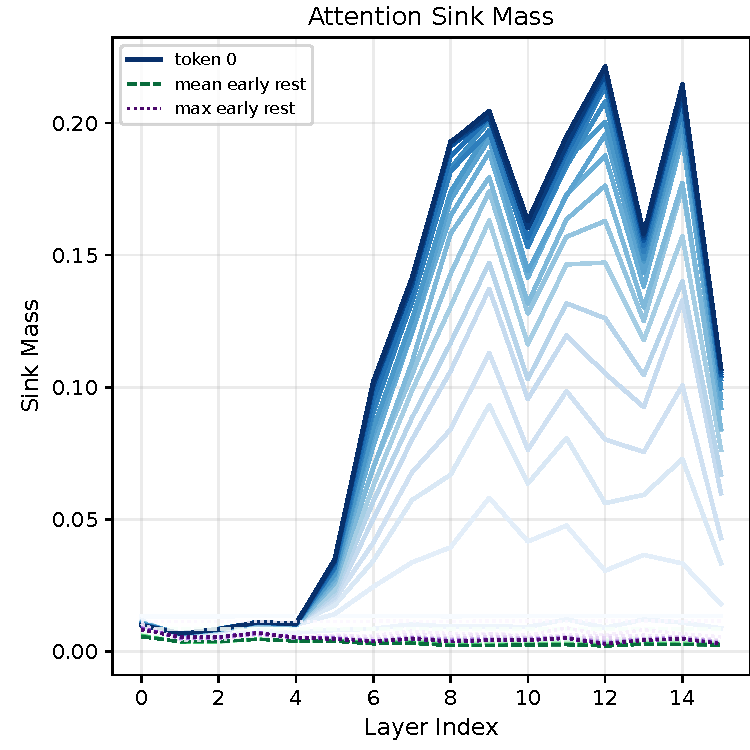
\includegraphics[width=0.23\textwidth]{pics/01B_baseline/AS_mass_compare.pdf}
    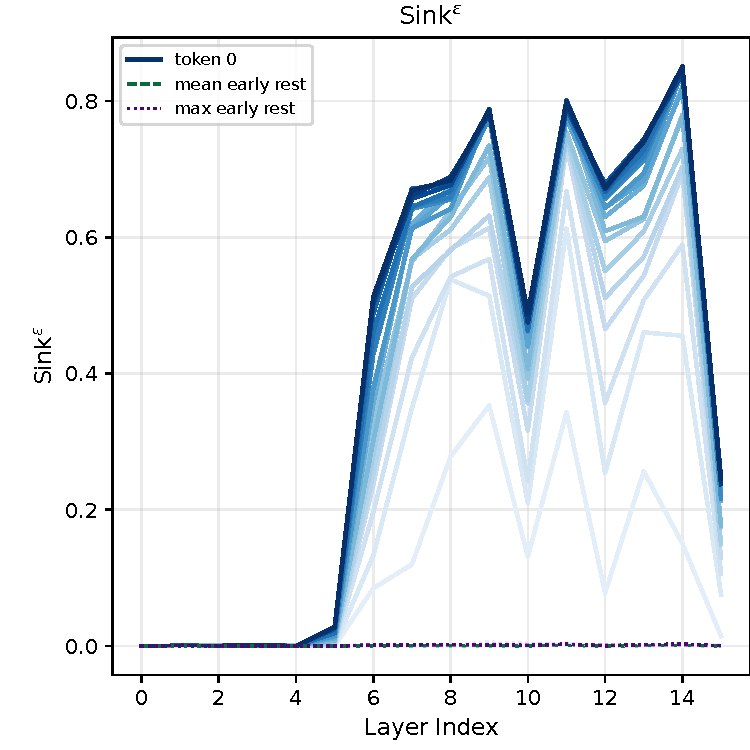
\includegraphics[width=0.23\textwidth]{pics/01B_baseline/AS_eps_compare.pdf}
    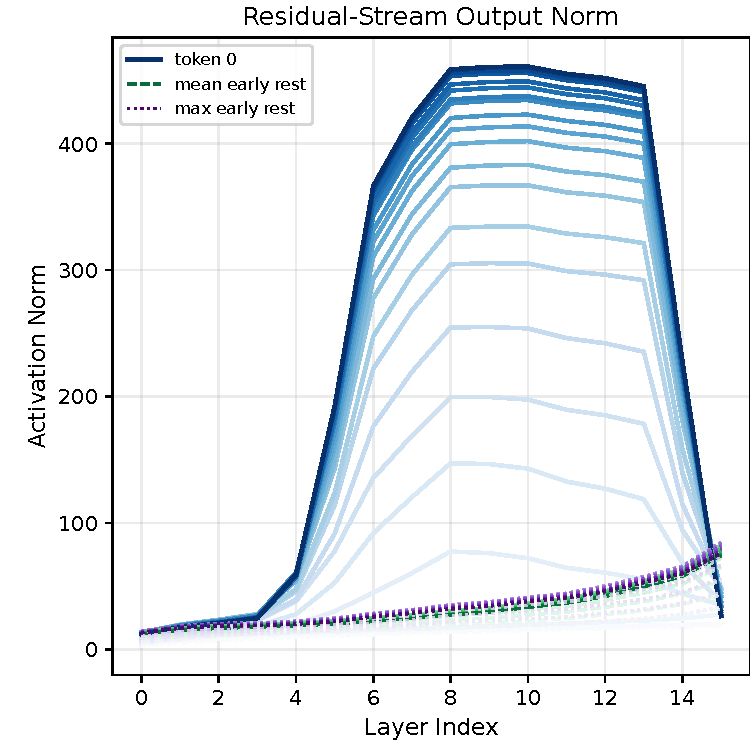
\includegraphics[width=0.23\textwidth]{pics/01B_baseline/MA_x_out_compare.pdf}
    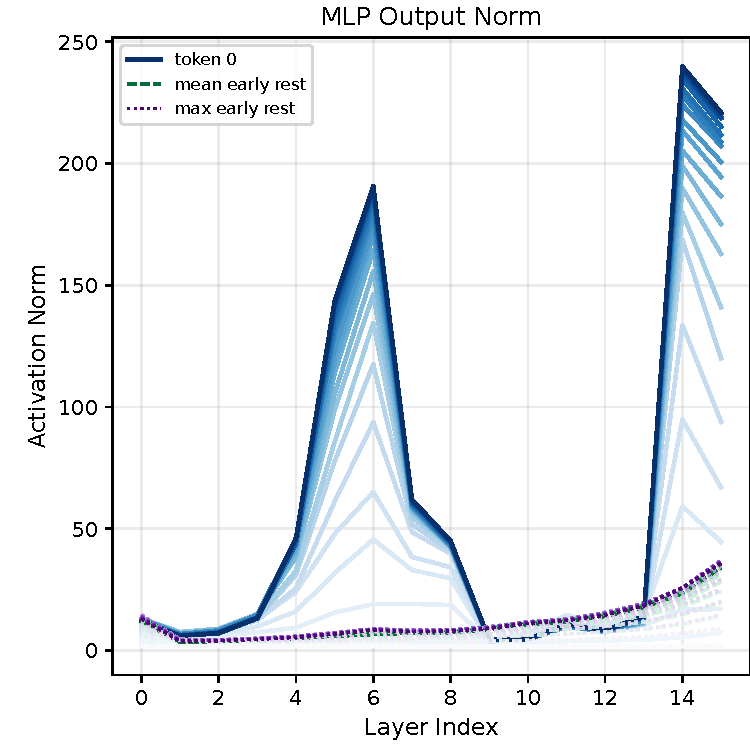
\includegraphics[width=0.23\textwidth]{pics/01B_baseline/MA_mlp_out_compare.pdf}
    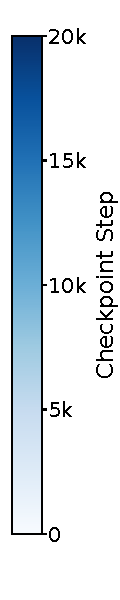
\includegraphics[width=0.046\textwidth]{pics/01B_baseline/extreme_steps.pdf}
    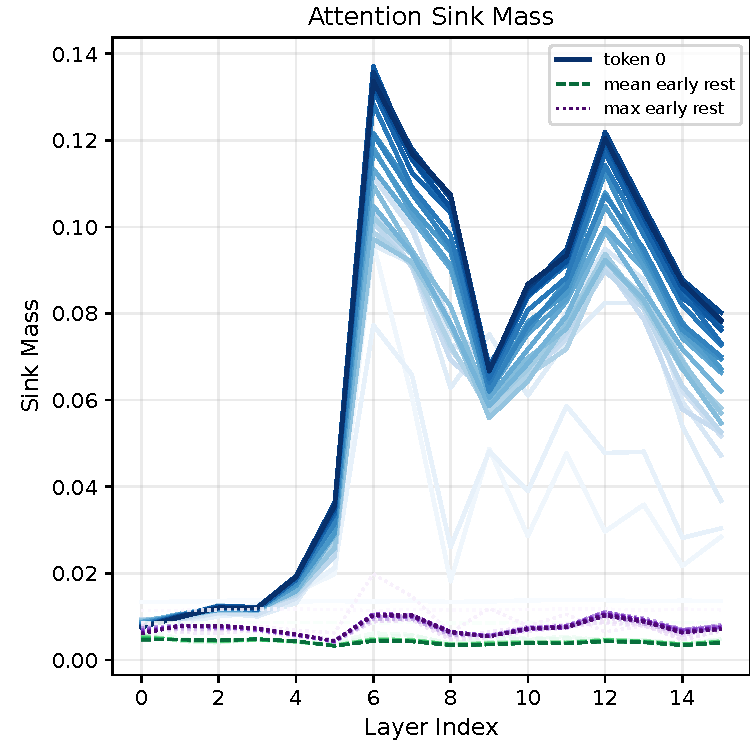
\includegraphics[width=0.23\textwidth]{pics/03B_baseline/AS_mass_compare.pdf}
    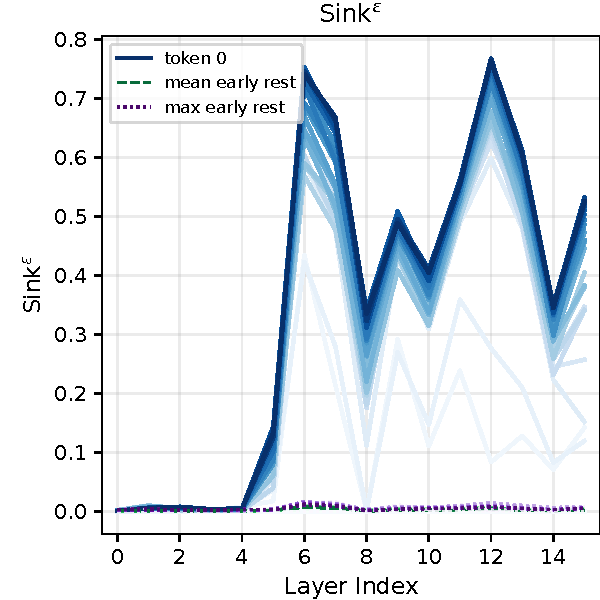
\includegraphics[width=0.23\textwidth]{pics/03B_baseline/AS_eps_compare.pdf}
    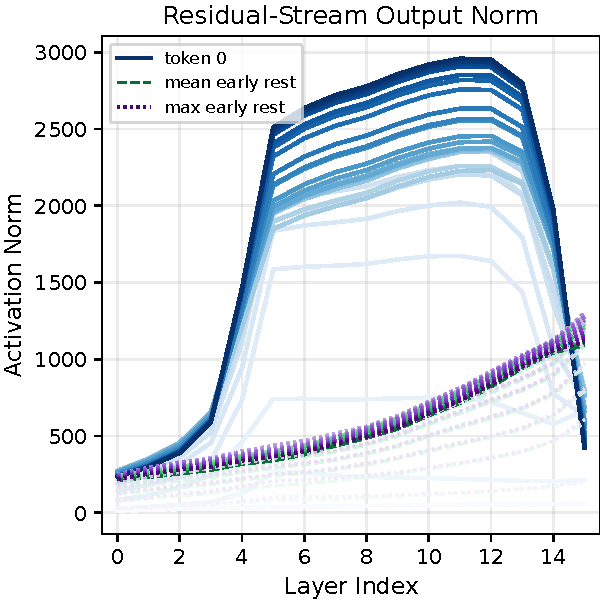
\includegraphics[width=0.23\textwidth]{pics/03B_baseline/MA_x_out_compare.pdf}
    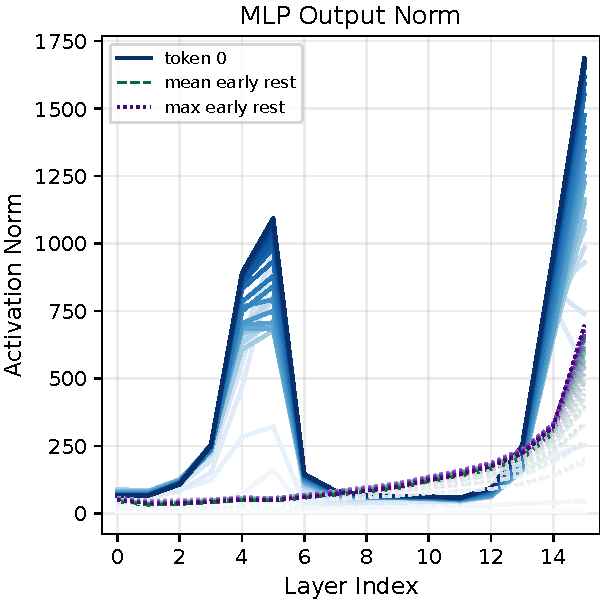
\includegraphics[width=0.23\textwidth]{pics/03B_baseline/MA_mlp_out_compare.pdf}
    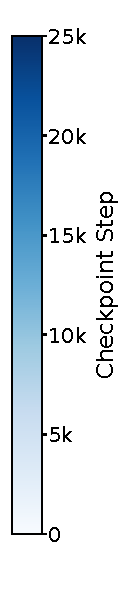
\includegraphics[width=0.046\textwidth]{pics/03B_baseline/extreme_steps.pdf}
    \caption{
    Forward phenomena in baseline models.
    Top row: 0.1B model; bottom row: 0.3B model.
    From left to right: attention sink mass, thresholded sink rate, residual-stream output norm, and MLP output norm.
    We compare the first token (token 0) with the mean and maximum over the rest early tokens (positions 1--15).
    The results confirm the co-occurrence of AS and MA.
    }\label{fig:baseline_forward_main}
\end{figure}

Figure~\ref{fig:baseline_forward_main} summarizes the forward patterns. 
In both model sizes, the sink token is sharply distinguished from the other early tokens on both Sink Mass $\overline M_s^\ell$ 
in \eqref{eq:sink_mass} and $\mathrm{Sink}_s^{\epsilon,\ell}$ in \eqref{eq:sink_rate}. 
On the other hand, the residual outputs at the first token are broadly elevated across layers, and the strongest amplification is concentrated in a small number of MLP blocks. 
These results confirm that AS and MA already co-occur clearly in small pre-norm Transformers.

\begin{figure}[tb]
    \centering
    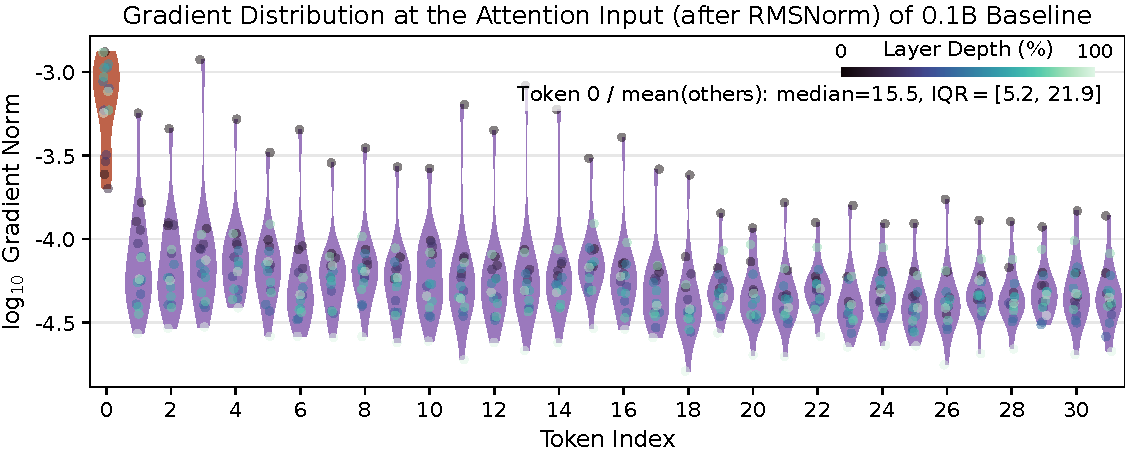
\includegraphics[width=0.48\textwidth]{pics/01B_baseline/violin.pdf}
    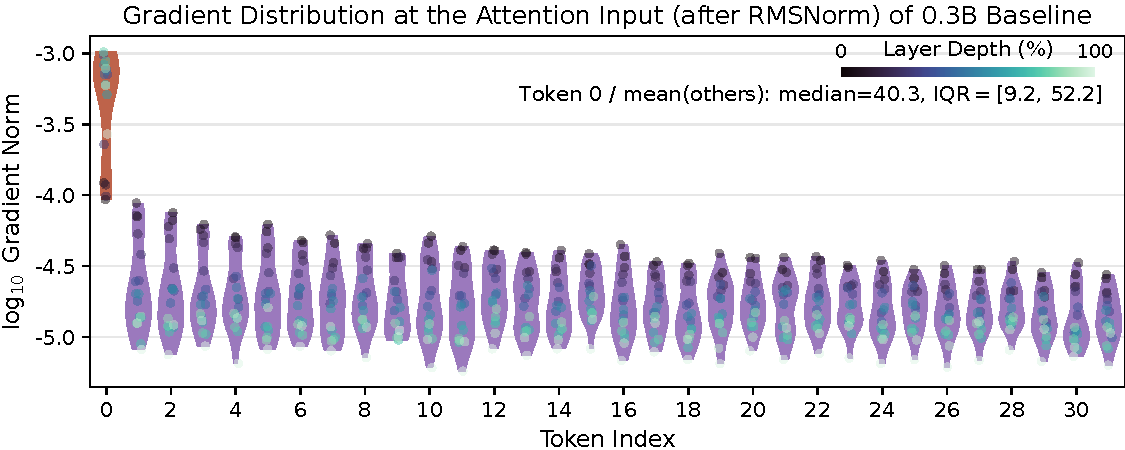
\includegraphics[width=0.48\textwidth]{pics/03B_baseline/violin.pdf}
    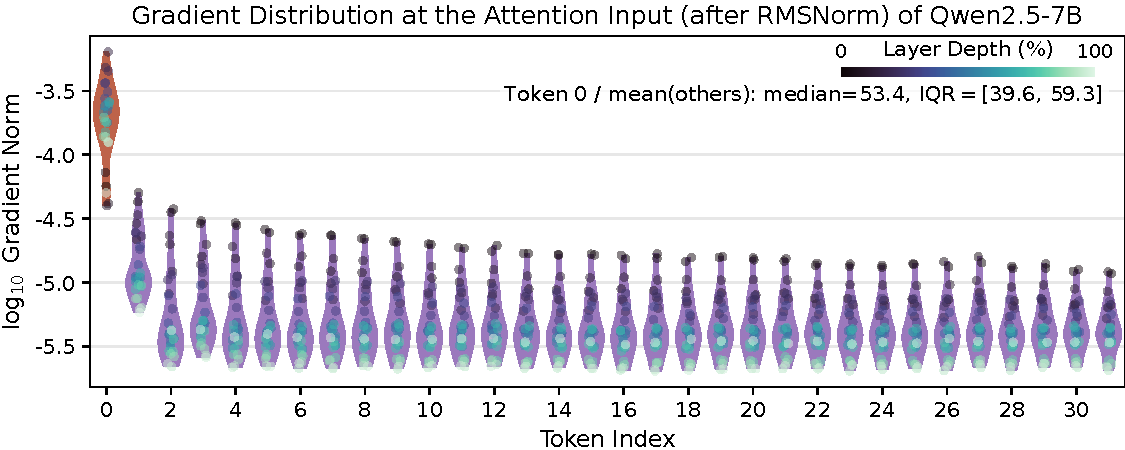
\includegraphics[width=0.48\textwidth]{pics/Qwen2__5_7B/violin.pdf}
    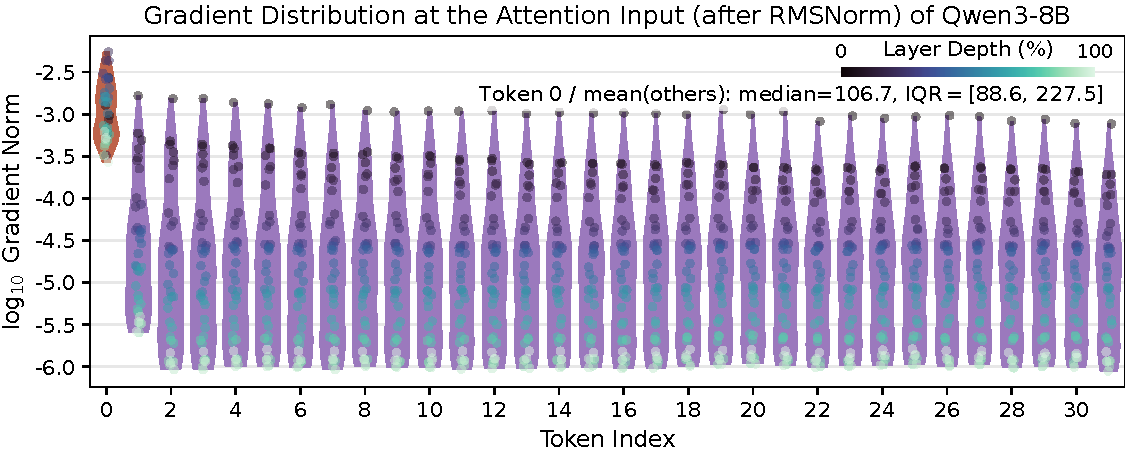
\includegraphics[width=0.48\textwidth]{pics/Qwen3_8B/violin.pdf}
    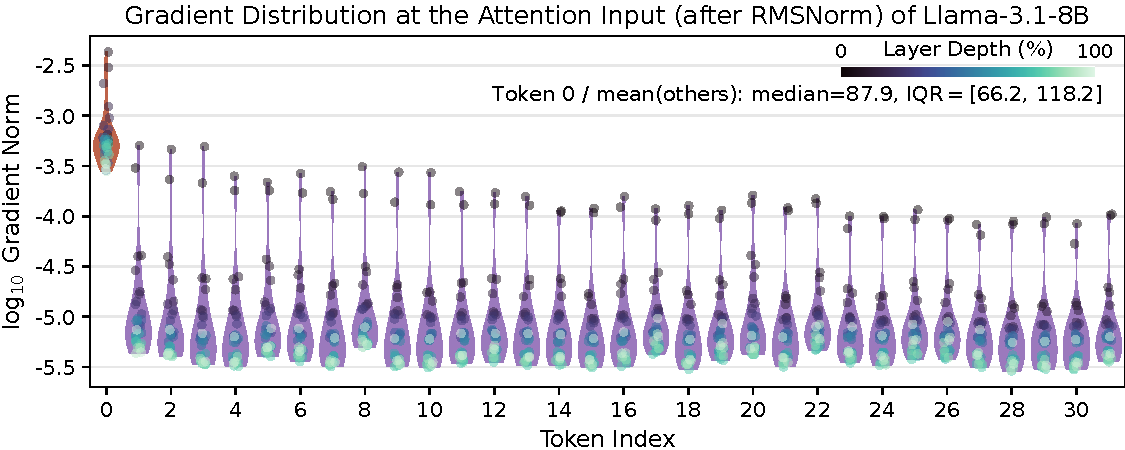
\includegraphics[width=0.48\textwidth]{pics/Llama_3__1_8B/violin.pdf}
    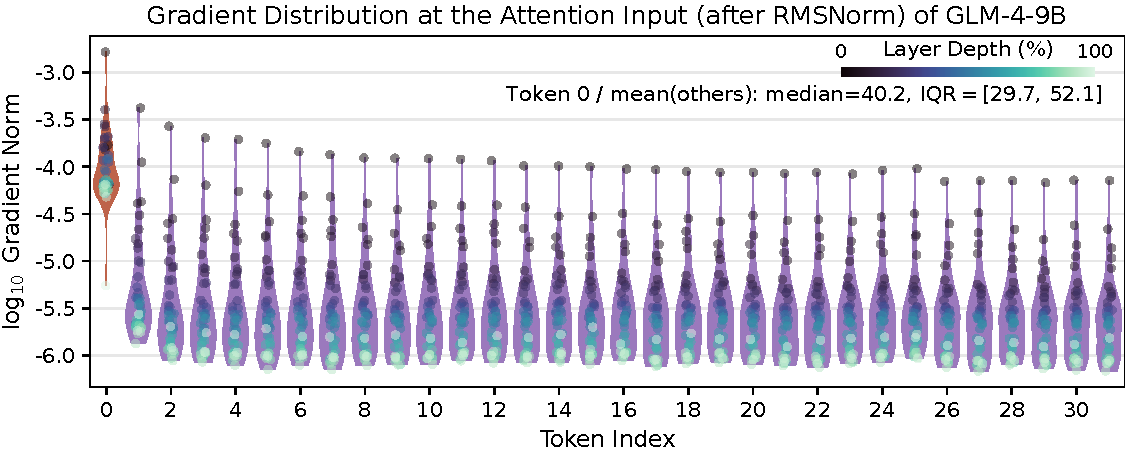
\includegraphics[width=0.48\textwidth]{pics/GLM_4_9B/violin.pdf}
    \caption{Gradient sink phenomenon in pretrained models. Each panel plots the token-wise distribution of $\log_{10}\|\nabla_{\widetilde h_t^{\ell}}\mathcal L\|_2$ at the post-RMSNorm attention input. Token 0 is highlighted while other early tokens share a common color. The median and IQR of $R_{GS}^{\ell}$ are also reported. Models include 0.1B and 0.3B baselines together with Qwen2.5--7B, Qwen3--8B, Llama-3.1--8B, and GLM-4--9B. These show that gradient sinks are a common phenomenon in pretrained models, where the sink token exhibiting substantially larger gradients than other early tokens.
    }\label{fig:gs-definition}
\end{figure}

We now turn to the backward pass and collect the gradients arriving at the post-RMSNorm attention input. We first aggregate gradients over the full batch exactly as in one optimization step, and then take the $l_2$ norm for each token. This makes the resulting token-wise gradients directly comparable to the effective training signal used by the optimizer.
Figure~\ref{fig:gs-definition} shows that the sink token exhibits substantially larger gradients than other early tokens. This significant gradient imbalance is observed in both baseline models and larger pretrained models, suggesting that gradient sink is a common feature of Transformer training dynamics. 

\begin{remark}
While the gradients collected from large pretrained models are computed post hoc under conditions different from their official training, the robust presence of gradient sinks across models and scales suggests it is an intrinsic structural property rather than a sensitive result of specific hyperparameter schedules. 
\end{remark}

\begin{figure}[tb]
    \centering
    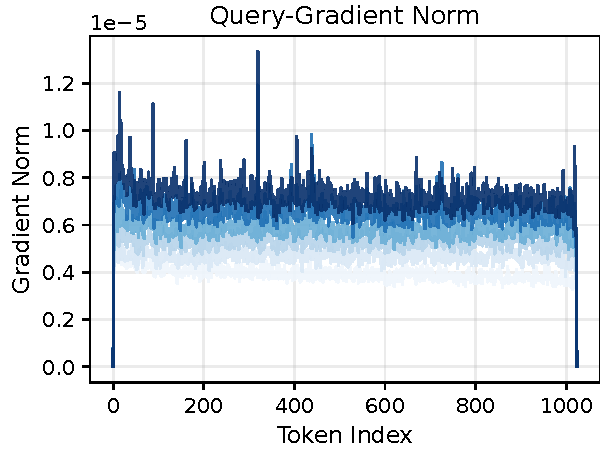
\includegraphics[width=0.3\textwidth]{pics/01B_baseline/LINE_Dq_over_tokens.pdf}
    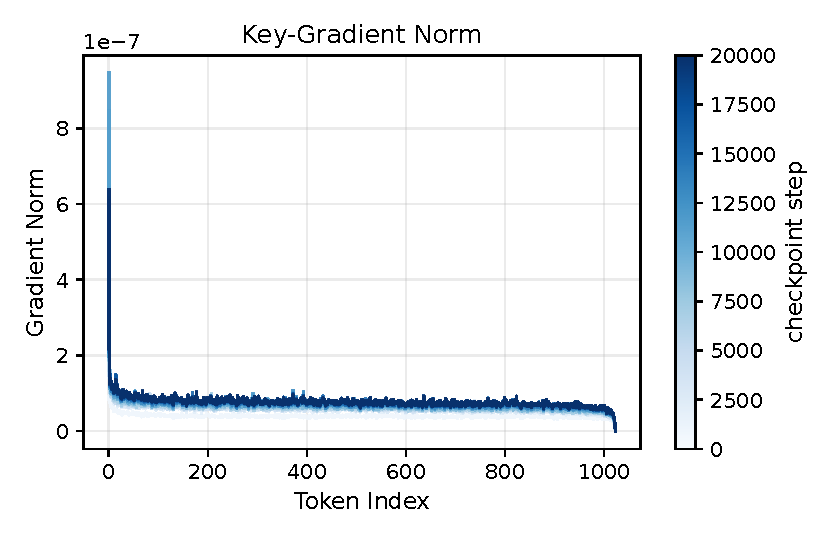
\includegraphics[width=0.3\textwidth]{pics/01B_baseline/LINE_Dk_over_tokens.pdf}
    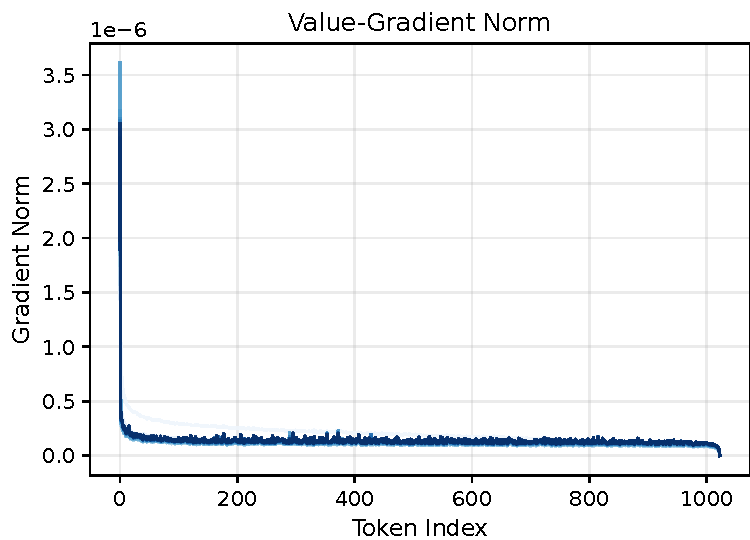
\includegraphics[width=0.3\textwidth]{pics/01B_baseline/LINE_Dv_over_tokens.pdf}
    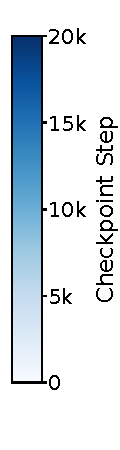
\includegraphics[width=0.06\textwidth]{pics/01B_baseline/line_steps.pdf}
    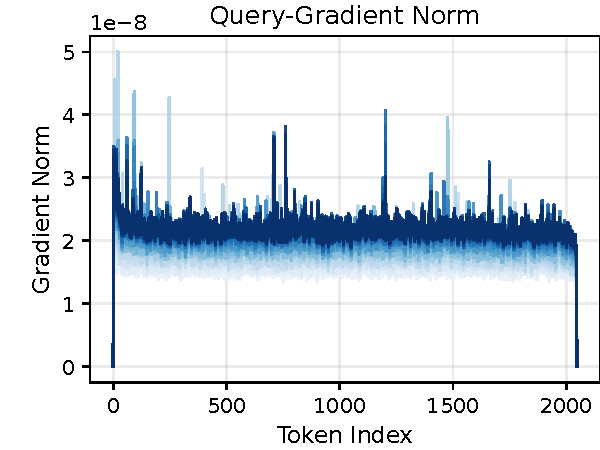
\includegraphics[width=0.3\textwidth]{pics/03B_baseline/LINE_Dq_over_tokens.pdf}
    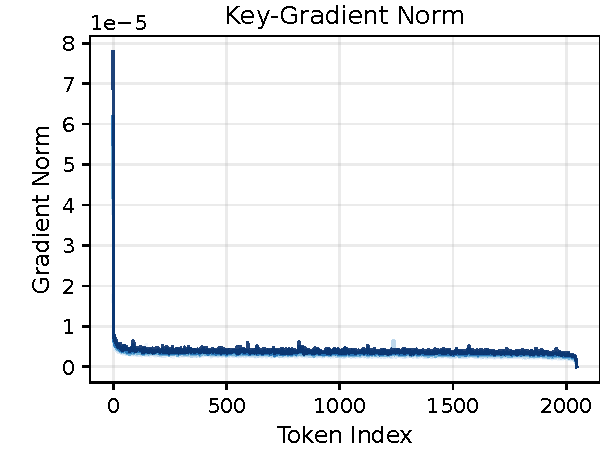
\includegraphics[width=0.3\textwidth]{pics/03B_baseline/LINE_Dk_over_tokens.pdf}
    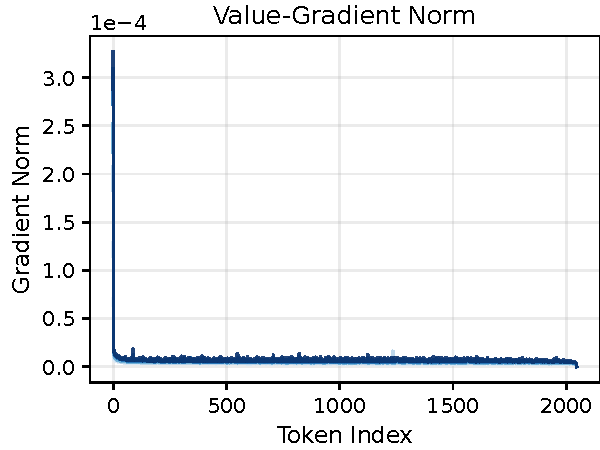
\includegraphics[width=0.3\textwidth]{pics/03B_baseline/LINE_Dv_over_tokens.pdf}
    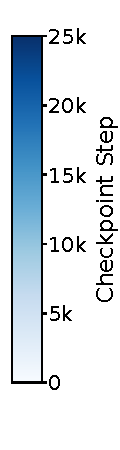
\includegraphics[width=0.06\textwidth]{pics/03B_baseline/line_steps.pdf}
    \caption{
    Token-wise gradient norms of QKV across training checkpoints.
    Top row: 0.1B model; bottom row: 0.3B model.
    From left to right: gradient norms of query, key, and value as functions of token position, averaged over layers.
    In both scales, key and especially value gradients exhibit a pronounced spike at token 0.
    }\label{fig:qkv_grads_over_tokens}
\end{figure}

To analyze the structure of gradient sinks, we further break down the attention block gradients into query, key, and value pathways.
For each pathway, the statistics are averaged over layers.
Figure~\ref{fig:qkv_grads_over_tokens} shows a clear and highly structured asymmetry.
On the key and value pathways, the gradient norm exhibits a pronounced spike at the first token across checkpoints, after which it drops rapidly and remains relatively flat over most of the sequence.
Moreover, the value-path spikes are observed to be substantially larger than the key-side ones.
The query pathway looks qualitatively different and its token-wise gradient profile is comparatively flat across most positions.
In fact, the query gradient at the first token is exactly zero under causal masking.

Thus, 
these observations establish the central empirical fact of this section:
in pretrained Transformer models, the sink token is not only a forward attention sink but also a backward gradient sink.

\subsection{Theoretical results}\label{subsec:theory_as_to_gs}

We next show that the link of AS and GS is not just an empirical regularity.
This subsection focuses exclusively on the most central theoretical framework. 
Supplementary theoretical results and complete proofs are provided in Appendix~\ref{app:theory}.

Let $g_t := \nabla_{y_t}\mathcal{L} = W_O^\top \nabla_{o_t}\mathcal{L}$ denote the upstream gradient. Recall that $M_s$ and $S_s$ in \eqref{eq:sink_mass} denote the attention column mass and its second moment, respectively. Then by direct computation we have the exact V-side gradients $\nabla_{v_s}\mathcal{L} = \sum\nolimits_{t=1}^{T} a_{ts} g_t$.
This identity exposes that the gradient on $v_s$ is an attention-weighted sum of all upstream gradients whose outputs read value from token $s$. If many later tokens attend to token $s$, then many later gradients also pass through $v_s$. To formalize this intuition, we adopt a mean-plus-noise decomposition $g_t = \mu + \varepsilon_t$ for stochastic gradients~\cite{mandt2017sgd, mccandlish2018noise}.

\begin{theorem}[V-side gradient control by sink statistics]\label{thm:v_second_moment_main}
Assume $g_t = \mu + \varepsilon_t$, where $\mathbb{E}[\varepsilon_t]=0$, $\mathrm{Tr}(\mathrm{Cov}(\varepsilon_t)) \le \sigma^2$ for all $t$, and $|\mathrm{Tr}(\mathrm{Cov}(\varepsilon_t,\varepsilon_{t'}))| \le \rho$ for all $t \ne t'$. Then we have
\[
M_s^2\|\mu\|_2^2
\le
\mathbb{E}\big[\|\nabla_{v_s}\mathcal{L}\|_2^2\big]
\le
M_s^2\|\mu\|_2^2 + \sigma^2 S_s + \rho(M_s^2 - S_s).
\]
\end{theorem}

Theorem~\ref{thm:v_second_moment_main} shows that sink structure provides a natural and quantitatively explicit route to value-path gradient concentration. 
The same derivation also yields exact query/key-path gradients, see Propositions~\ref{prop:k-exact-app} and~\ref{prop:q-exact-app} in Appendix~\ref{app:theory}.
The crucial asymmetry is that K-side gradients aggregate column-wise just as V-side ones, while Q-side gradients are row-local.
These match our measurements that the sink token shows strong value/key gradient concentration but no special query-path advantage.

\section{Gradient reshaping by massive activations}
\label{sec:pressure_reshape}

Section~\ref{sec:as_to_gs} established that attention sinks induce a pronounced gradient sink on the first token. The next question is why this matters for optimization. The key issue is that such concentration creates a persistent local optimization burden that must be reshaped before it can be propagated through a deep residual network. If the sink token repeatedly receives much larger branch-local gradients than other tokens, one would expect either disproportionately strong local updates or a distortion of gradient transport along the residual stream. From this perspective, GS is a pressure that the network must absorb while keeping training in a stable regime. 

This section examines how the localized gradient pressure is reshaped and whether the observed MA pattern aligns with a concrete gradient-compression mechanism in pre-norm architectures.
For each layer of a checkpoint, we compare the activation norms of the attention branch input $\|h_{\mathrm{in}}^\ell\|$, against three ratios defined in \eqref{eq:ratios_attn}: $\mathrm{Bloat}^{\mathrm{attn},\ell}$, $\mathrm{Compress}^{\mathrm{attn},\ell}$, and $\mathrm{Change}^{\mathrm{attn},\ell}$.
The same measurements for the MLP branch are deferred to Appendix~\ref{app:mlp_reshaping}.

\begin{figure}[tb]
    \centering
    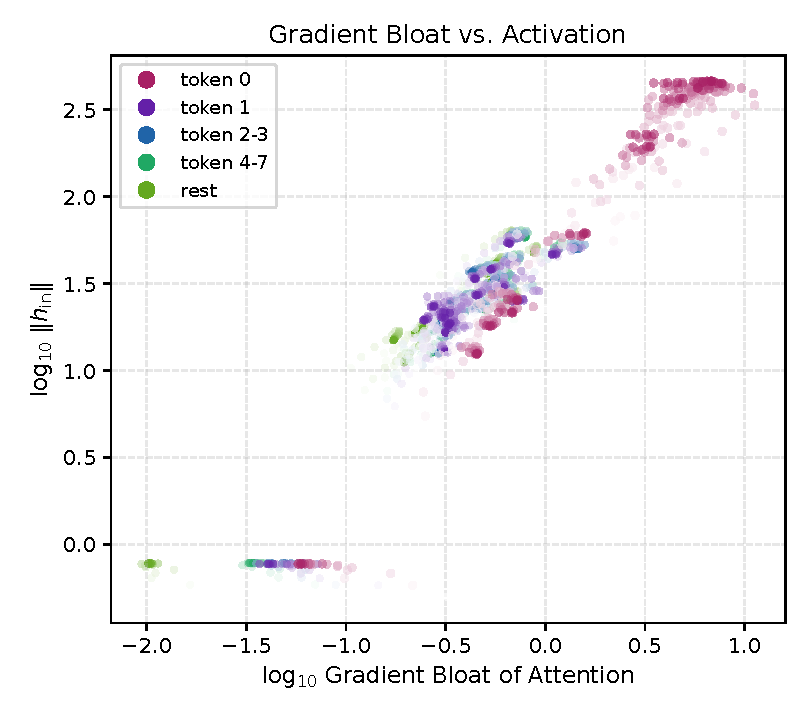
\includegraphics[width=0.3\linewidth]{pics/01B_baseline/Ea3_Bloat.pdf}
    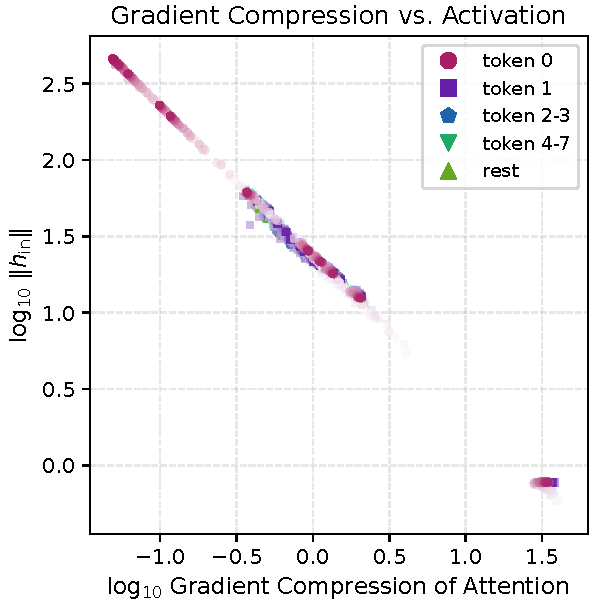
\includegraphics[width=0.3\linewidth]{pics/01B_baseline/Ea1_compress.pdf}
    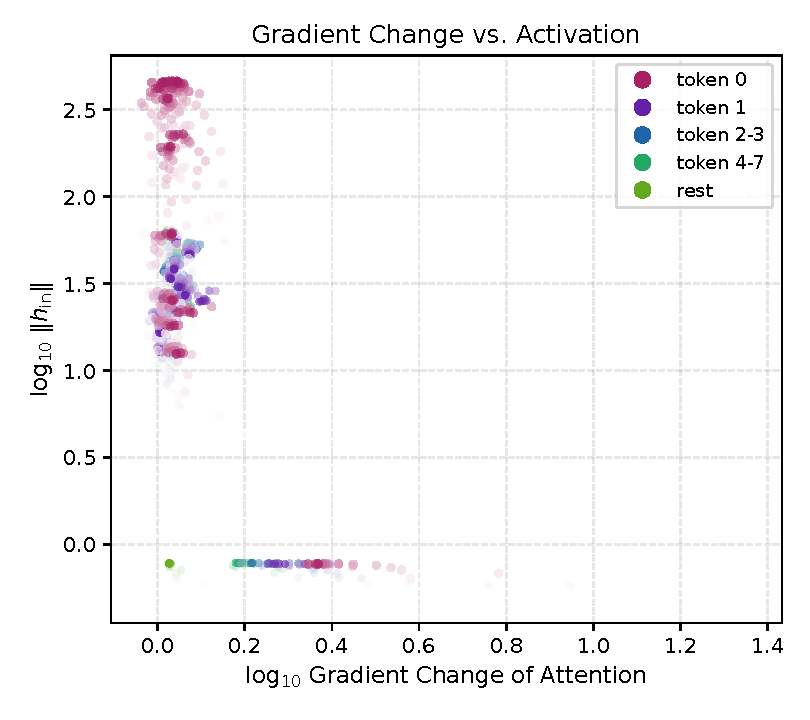
\includegraphics[width=0.3\linewidth]{pics/01B_baseline/Ea4_Change.pdf}
    \includegraphics[width=0.06\linewidth]{pics/01B_baseline/scatter_group_steps.pdf}
    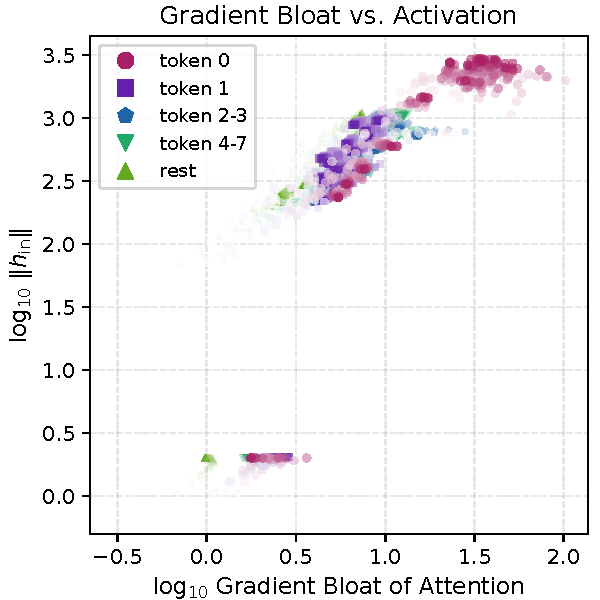
\includegraphics[width=0.3\linewidth]{pics/03B_baseline/Ea3_Bloat.pdf}
    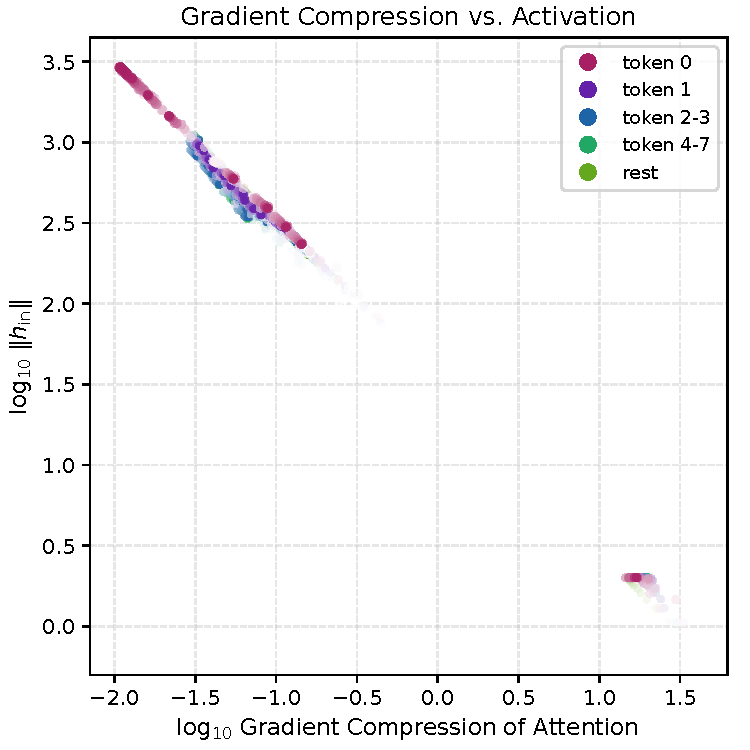
\includegraphics[width=0.3\linewidth]{pics/03B_baseline/Ea1_compress.pdf}
    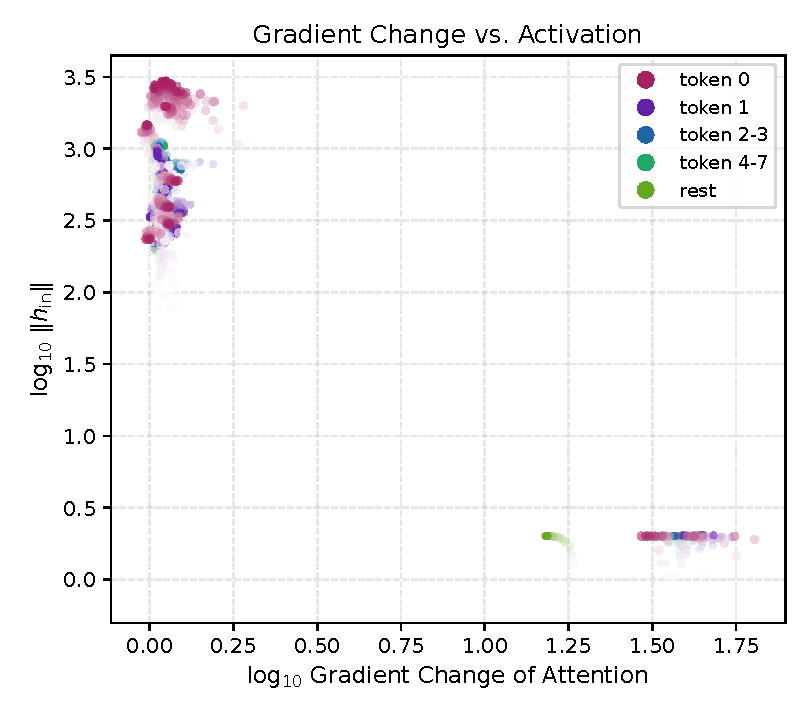
\includegraphics[width=0.3\linewidth]{pics/03B_baseline/Ea4_Change.pdf}
    \includegraphics[width=0.06\linewidth]{pics/03B_baseline/scatter_group_steps.pdf}
    \caption{
    Scatter plots relating gradient reshaping to input activation norms of Attention block. Top row: 0.1B model; bottom row: 0.3B model.
    From left to right: $\log_{10}\mathrm{Bloat}^{\mathrm{attn}}$ vs.\ $\log_{10}\|h_{\mathrm{in}}\|$, 
    $\log_{10}\mathrm{Compress}^{\mathrm{attn}}$ vs.\ $\log_{10}\|h_{\mathrm{in}}\|$, and
    $\log_{10}\mathrm{Change}^{\mathrm{attn}}$ vs.\ $\log_{10}\|h_{\mathrm{in}}\|$.
    Each point is colored by token group (token 0, token 1, tokens 2--3, tokens 4--7, and the rest early tokens 8--15).
    Large-activation points of token 0 occupy the high-bloat regime. Compression exhibits an approximately linear inverse relationship with activation scale. The net residual-level change remains concentrated near $\log_{10}1=0$ except for a small set of first-layer points.
    }\label{fig:attn_scatter_main}
\end{figure}

Figure~\ref{fig:attn_scatter_main} shows that these three ratios play sharply different roles.
The scatter plots are colored by token groups.
In the left panel, large-activation points concentrate in the high-bloat regime dominated by token 0, while the remaining tokens occupy a much milder regime.
This means that the gradient norms of the sink token are not merely large in an absolute sense but are most strongly amplified in the attention branch.

The middle panel shows that $\mathrm{Compress}^{\mathrm{attn}}$ lies on an almost linear trend with slope $-1$, indicating that RMSNorm-mediated attenuation is closely aligned with activation scale.

The right panel explains why this alignment matters.
Although $\mathrm{Bloat}^{\mathrm{attn}}$ can become very large on the first token, the corresponding $\mathrm{Change}^{\mathrm{attn}}$ values remain concentrated near $\log_{10}1 = 0$, except for some points located in the lower-right corner from the first layer.
Thus the localized gradient pressure revealed by $\mathrm{Bloat}^{\mathrm{attn}}$ is largely reshaped into a regime compatible with stable residual propagation.
This observation is consistent with the broader literature, in which residual networks are thought to remain optimizable at depth as the signal propagation stays appropriately close to identity, rather than drifting into systematic explosion or collapse~\cite{he2016deep,zhang2019fixup,liu2020understanding,bachlechner2021rezero,wang2024deepnet}.

The empirical alignment between massive activations and strong compression is not accidental.
It follows from a basic property of RMSNorm.

\begin{theorem}[Activation-dependent compression under RMSNorm]\label{thm:rms_compress_main}
Denote $y=\mathrm{RMSNorm}(x) = \gamma \odot \frac{x}{\rms(x)}$ with $\rms(x)=\sqrt{\frac{1}{d}\|x\|_2^2+\epsilon}$, and let $g_y=\nabla_y\mathcal{L}$ be the upstream gradient at the RMSNorm output.
Then we have $\nabla_x\mathcal{L}=J_{\mathrm{rms}}(x)^\top g_y$, and the Jacobian satisfies $\|J_{\mathrm{rms}}(x)\|_{\mathrm{op}} \le \frac{\|\gamma\|_\infty}{\rms(x)}$.
\end{theorem}

The proof is deferred to Appendix~\ref{app:theory}.
The theorem formalizes a key intuition that larger incoming activation norm provides a direct route to stronger local attenuation of backpropagated gradients.

In total, we observe that localized gradients are not merely large but selectively processed by pre-norm computation.
In the attention branch, the sink token exhibits strong branch-local amplification, strong normalization-induced attenuation, and only limited net gradient change.
These results support the mechanism whereby massive activations attenuate localized gradient pressure through RMSNorm.

\section{V-scale: a value-path gradient valve}
\label{sec:vscale}

The previous sections suggest a concrete and testable prediction of our mechanism. If massive activations are primarily responses to localized gradient pressure, then reducing that pressure should weaken MA even when attention sinks are largely preserved. More practically, such an intervention would help improve robustness under quantization, as MA is empirically associated with inference fragility. % TODO: maybe reference
This section implements this prediction.

Several recent architectural variants mitigate extreme phenomena like MA and AS by changing the Softmax function, inserting gates, or modifying normalization structure~\cite{zuhri2025softpick,qiu2025gated,bu2025valuestategated,sun2026spike}.
While valuable, these changes significantly alter the forward geometry and therefore do not cleanly isolate and test the specific prediction of our hypothesis. 
Here we instead seek a mathematically transparent modification that remains close to the original Llama-like model.

The value path is the natural target channel for two reasons.
First, our backward observations in Section~\ref{sec:as_to_gs} confirm that value-path gradient norms of the sink token are several times larger than key-path ones. 
Second, prior studies have repeatedly reported that sink tokens tend to have unusually small value norms~\cite{guo2025activedormant,su2025kvsink,bu2025valuestategated}.
We observe the same pattern and are inspired by this useful structural prior: if sink values are already small, a radial transform depending on $\|v\|_2$ can selectively target sink tokens.

\subsection{Definition and design intuition}

For each attention head, after the standard value projection and before value aggregation, we replace $y_t = \sum\nolimits_{j\le t} a_{tj} v_j$ by
\[
\hat v_j = \phi(\|v_j\|_2^2)\, v_j,
\quad
\phi(r)=\frac{r}{r+C},
\quad
\hat y_t = \sum\nolimits_{j\le t} a_{tj} \hat v_j,
\]
where $C>0$ is a scale parameter. We call this modification \emph{V-scale}, as illustrated in Figure~\ref{fig:architecture}.



This map is chosen to satisfy three design desiderata.
First, it does not affect the attention weights that depend only on $Q$ and $K$.
Second, it is close to identity when $\|v_j\|_2^2 \gg C$, because $\phi(r) \to 1$ as $r\to\infty$.
Third, it strongly suppresses small-norm values, since $\phi(r) \approx r/C$ when $r\ll C$.
This makes V-scale a targeted modification rather than a uniform shrinkage.
Moreover, because those small-norm tokens already contribute little through the forward value sum, the induced forward perturbation is limited exactly in the regime where the gradient intervention is strongest.

\begin{wrapfigure}[12]{r}{0.36\linewidth}
	\centering
	\vspace{-10px}
	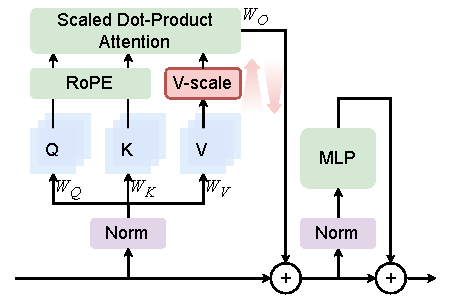
\includegraphics[width=1\linewidth]{pics/vscale_architecture.pdf}\caption{Schematic of V-scale inside a pre-norm Transformer block.}
	\label{fig:architecture}
\end{wrapfigure}

In practice we use a scaled reparameterization $C_{\ell,h} = (d_{\mathrm{head}}\sigma)^2\lambda^{\ell,h}$, where $\sigma=0.02$ is the standard deviation employed for initializing the weight matrix in \texttt{LlamaForCausalLM} baselines and $\lambda^{\ell,h}$ is either fixed to $1$ or learned as $\lambda^{\ell,h}=\exp(\theta_{\ell,h})$.
% 为什么这样初始化
This learnable version introduces only one parameter per layer and per head, which is negligible relative to the total parameter count. We implement this learnable version in this work.

As expected, the backward behavior of V-scale is analyzable.
Let $r=\|v\|_2^2$ and $\hat v=\phi(r)v$ with $\phi(r)=r/(r+C)$.
Then the Jacobian of the V-scale map $v\mapsto \hat v$ is $J_{\phi}(v) = \phi(r) I + \frac{2C}{(r+C)^2} vv^\top$, which has eigenvalue $\lambda_\perp(r)=\frac{r}{r+C}$ on the $(d_{\mathrm{head}}-1)$-dimensional subspace orthogonal to $v$, and eigenvalue $\lambda_\parallel(r) = \frac{r^2+3Cr}{(r+C)^2}$ along the radial direction $v$. Thus if $\|v\|_2^2\ll C$ for the sink token, the value-path backward signal is strongly attenuated.

\begin{remark}
The gradient arriving at the token representation after RMSNorm is not a pure value-path quantity but the sum of the $Q$, $K$, and $V$ paths $\nabla_{\widetilde h_s^\ell}\mathcal{L} = W_Q^\top \nabla_{q_s^\ell}\mathcal{L} + W_K^\top \nabla_{k_s^\ell}\mathcal{L} + W_V^\top \nabla_{v_s^\ell}\mathcal{L}$.
Therefore, modifying only the value path cannot completely eliminate gradient sinks.
Our goal is to show that once the dominant value-path pressure is supplied with an alternative valve, the optimizer no longer needs to build the same degree of MA.
\end{remark}

\subsection{Experiments}

We train V-scale models using the same data, optimizer, and model configurations as the corresponding baselines. These models can achieve slightly lower validation losses compared to the baselines. 
While evaluated at relatively modest scales, these results establish that intervening on gradient sinks via V-scale does not disrupt the fundamental trainability of the architecture.

\begin{figure}[tb]
    \centering
    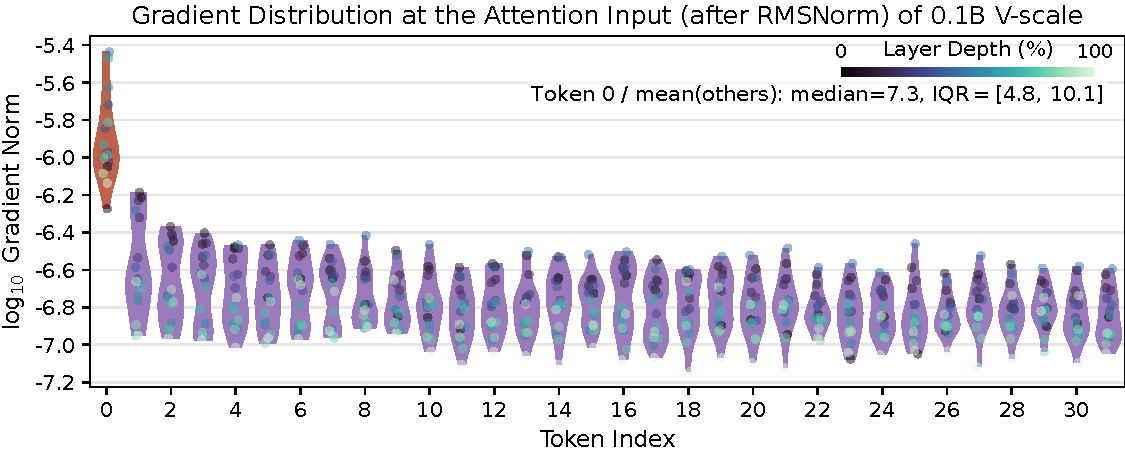
\includegraphics[width=0.48\textwidth]{pics/01B_vscale_learn/violin.pdf}
    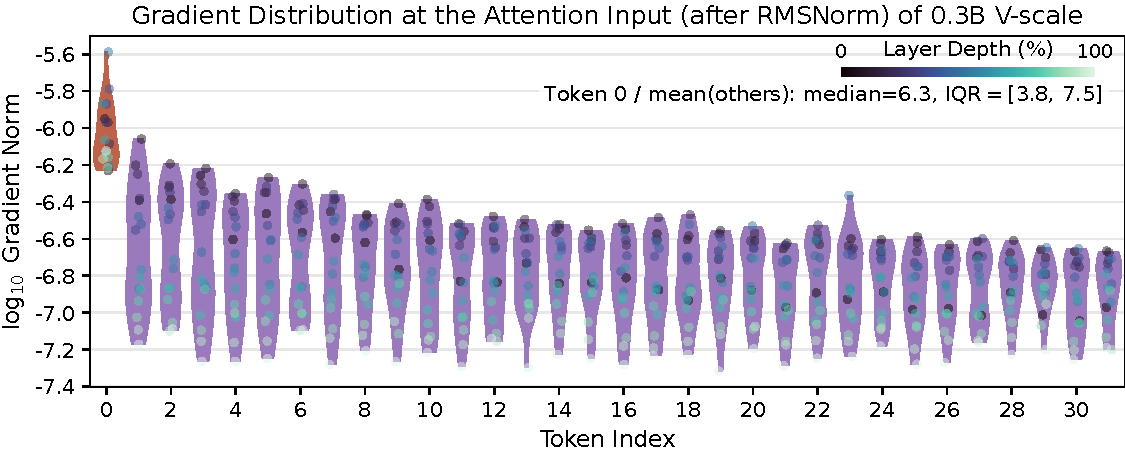
\includegraphics[width=0.48\textwidth]{pics/03B_vscale_learn/violin.pdf}
    \caption{
    Gradient sink phenomenon in V-scale models. Each panel plots the token-wise distribution of $\log_{10}\|\nabla_{\widetilde h_t^{\ell}}\mathcal L\|_2$ at the post-RMSNorm attention input. Token 0 is highlighted while other early tokens share a common color. The median and IQR of $R_{GS}^{\ell}$ are also reported. Both scales show that gradient sinks remain present but are substantially weaker than the baselines, with the median token-0-to-rest ratio dropping to roughly $7.3$ and $6.3$ in the 0.1B and 0.3B V-scale models, respectively.
    }\label{fig:vscale-gs}
\end{figure}

\begin{figure}[tb]
    \centering
    % 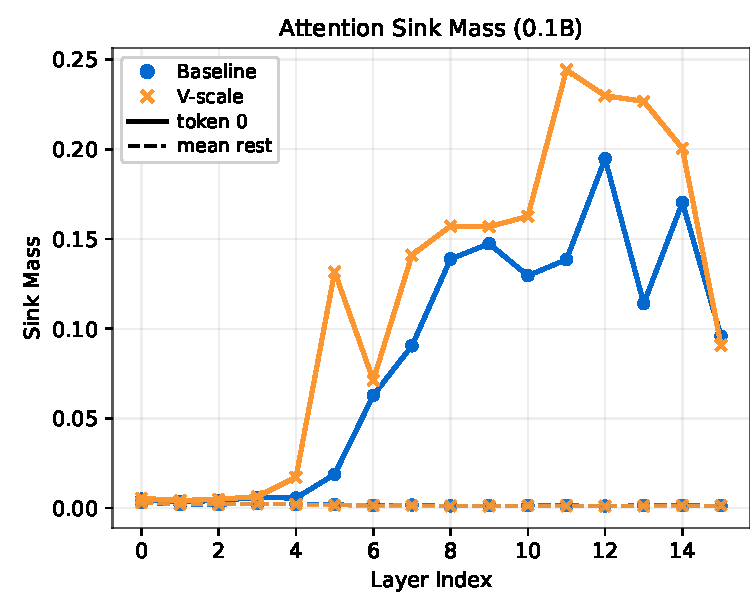
\includegraphics[width=0.24\linewidth]{pics/compare/01B_AS_mass_final_compare.pdf}
    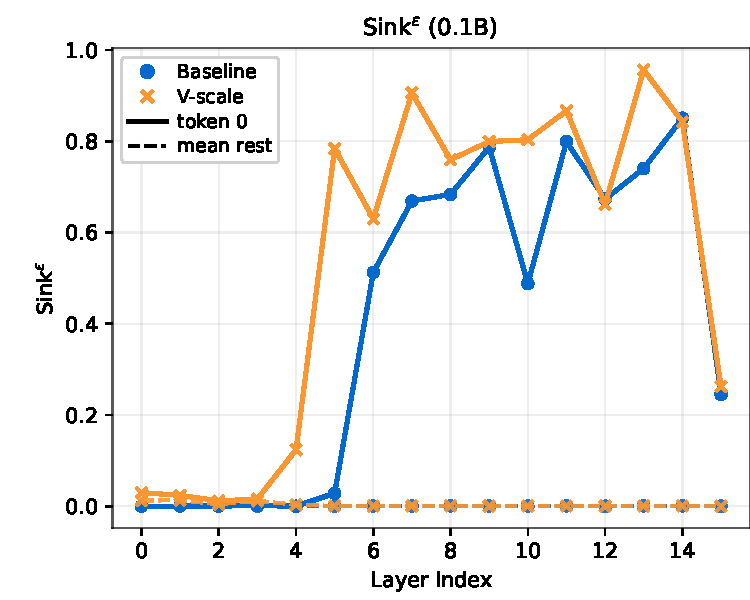
\includegraphics[width=0.24\linewidth]{pics/compare/01B_AS_eps_final_compare.pdf}
    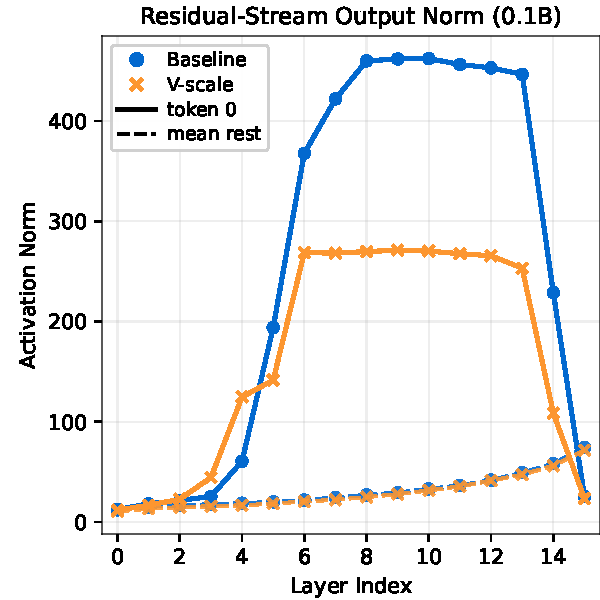
\includegraphics[width=0.24\linewidth]{pics/compare/01B_MA_x_out_final_compare.pdf}
    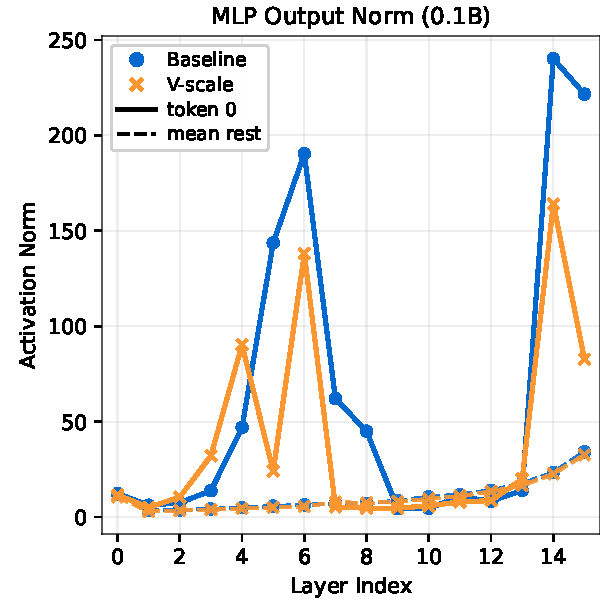
\includegraphics[width=0.24\linewidth]{pics/compare/01B_MA_mlp_out_final_compare.pdf}
    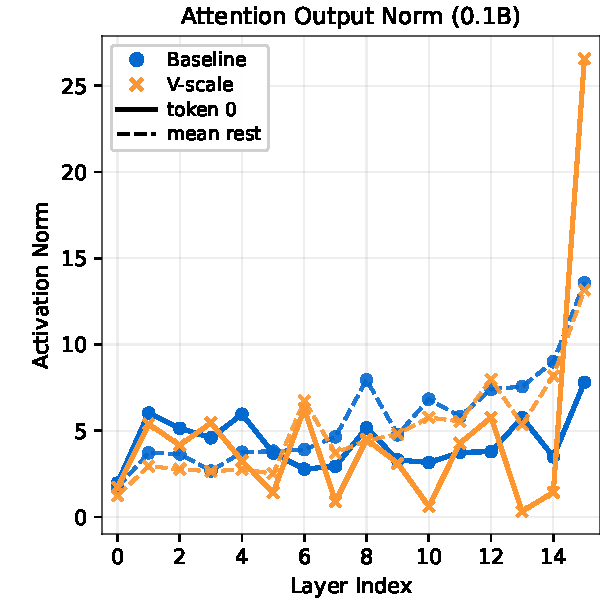
\includegraphics[width=0.24\linewidth]{pics/compare/01B_MA_attn_out_final_compare.pdf}
    \\
    % 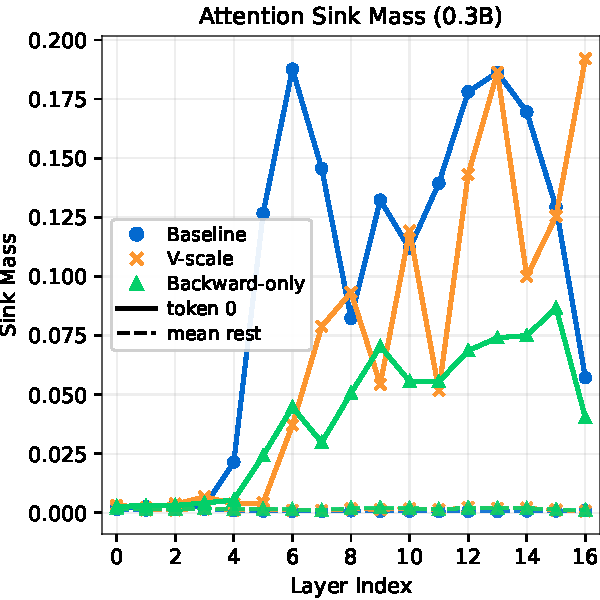
\includegraphics[width=0.24\linewidth]{pics/compare/03B_AS_mass_final_compare.pdf}
    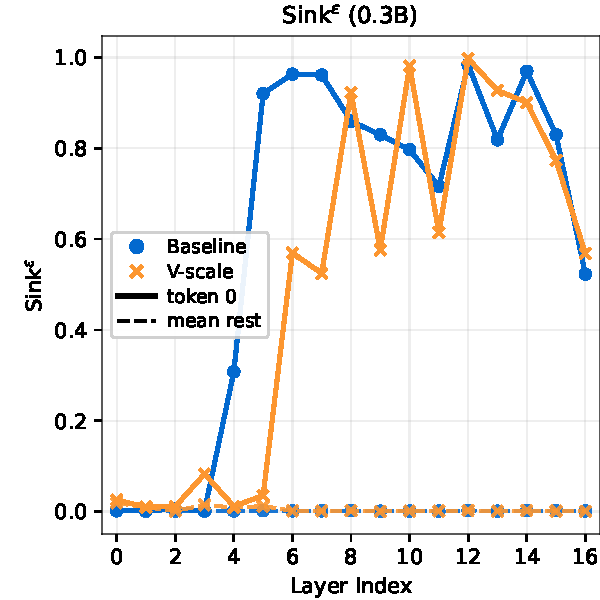
\includegraphics[width=0.24\linewidth]{pics/compare/03B_AS_eps_final_compare.pdf}
    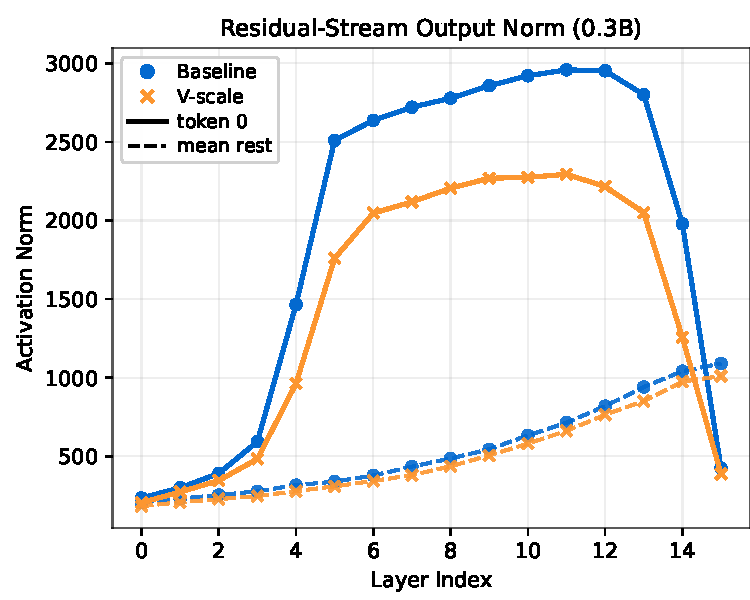
\includegraphics[width=0.24\linewidth]{pics/compare/03B_MA_x_out_final_compare.pdf}
    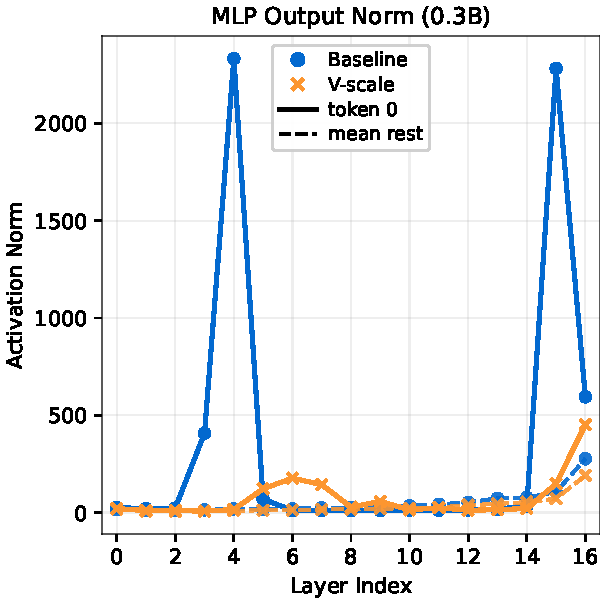
\includegraphics[width=0.24\linewidth]{pics/compare/03B_MA_mlp_out_final_compare.pdf}
    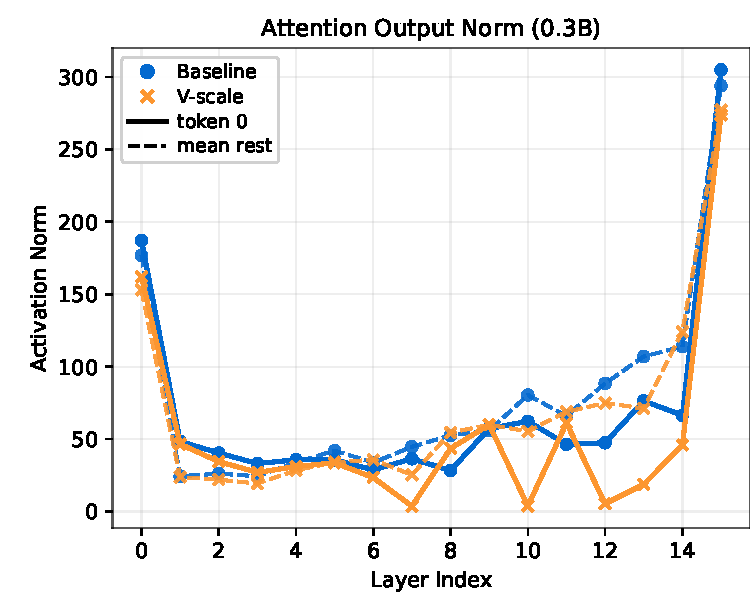
\includegraphics[width=0.24\linewidth]{pics/compare/03B_MA_attn_out_final_compare.pdf}
    \caption{
    Forward phenomena in baseline and V-scale models.
    Top row: 0.1B models; bottom row: 0.3B models.
    % From left to right: attention sink mass, thresholded sink rate, residual-stream output norm, and MLP output norm.
    From left to right: thresholded sink rate, residual-stream output norm, MLP output norm, and Attention output norm.
    We compare the first token with the mean over the rest early tokens (positions 1--15).
    Across both scales, V-scale largely preserves sink behavior while reducing the activation norms of token 0, with the larger reduction appearing in MLP outputs.
    }\label{fig:vscale_as_ma_compare}
\end{figure}

\paragraph{Mechanism verification}
We re-measure gradient sinks using the same definition as in Figure~\ref{fig:gs-definition}. Figure~\ref{fig:vscale-gs} shows that the gradient sink remains clearly present but is substantially weaker. In our measurements, the median $R_{GS}^{\ell}(0)$ defined in~\eqref{eq:gs_def} drops from the baseline values ($14.8$ and $9.0$) to roughly $7.3$ and $6.3$ in the 0.1B and 0.3B V-scale models, respectively. This is exactly the expected outcome of a partial intervention on the value-path gradient.

Moreover Figure~\ref{fig:vscale_as_ma_compare} compares baseline and V-scale models on the most relevant token-wise forward observables for AS and MA: thresholded Sink Rate $\mathrm{Sink}_s^{\epsilon,\ell}$ in \eqref{eq:sink_rate}, residual-stream output norm, MLP output norm, and Attention output norm.

The results are consistent across both model scales. On the AS metrics, V-scale preserves strong sink behavior and in several layers even slightly strengthens it. In contrast, on the MA metrics, the residual-stream and MLP output norms of token 0 are clearly reduced relative to the baselines. 
The attention output norms of token 0 are also reduced, which is expected since V-scale directly contracts the value path. However, this direct attenuation is modest in magnitude compared with the reduction in the learned MLP spikes. 
Overall, these observations match the qualitative prediction of our mechanism: by providing an additional gradient valve on the dominant value path, V-scale reduces the pressure for the model to realize MA through large MLP outputs, rather than merely shrinking the attention output.

\paragraph{Downstream performance}
To verify that the suppression of massive activations via V-scale does not compromise fundamental capabilities, we evaluate our 0.3B models on a suite of downstream tasks. We further assess robustness under post-training quantization (PTQ), since massive activations manifest as extreme outliers that are known to severely degrade quantized inference. We employ the LM Evaluation Harness~\cite{eval-harness} and compare models under standard \texttt{bfloat16} precision as well as five PTQ protocols spanning diverse design points: naive symmetric INT8 quantization (Naive W8A8)~\cite{gholami2021survey}, SmoothQuant (W8A8)~\cite{xiao2023smoothquant}, BitsAndBytes (W4A16)~\cite{dettmers2023qlora}, GPTQ (W4A16)~\cite{frantar2023optq}, and AWQ (W4A16)~\cite{lin2024awq}, where W$x$A$y$ denotes $x$-bit weight and $y$-bit activation quantization.

Table~\ref{tab:quant_03b_main} reports language modeling perplexity and zero-shot reasoning accuracy. Under bfloat16 and all quantization settings, the V‑scale model performs on par with or even surpasses the baseline, confirming that substantially reducing activations does not compromise its representational capacity. 

To further investigate the impact on long-range attention allocation, we conduct the Needle-in-a-Haystack (NIAH) retrieval test across context lengths from 512 to
2048 tokens. Table~\ref{tab:quant_03b_niah} reports retrieval accuracy under bfloat16 and the same five PTQ protocols used above.
Under full-precision bfloat16, V-scale slightly outperforms the baseline at the longest context (87.9\% vs. 82.5\%), indicating that
suppressing massive activations does not impair the ability to route attention over long ranges.
The advantage becomes substantially more pronounced under quantization. With the exception of naive W8A8, V-scale consistently outperforms the baseline across all other PTQ settings at context length 2048, with absolute gains ranging from +3.0\% (GPTQ) to +25.9\% (BitsAndBytes W4A16). 
These results are consistent with the hypothesis that massive activations disproportionately harm quantized representations, particularly for longer contexts.

Taken together, these results demonstrate that the reduction in massive activations achieved by V-scale translates into concrete downstream robustness. The quantization-friendly activation profile preserves long-range retrieval fidelity, providing practical evidence that controlling gradient sinks yields more deployment-ready models.

\section{Conclusions}

In this work, we revisit the relationship between attention sinks and massive activations from the perspective of backpropagation.
Our empirical and theoretical results suggest that the connection between the two is not merely a forward-pass correlation, but is mediated by a backward mechanism: under causal masking, attention sinks can induce concentrated gradient pressure on the sink token, forming gradient sinks, and massive activations emerge as an adaptive response to this localized pressure in pre-norm Transformers.
To test this hypothesis, we introduce V-scale, a value-path intervention that selectively modulates backpropagated gradients.
Across models, we find that V-scale preserves attention sinks but suppresses massive activations, illustrating that these two phenomena can be separated once gradient sinks are controlled.
Across model sizes, V-scale preserves attention sinks but suppresses massive activations, showing that AS and MA can be separated once GS is controlled. Robustness under quantization is also improved.

Taken together, our findings suggest that some phenomena in large language models may not be best understood purely as forward functional structures but a reflection to how optimization adapts to architectural constraints in order to maintain stable gradient transport. We believe this gradient-regulation perspective may be useful for future designs of normalization, attention mechanisms, and training-time interventions that aim to preserve the benefits of sink structure while reducing its costs.

\paragraph{Limitations}
This work has some limitations.
First, our study is restricted to Llama-like dense language models. It remains unclear whether and to what extent the same mechanism transfers to other settings, such as mixture-of-experts architectures or multimodal Transformers.
Second, our analysis is primarily a mechanism study of why MA can be useful once GS exists, rather than a complete account of how AS and MA are learned throughout optimization.
These limitations are left for future work.

\bibliographystyle{plain}
\bibliography{neurips_2026}

\clearpage
\appendix

%\end{document}

\iffalse
\section{Quanming}

\subsection{Difference}

\begin{table}[ht]
	\centering
	\small
	\setlength\tabcolsep{1pt}
	\begin{tabular}{C{1.5cm} C{5cm} C{2.5cm} C{4.5cm}}
		\toprule
		\textbf{Work} & \textbf{Main idea} & \textbf{Overlap with ours} & \textbf{Key difference / our contribution} \\ 
		\midrule
		
		Bondarenko et al. (2023) 
		& Activation outliers arise from heads implementing ``no-op'' behavior under softmax; propose clipped softmax and gating 
		& Optimization-based explanation of extreme activations 
		& Does not identify token-level gradient concentration or an explicit mediator linking AS and MA \\ \midrule
		
		Sun et al. (2024) 
		& Massive activations are widespread and act as bias terms affecting attention 
		& Links MA with attention behavior 
		& Primarily forward/functional view; no backward-pass mediator \\ \midrule
		
		Gu et al. (2025) 
		& Empirical study of when attention sinks emerge 
		& Strong characterization of AS 
		& No mechanism connecting AS to MA \\ \midrule
		
		Guo et al. (2025) 
		& Training-time mutual reinforcement explains extreme-token phenomena 
		& Closest prior mechanistic work 
		& No explicit formulation of gradient sinks or RMSNorm-based response \\ \midrule
		
		Barbero et al. (2025) 
		& First-token attention avoids over-mixing 
		& Functional explanation of AS 
		& Does not address MA or gradient dynamics \\ \midrule
		
		Queipo-de-Llano et al. (2026) 
		& Connects attention sinks and compression valleys via massive activations 
		& Links AS and MA 
		& Treats MA as primary driver; we instead identify GS as mediator \\ \midrule
		
		Sun et al. (2026) 
		& AS/MA co-occurrence is a pre-norm architectural artifact 
		& Alternative explanation of coupling 
		& Focuses on architecture; we focus on training dynamics \\ \midrule
		
		Softpick (2025) 
		& Modifies softmax to remove AS and MA 
		& Intervention on same phenomena 
		& Alters forward geometry; not a targeted causal test \\ \midrule
		
		Gated Attention (2025) 
		& Uses output gating to mitigate extreme-token behavior 
		& Large-scale mitigation 
		& Not designed to isolate causal mechanism \\ \midrule
		
		VGA (2025) 
		& Value-state gating based on gradient analysis 
		& Closest intervention method 
		& Does not isolate a minimal mechanism preserving AS while suppressing MA \\ \midrule
		
		\textbf{Ours} 
		& AS induces GS; MA arises as RMSNorm-mediated response; V-scale intervention 
		& --- 
		& Identifies GS as explicit mediator and provides sink-preserving causal validation \\ 
		
		\bottomrule
	\end{tabular}
	\caption{Comparison with existing works on attention sinks, massive activations, and mitigation methods.}
	\label{tab:related}
\end{table}

\subsection{Contributions}

\begin{itemize}[leftmargin=*]
	\item 
	We identify gradient sinks as an explicit backward-pass mediator of extreme-token behavior in causal, pre-norm Transformers.
	
	\item
	We reinterpret massive activations, within RMSNorm pre-norm models, as a local gradient-compression response to sink-induced pressure.
	
	\item
	We propose V-scale, a lightweight value-path intervention that largely preserves attention sinks while reducing massive activations, providing a targeted causal test of the GS hypothesis.
\end{itemize}

\subsection{Organization}

\begin{figure}[H]
	\centering
	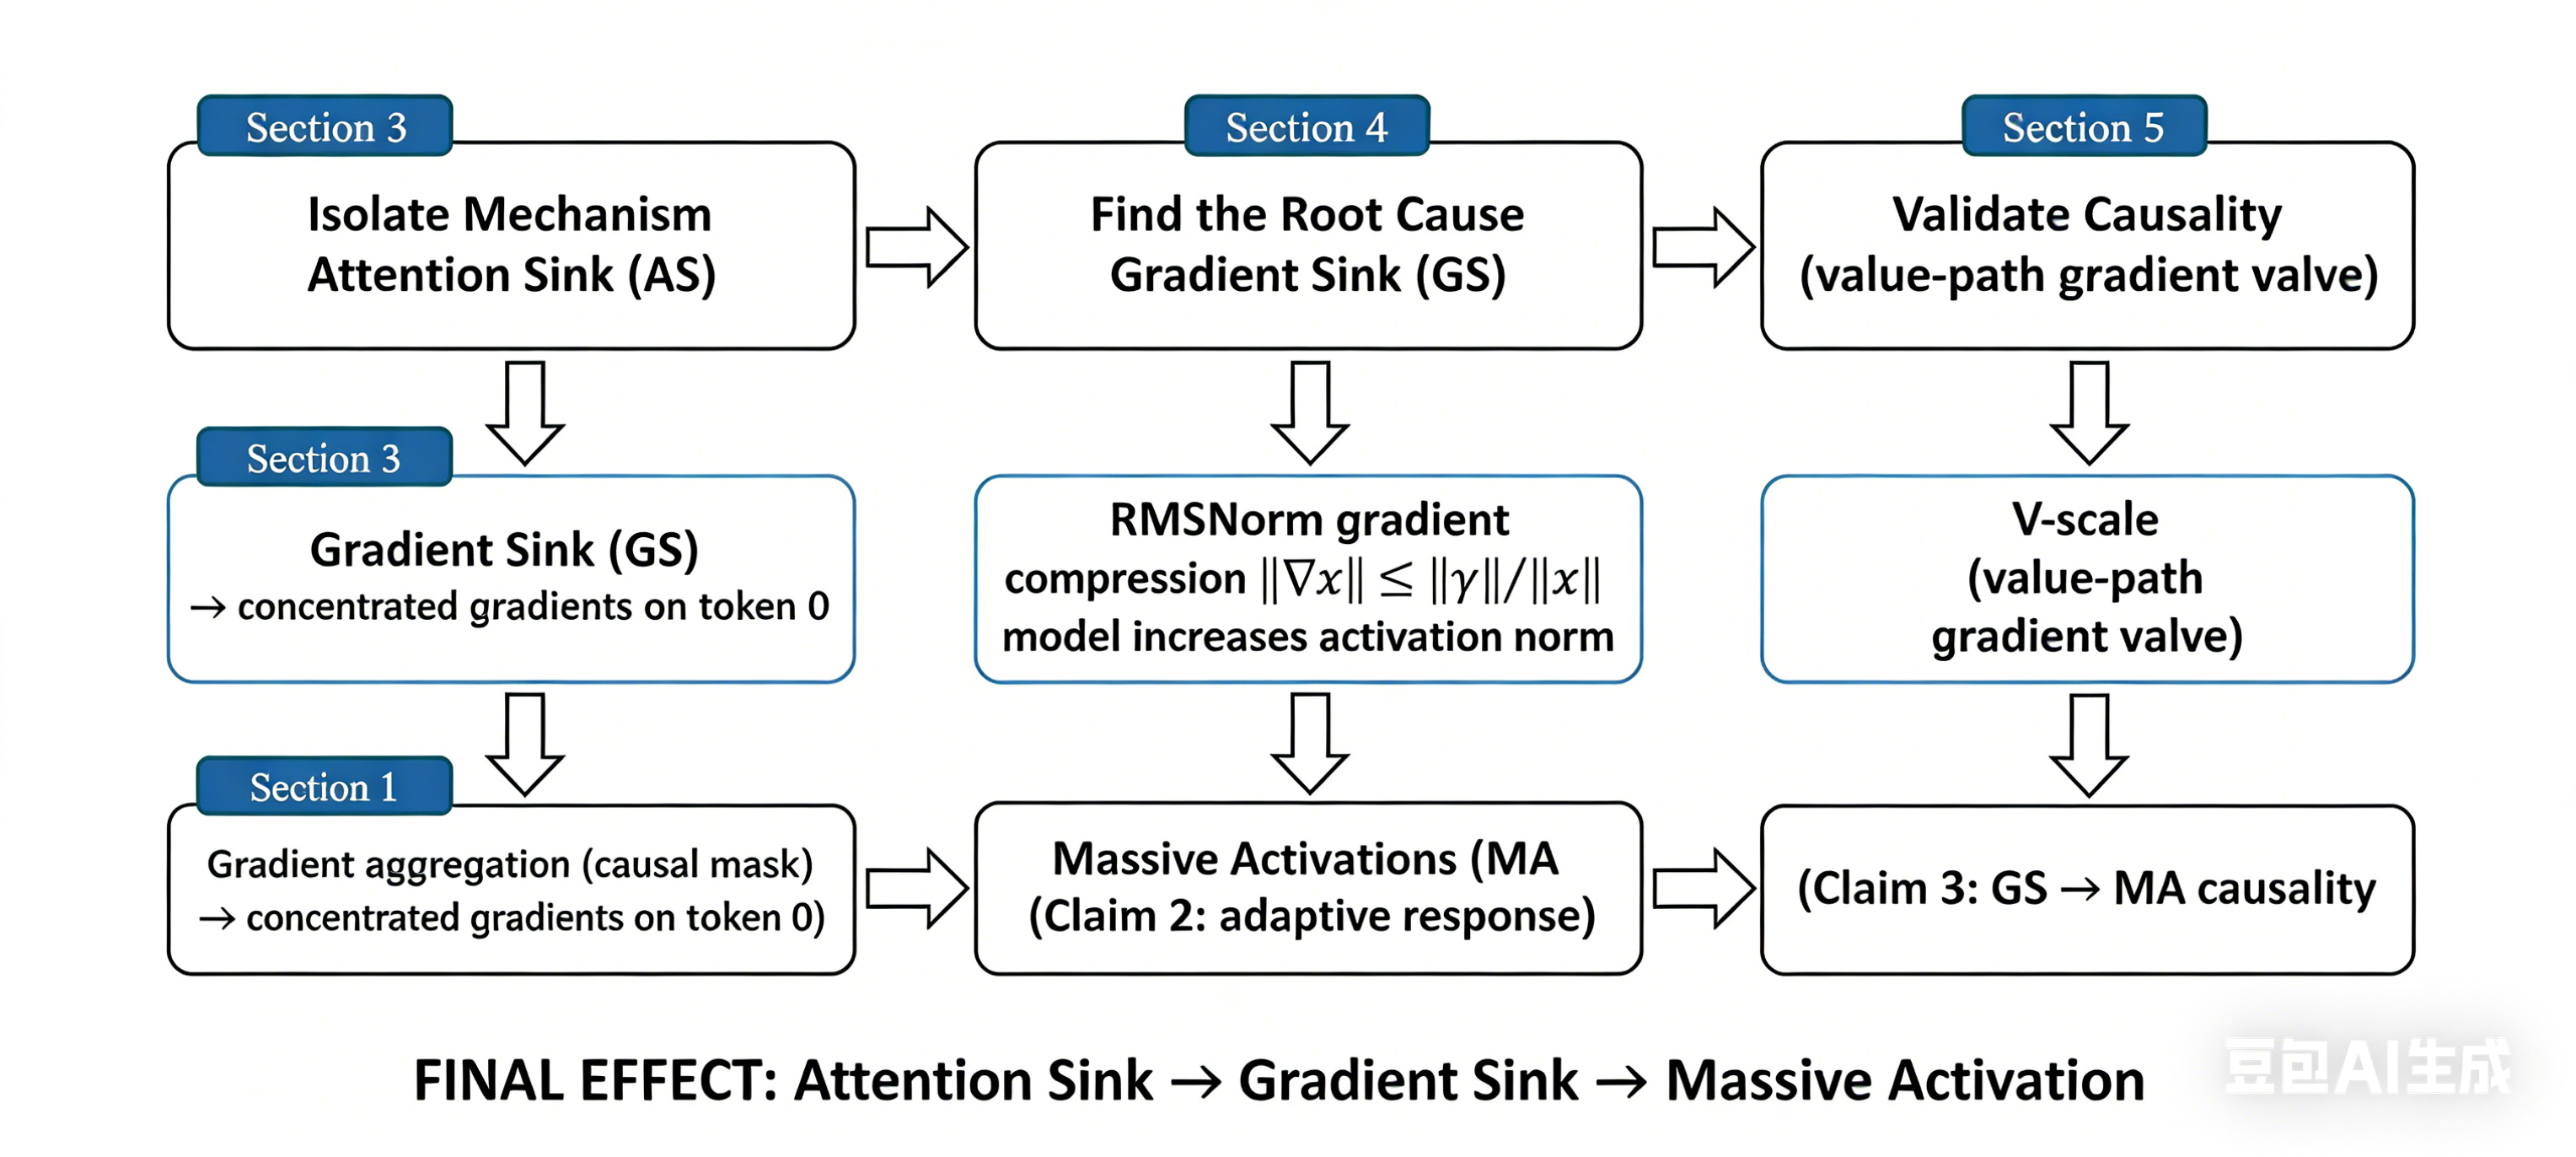
\includegraphics[width=1.0\linewidth]{pics/org}
\end{figure}

\subsection{Introduction}

Transformer-based language models exhibit a striking and persistent behavior: a small number of tokens—most notably the first token—attract disproportionate attention from the rest of the sequence, while simultaneously developing unusually large activation magnitudes. These extreme-token phenomena, commonly referred to as attention sinks and massive activations, have been widely observed across model scales and architectures, and have significant implications for long-context modeling, numerical stability, and efficient deployment.

Despite their prevalence, the origin of these phenomena remains poorly understood. Existing explanations largely focus on the forward computation, interpreting attention sinks as functional structures such as context anchors or no-op attention heads, and massive activations as representational artifacts or bias-like terms. However, these perspectives leave a fundamental question unanswered: \textbf{why does optimization consistently produce such coupled and extreme behaviors?} This question is particularly puzzling in modern pre-norm Transformers, where both attention and feed-forward layers operate on normalized representations. In such architectures, forward computation depends primarily on representation direction rather than magnitude, suggesting that large activation norms should play a limited role. Yet in practice, massive activations not only emerge but tightly co-occur with attention sinks throughout training. This apparent mismatch indicates that forward-pass explanations alone are insufficient.

In this work, we revisit this problem from the perspective of training dynamics and uncover a previously overlooked mechanism. We show that attention sinks not only dominate the forward pass, but also induce concentrated gradient flow during backpropagation, forming what we term gradient sinks. Under causal masking, gradients from many tokens aggregate onto the sink token, creating localized gradient pressure that is highly asymmetric across token positions. We further demonstrate that, in pre-norm architectures, massive activations arise as an adaptive response to this imbalance: through normalization, larger activation norms attenuate backpropagated gradients, effectively reshaping the gradient flow to maintain stable optimization. This establishes a causal chain from forward attention structure to backward gradient concentration and activation growth.

To validate this mechanism, we introduce V-scale, a lightweight modification that selectively regulates value-path gradients without altering attention weights. Empirically, V-scale preserves attention sinks while significantly suppressing massive activations, providing direct evidence that gradient sinks act as the mediator between the two phenomena. Taken together, our findings suggest that extreme-token behaviors in Transformers are not merely forward artifacts, but are governed by the structure of gradient flow during training, offering a novel lens for understanding and controlling optimization in large language models.

\clearpage

\fi

\section{Model and training configuration}\label{app:config}

Table~\ref{tab:config} summarizes the training configurations used in our experiments.
Unless otherwise specified, all models are decoder-only Transformers with RMSNorm, RoPE positional encoding, SwiGLU feed-forward blocks, and causal self-attention. All training runs were implemented in PyTorch using NVIDIA A100 GPUs (80GB). During preprocessing, documents are packed by inserting \texttt{<eos>} as the separator, without introducing dedicated \texttt{<bos>}.

\begin{table}[h]
    \centering
    \caption{Training configuration. }\label{tab:config}
    \begin{tabular}{p{0.25\linewidth}p{0.15\linewidth}p{0.15\linewidth}p{0.15\linewidth}}
        \toprule
        Item & 0.1B runs & 0.3B runs & 1B runs \\
        \midrule
        \emph{Model} & & & \\
        total parameters & $\sim$101M & $\sim$291M & $\sim$1.04B \\
        vocab size & 50257 & 50257 & 50257 \\
        hidden layers & 16 & 16 & 18 \\
        hidden size & 512 & 1024 & 2048 \\
        attention heads & 8 & 8 & 16 \\
        key/value heads & 8 & 4 & 8 \\
        head dimensions & 64 & 128 & 128 \\
        intermediate size & 1408 & 2816 & 5504 \\
        RMSNorm $\epsilon$ & 1e-5 & 1e-5 & 1e-5 \\
        RoPE base & 10000 & 10000 & 10000 \\
        \midrule
        \emph{Optimizer} & & \\
        optimizer & AdamW & AdamW & AdamW \\
        AdamW $\beta_1$ & 0.9 & 0.9 & 0.9 \\
        AdamW $\beta_2$ & 0.95 & 0.95 & 0.95 \\
        AdamW $\epsilon$ & 1e-8 & 1e-8 & 1e-8 \\
        weight decay & 0.1 & 0.1 & 0.1 \\
        gradient clipping norm & 1.0 & 1.0 & 1.0 \\
        max learning rate & 5e-4 & 1e-3 & 1e-3 \\
        min learning rate & 5e-5 & 1e-4 & 1e-4 \\
        \midrule
        \emph{Training} & & \\
        learning rate schedule & cosine decay & cosine decay & cosine decay \\
        total steps & 20000 & 20000 & 25000 \\
        warmup steps & 1000 & 1000 & 1000 \\
        context length & 1024 & 2048 & 2048 \\
        batch size & 512 & 512 & 512 \\
        tokens per step & 0.52M & 1.05M & 1.05M \\
        total tokens & 10.49B & 20.97B & 26.21B \\
        training data & C4 & C4 & C4 \\
        \bottomrule
    \end{tabular}
\end{table}


\section{Additional empirical results}\label{app:empirical}

\subsection{Supplementary results for gradient reshaping}\label{app:mlp_reshaping}

This subsection provides the gradient-reshaping measurements in Section~\ref{sec:pressure_reshape} for the MLP branch. 
The left panel of Figure~\ref{fig:mlp_scatter_main} shows that $\mathrm{Bloat}^{\mathrm{mlp}}$ is much less dominated by token 0 than in the attention branch.
Thus, the MLP branch does not appear to be the primary location where localized pressure is generated.
By contrast, the middle panel again shows a tight alignment between activation norms and compression as observed in Attention blocks. The right panel also shows that $\mathrm{Change}^{\mathrm{mlp}}$ remains concentrated near $\log_{10}1=0$.

\begin{figure}[tb]
    \centering
    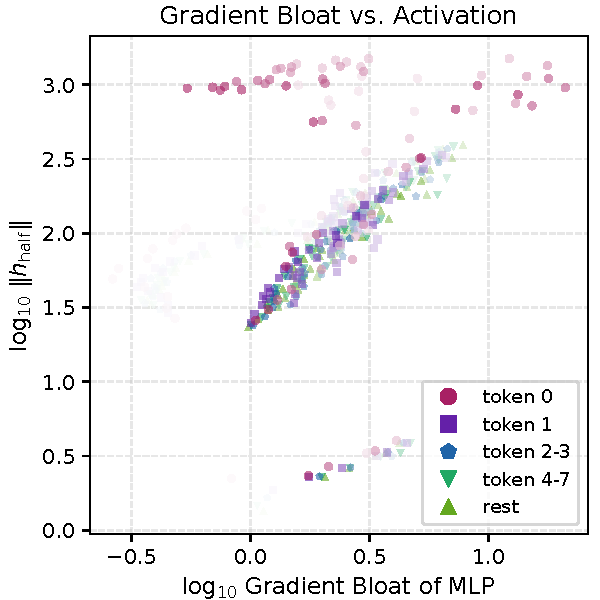
\includegraphics[width=0.3\linewidth]{pics/01B_baseline/Em3_Bloat.pdf}
    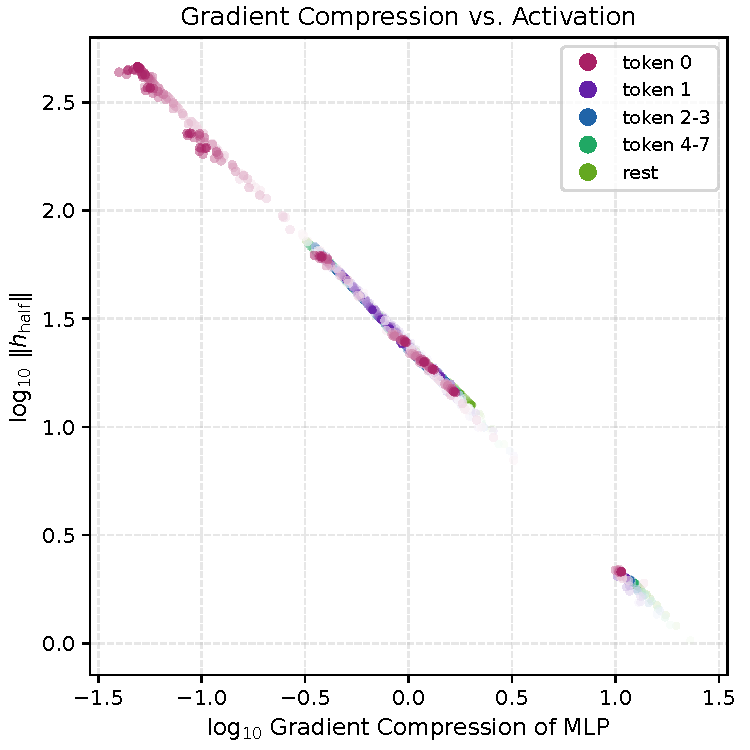
\includegraphics[width=0.3\linewidth]{pics/01B_baseline/Em1_compress.pdf}
    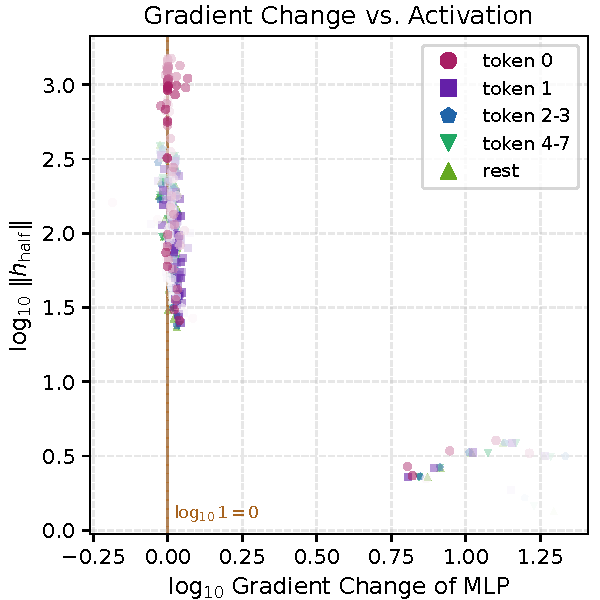
\includegraphics[width=0.3\linewidth]{pics/01B_baseline/Em4_Change.pdf}
    \includegraphics[width=0.06\linewidth]{pics/01B_baseline/scatter_group_steps.pdf}
    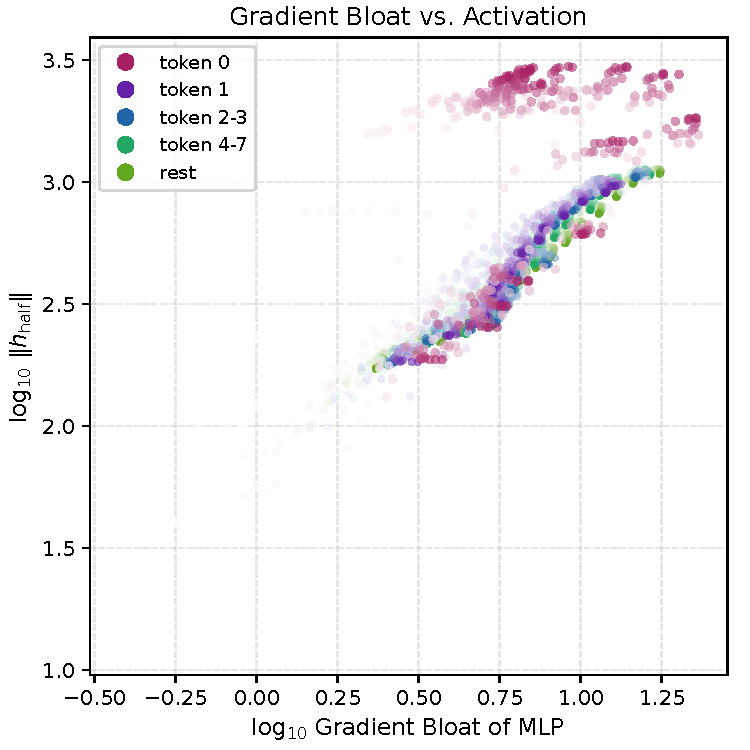
\includegraphics[width=0.3\linewidth]{pics/03B_baseline/Em3_Bloat.pdf}
    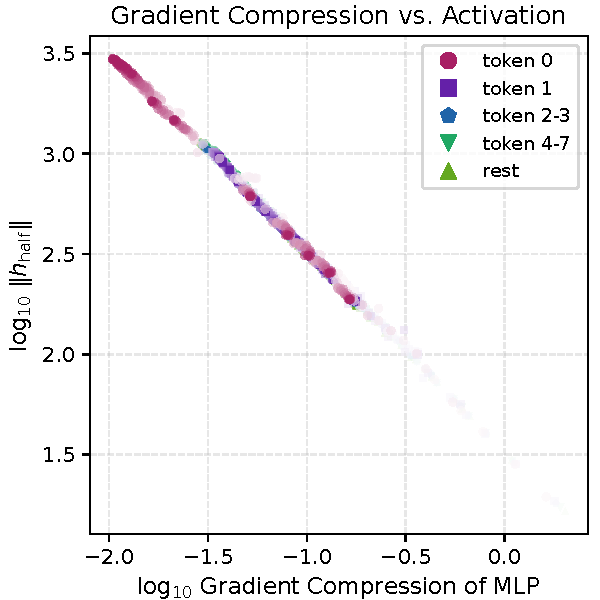
\includegraphics[width=0.3\linewidth]{pics/03B_baseline/Em1_compress.pdf}
    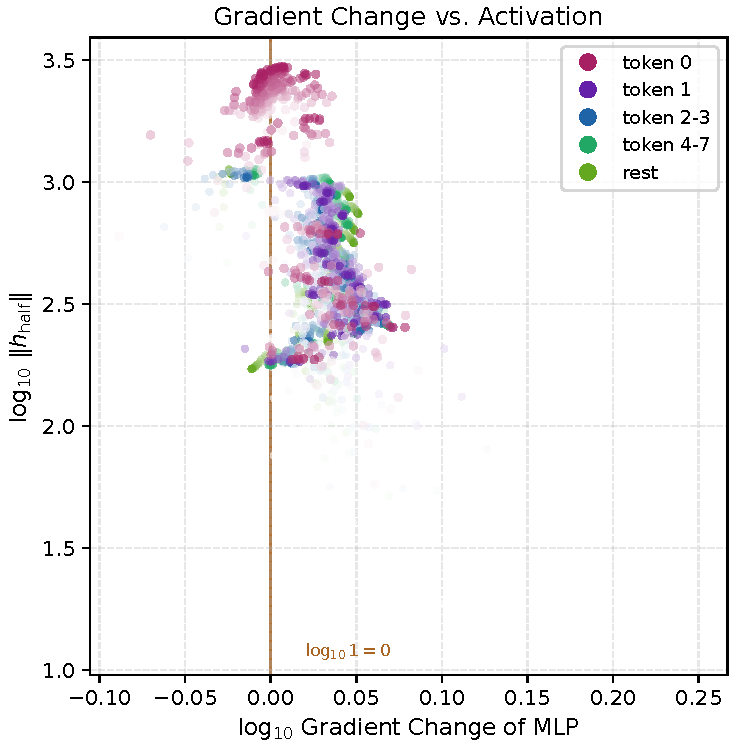
\includegraphics[width=0.3\linewidth]{pics/03B_baseline/Em4_Change.pdf}
    \includegraphics[width=0.06\linewidth]{pics/03B_baseline/scatter_group_steps.pdf}
    \caption{
    Scatter plots relating gradient reshaping to input activation norms of MLP block. Top row: 0.1B model; bottom row: 0.3B model.
    From left to right: $\log_{10}\mathrm{Bloat}^{\mathrm{mlp}}$ vs.\ $\log_{10}\|h_{\mathrm{half}}\|$, 
    $\log_{10}\mathrm{Compress}^{\mathrm{mlp}}$ vs.\ $\log_{10}\|h_{\mathrm{half}}\|$, and
    $\log_{10}\mathrm{Change}^{\mathrm{mlp}}$ vs.\ $\log_{10}\|h_{\mathrm{half}}\|$.
    Each point is colored by token group (token 0, token 1, tokens 2--3, tokens 4--7, and the rest early tokens 8--15).
    Compared with the attention branch, token 0 is less dominant in MLP bloat, while compression again aligns tightly with activation scale and net change remains close to identity.
    }\label{fig:mlp_scatter_main}
\end{figure}

\subsection{Supporting observations for V-scale design}

Figure~\ref{fig:value_state_drain} reports the value-state norms in baseline models. These observations support the design intuition of V-scale: sink tokens tend to have relatively small value norms, making radial contraction on the value path selective rather than uniform.

\begin{figure}[tb]
    \centering
    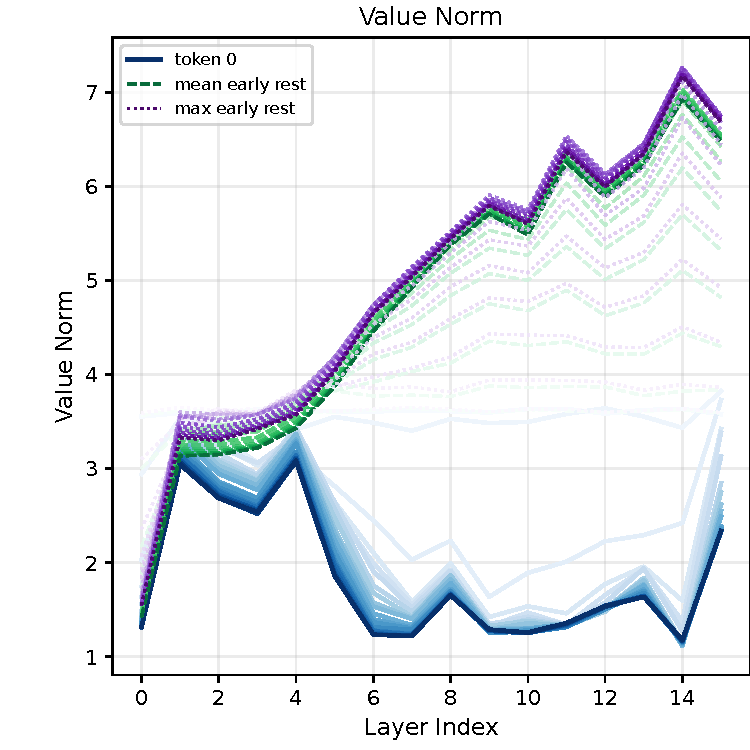
\includegraphics[width=0.3\linewidth]{pics/01B_baseline/V_norm_compare.pdf}
    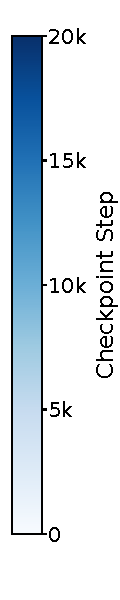
\includegraphics[width=0.06\linewidth]{pics/01B_baseline/extreme_steps.pdf}
    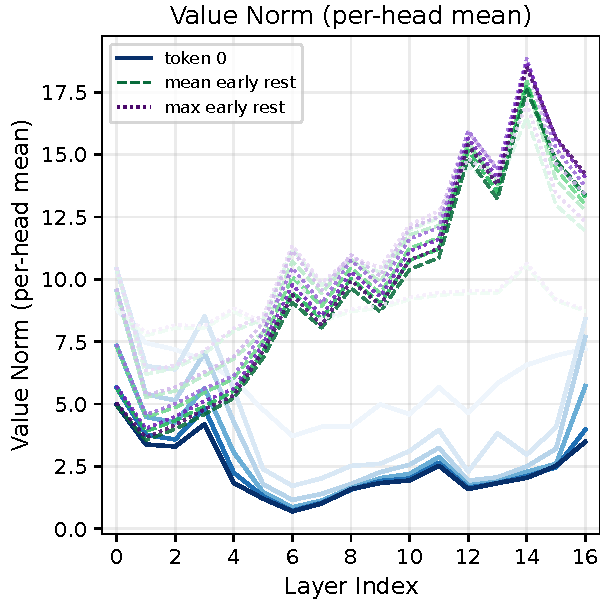
\includegraphics[width=0.3\linewidth]{pics/03B_baseline/V_norm_compare.pdf}
    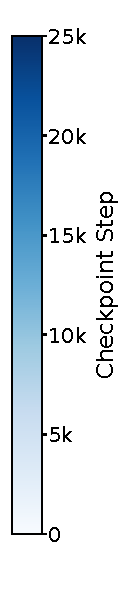
\includegraphics[width=0.06\linewidth]{pics/03B_baseline/extreme_steps.pdf}
    \caption{
    Value state norms in baseline models.
    Left: 0.1B model; right: 0.3B model.
    The ``early rest'' tokens refer to positions 1--15.
    Sink tokens tend to have relatively small value norms compared with the other early tokens.
    }\label{fig:value_state_drain}
\end{figure}

\subsection{Validation losses}

Figure~\ref{fig:validation_loss} shows validation losses of baseline and V-scale models, verifying that the proposed modification remains trainable and reaches comparable optimization quality.

\begin{figure}[tb]
    \centering
    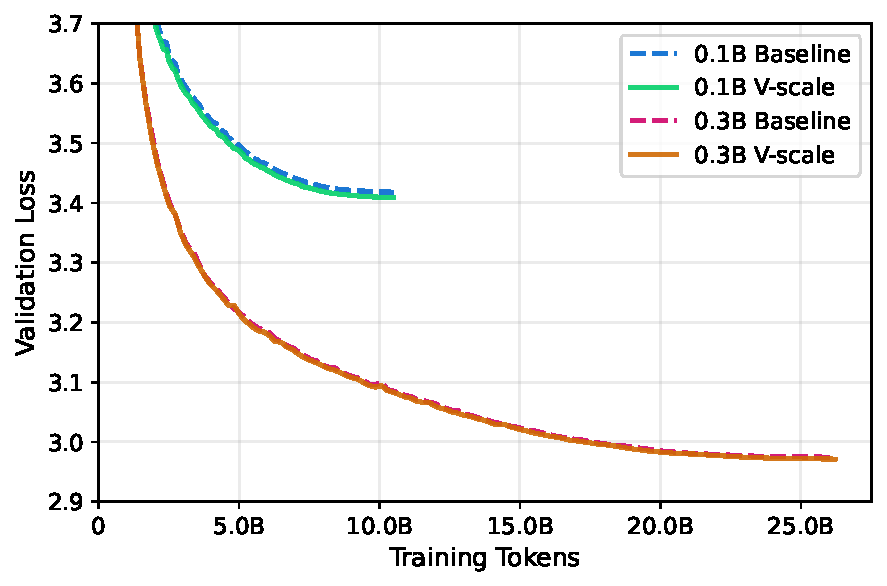
\includegraphics[width=0.5\linewidth]{pics/compare/loss_comparison.pdf}
    \caption{
    Validation losses of baseline and V-scale models.
    }\label{fig:validation_loss}
\end{figure}

\subsection{Downstream tasks}



\begin{table}[h]
    \centering
    \caption{}%\label{}
    \resizebox{\linewidth}{!}{
	\setlength\tabcolsep{2pt}
    \begin{tabular}{llcccccccccccc}
        \toprule
        Model & Quantization & Wiki ppl & Lambada ppl & Lambada acc & ARC-C & ARC-E & BoolQ & COPA & HellaSwag & OBQA & PIQA & SCIQ & WinoGrande \\
        \midrule
        Baseline & bfloat16 & 22.84 & 15.27 & 43.28 & 24.91 & 47.98 & 51.38 & 69.00 & 51.59 & 31.40 & 72.52 & 69.90 & 54.22 \\
        V-scale & bfloat16 & 22.83 & 15.91 & 43.37 & 27.05 & 47.47 & 56.27 & 70.00 & 51.29 & 32.80 & 71.49 & 69.30 & 53.28 \\
        Baseline & SmoothQuant & 23.17 & 16.61 & 43.02 & 25.26 & 47.47 & 50.92 & 67.00 & 51.49 & 30.80 & 72.47 & 69.00 & 55.17 \\
        V-scale & SmoothQuant & 23.01 & 16.58 & 43.14 & 26.11 & 46.76 & 55.57 & 69.00 & 51.13 & 32.40 & 71.00 & 68.30 & 54.46 \\
        Baseline & BNB & 23.49 & 16.40 & 42.73 & 25.00 & 47.43 & 54.19 & 72.00 & 51.59 & 31.40 & 73.01 & 69.20 & 55.56 \\
        V-scale & BNB & 23.40 & 15.86 & 43.55 & 27.56 & 47.05 & 55.96 & 74.00 & 51.29 & 32.80 & 71.27 & 69.50 & 54.14 \\
        Baseline & GPTQ & 23.21 & 15.70 & 43.26 & 25.77 & 48.48 & 52.54 & 68.00 & 51.61 & 31.60 & 72.85 & 69.20 & 54.70 \\
        V-scale & GPTQ & 23.17 & 16.48 & 43.76 & 26.79 & 46.80 & 56.45 & 70.00 & 51.31 & 32.40 & 71.44 & 68.40 & 54.70 \\
        Baseline & AWQ & 23.32 & 16.34 & 42.44 & 25.26 & 48.06 & 53.64 & 68.00 & 51.23 & 30.60 & 72.47 & 69.40 & 54.30 \\
        V-scale & AWQ & 23.36 & 16.95 & 43.06 & 26.71 & 47.10 & 55.96 & 69.00 & 50.88 & 33.20 & 71.65 & 69.10 & 53.51 \\
        \bottomrule
    \end{tabular}
    }
\end{table}



\begin{table}[h]
    \centering
    \caption{niah\_single\_2}%\label{}
    \begin{tabular}{llcccc}
        \toprule
        Model & Quantization & 1024 & 2048 & 4096 & 8192 \\
        \midrule
        \rowcolor[gray]{0.9}\multicolumn{6}{l}{\emph{1B Models}} \\
        Baseline & bfloat16 & $99.96_{\pm 0.09}$ & $98.00_{\pm 0.69}$ & & \\
        V-scale & bfloat16 & $100.00_{\pm 0.00}$ & $97.80_{\pm 0.42}$ & & \\
        Baseline & SmoothQuant & $99.96_{\pm 0.09}$ & $95.92_{\pm 2.09}$ & & \\
        V-scale & SmoothQuant & $100.00_{\pm 0.00}$ & $95.64_{\pm 0.99}$ & & \\
        Baseline & BNB & $99.88_{\pm 0.18}$ & $98.36_{\pm 0.86}$ & & \\
        V-scale & BNB & $100.00_{\pm 0.00}$ & $95.76_{\pm 0.84}$ & & \\
        Baseline & GPTQ & $99.92_{\pm 0.11}$ & $94.64_{\pm 1.56}$ & & \\
        V-scale & GPTQ & $100.00_{\pm 0.00}$ & $96.68_{\pm 0.46}$ & & \\
        Baseline & AWQ & $99.92_{\pm 0.11}$ & $96.56_{\pm 1.24}$ & & \\
        V-scale & AWQ & $100.00_{\pm 0.00}$ & $97.20_{\pm 0.71}$ & & \\
        \midrule
        \rowcolor[gray]{0.9}\multicolumn{6}{l}{\emph{1B Models with YaRN-Extension} (yarn\_factor$=4$)} \\
        Baseline & bfloat16 & $99.84_{\pm 0.22}$ & $98.64_{\pm 0.26}$ & $98.20_{\pm 0.66}$ & $94.20_{\pm 0.75}$ \\
        V-scale & bfloat16 & $99.40_{\pm 0.40}$ & $99.56_{\pm 0.38}$ & $98.32_{\pm 0.41}$ & $99.04_{\pm 0.33}$ \\
        Baseline & SmoothQuant & $99.72_{\pm 0.23}$ & $97.48_{\pm 0.84}$ & $93.24_{\pm 1.21}$ & $88.40_{\pm 1.67}$ \\
        V-scale & SmoothQuant & $98.52_{\pm 0.30}$ & $97.96_{\pm 0.17}$ & $93.72_{\pm 0.63}$ & $96.16_{\pm 0.70}$ \\
        Baseline & BNB & $99.60_{\pm 0.37}$ & $99.20_{\pm 0.37}$ & $98.12_{\pm 0.87}$ & $93.32_{\pm 0.77}$ \\
        V-scale & BNB & $99.76_{\pm 0.17}$ & $99.96_{\pm 0.09}$ & $99.40_{\pm 0.35}$ & $98.52_{\pm 0.50}$ \\
        Baseline & GPTQ & $99.80_{\pm 0.20}$ & $97.32_{\pm 0.61}$ & $96.92_{\pm 0.44}$ & $93.08_{\pm 1.18}$ \\
        V-scale & GPTQ & $99.64_{\pm 0.22}$ & $98.96_{\pm 0.43}$ & $93.52_{\pm 1.14}$ & $97.72_{\pm 0.27}$ \\
        Baseline & AWQ & $99.72_{\pm 0.23}$ & $97.44_{\pm 0.54}$ & $94.60_{\pm 1.02}$ & $90.84_{\pm 1.07}$ \\
        V-scale & AWQ & $96.96_{\pm 0.77}$ & $94.56_{\pm 0.52}$ & $92.36_{\pm 1.40}$ & $98.32_{\pm 0.84}$ \\
        \bottomrule
    \end{tabular}
\end{table}

\begin{table}[h]
    \centering
    \caption{niah\_single\_3}%\label{}
    \begin{tabular}{llcccc}
        \toprule
        Model & Quantization & 1024 & 2048 & 4096 & 8192 \\
        \midrule
        \rowcolor[gray]{0.9}\multicolumn{6}{l}{\emph{1B Models}} \\
        Baseline & bfloat16 & $99.68_{\pm 0.11}$ & $85.48_{\pm 1.24}$ & & \\
        V-scale & bfloat16 & $98.60_{\pm 0.79}$ & $95.60_{\pm 0.95}$ & & \\
        Baseline & SmoothQuant & $99.00_{\pm 0.28}$ & $79.28_{\pm 0.93}$ & & \\
        V-scale & SmoothQuant & $96.00_{\pm 0.84}$ & $88.48_{\pm 0.46}$ & & \\
        Baseline & BNB & $99.32_{\pm 0.18}$ & $79.80_{\pm 1.29}$ & & \\
        V-scale & BNB & $99.44_{\pm 0.48}$ & $96.40_{\pm 0.51}$ & & \\
        Baseline & GPTQ & $99.44_{\pm 0.26}$ & $85.84_{\pm 1.88}$ & & \\
        V-scale & GPTQ & $98.84_{\pm 0.75}$ & $95.84_{\pm 1.13}$ & & \\
        Baseline & AWQ & $99.44_{\pm 0.26}$ & $96.16_{\pm 1.25}$ & & \\
        V-scale & AWQ & $91.96_{\pm 1.01}$ & $85.20_{\pm 1.54}$ & & \\
        \midrule
        \rowcolor[gray]{0.9}\multicolumn{6}{l}{\emph{1B Models with YaRN-Extension} (yarn\_factor$=4$)} \\
        Baseline & bfloat16 & $98.96_{\pm 0.26}$ & $91.56_{\pm 2.03}$ & $79.48_{\pm 1.08}$ & $75.68_{\pm 1.51}$ \\
        V-scale & bfloat16 & $99.08_{\pm 0.70}$ & $94.36_{\pm 1.01}$ & $77.16_{\pm 1.42}$ & $73.52_{\pm 1.10}$ \\
        Baseline & SmoothQuant & $97.00_{\pm 0.82}$ & $80.12_{\pm 2.11}$ & $71.96_{\pm 2.07}$ & $64.00_{\pm 1.38}$ \\
        V-scale & SmoothQuant & $98.56_{\pm 0.84}$ & $84.84_{\pm 1.15}$ & $64.72_{\pm 1.57}$ & $66.92_{\pm 1.20}$ \\
        Baseline & BNB & $98.60_{\pm 0.63}$ & $89.64_{\pm 1.11}$ & $75.68_{\pm 1.14}$ & $75.52_{\pm 2.39}$ \\
        V-scale & BNB & $99.16_{\pm 0.48}$ & $98.64_{\pm 0.46}$ & $82.52_{\pm 0.94}$ & $71.72_{\pm 1.98}$ \\
        Baseline & GPTQ & $98.92_{\pm 0.23}$ & $90.68_{\pm 1.30}$ & $75.72_{\pm 1.32}$ & $73.68_{\pm 0.70}$ \\
        V-scale & GPTQ & $99.36_{\pm 0.57}$ & $94.36_{\pm 0.99}$ & $61.04_{\pm 1.58}$ & $69.20_{\pm 1.97}$ \\
        Baseline & AWQ & $98.76_{\pm 0.52}$ & $96.56_{\pm 0.50}$ & $78.24_{\pm 0.74}$ & $74.20_{\pm 1.83}$ \\
        V-scale & AWQ & $98.24_{\pm 0.75}$ & $87.84_{\pm 1.11}$ & $49.80_{\pm 1.73}$ & $70.56_{\pm 1.98}$ \\
        \bottomrule
    \end{tabular}
\end{table}

\begin{table}[h]
    \centering
    \caption{niah\_multikey\_1}%\label{}
    \begin{tabular}{llcccc}
        \toprule
        Model & Quantization & 1024 & 2048 & 4096 & 8192 \\
        \midrule
        \rowcolor[gray]{0.9}\multicolumn{6}{l}{\emph{1B Models}} \\
        Baseline & bfloat16 & $67.96_{\pm 1.34}$ & $65.04_{\pm 1.09}$ & & \\
        V-scale & bfloat16 & $73.88_{\pm 1.06}$ & $71.64_{\pm 3.46}$ & & \\
        Baseline & SmoothQuant & $64.44_{\pm 1.43}$ & $61.64_{\pm 2.91}$ & & \\
        V-scale & SmoothQuant & $71.64_{\pm 1.44}$ & $69.60_{\pm 2.19}$ & & \\
        Baseline & BNB & $66.16_{\pm 1.68}$ & $61.60_{\pm 1.83}$ & & \\
        V-scale & BNB & $74.04_{\pm 1.65}$ & $70.56_{\pm 2.19}$ & & \\
        Baseline & GPTQ & $66.20_{\pm 1.12}$ & $63.00_{\pm 1.54}$ & & \\
        V-scale & GPTQ & $67.88_{\pm 1.06}$ & $65.56_{\pm 2.25}$ & & \\
        Baseline & AWQ & $63.96_{\pm 2.10}$ & $61.68_{\pm 1.52}$ & & \\
        V-scale & AWQ & $66.84_{\pm 1.75}$ & $67.76_{\pm 3.10}$ & & \\
        \midrule
        \rowcolor[gray]{0.9}\multicolumn{6}{l}{\emph{1B Models with YaRN-Extension} (yarn\_factor$=4$)} \\
        Baseline & bfloat16 & $57.76_{\pm 2.29}$ & $53.88_{\pm 1.42}$ & $48.00_{\pm 2.58}$ & $48.32_{\pm 1.85}$ \\
        V-scale & bfloat16 & $59.28_{\pm 1.77}$ & $59.72_{\pm 2.33}$ & $56.16_{\pm 2.39}$ & $62.00_{\pm 1.88}$ \\
        Baseline & SmoothQuant & $52.44_{\pm 1.84}$ & $49.64_{\pm 1.73}$ & $45.76_{\pm 2.17}$ & $48.96_{\pm 1.89}$ \\
        V-scale & SmoothQuant & $57.92_{\pm 2.26}$ & $57.92_{\pm 1.98}$ & $52.88_{\pm 1.18}$ & $57.64_{\pm 1.28}$ \\
        Baseline & BNB & $54.76_{\pm 2.60}$ & $46.28_{\pm 1.38}$ & $42.72_{\pm 2.96}$ & $47.56_{\pm 2.22}$ \\
        V-scale & BNB & $58.00_{\pm 2.40}$ & $58.40_{\pm 2.20}$ & $55.88_{\pm 1.43}$ & $62.60_{\pm 1.06}$ \\
        Baseline & GPTQ & $56.28_{\pm 1.64}$ & $50.24_{\pm 0.84}$ & $45.20_{\pm 2.81}$ & $46.72_{\pm 1.56}$ \\
        V-scale & GPTQ & $56.68_{\pm 1.36}$ & $57.08_{\pm 0.91}$ & $51.16_{\pm 1.61}$ & $58.96_{\pm 2.20}$\\
        Baseline & AWQ & $54.04_{\pm 1.91}$ & $49.32_{\pm 2.02}$ & $42.52_{\pm 2.98}$ & $47.04_{\pm 2.04}$ \\
        V-scale & AWQ & $59.24_{\pm 1.31}$ & $59.00_{\pm 1.46}$ & $49.64_{\pm 1.95}$ & $58.48_{\pm 2.02}$ \\
        \bottomrule
    \end{tabular}
\end{table}

\section{Additional theoretical results and proofs}\label{app:theory}

This appendix consolidates the supplementary theoretical material used in the main text. Throughout, we fix one layer and one attention head, and use the notation introduced in Section~\ref{sec:prelim}.

\subsection{Exact backpropagation identities}\label{app:theory:exact}

\begin{lemma}[Softmax Jacobian identity]\label{lem:softmax-jacobian-app}
Fix a row $t$ and consider the causal softmax vector $a_t = \mathrm{softmax}(z_t)$ on the support $\{j \le t\}$. Then for any $j,s \le t$,
\[
    \frac{\partial a_{tj}}{\partial z_{ts}} = a_{tj} \bigl(\mathbf{1}_{j=s} - a_{ts}\bigr).
\]
\end{lemma}
\begin{proof}
By definition, we have $a_{tj} = \frac{e^{z_{tj}}}{\sum\nolimits_{\ell \le t} e^{z_{t\ell}}}$. Differentiating with respect to $z_{ts}$ gives
\[
    \frac{\partial a_{tj}}{\partial z_{ts}}
    = \frac{e^{z_{tj}} \mathbf{1}_{j=s} \left(\sum\nolimits_{\ell \le t} e^{z_{t\ell}}\right) - e^{z_{tj}} e^{z_{ts}}}{\left(\sum\nolimits_{\ell \le t} e^{z_{t\ell}}\right)^2}
    = a_{tj} \bigl(\mathbf{1}_{j=s} - a_{ts}\bigr).
\]
\end{proof}

\begin{lemma}[Sensitivity of $y_t$ to a single logit]\label{lem:yt-logit-app}
For fixed $t$ and $s \le t$, we have
\[
    \frac{\partial y_t}{\partial z_{ts}} = a_{ts} (v_s - y_t).
\]
\end{lemma}
\begin{proof}
Using $y_t = \sum\nolimits_{j \le t} a_{tj} v_j$ and Lemma~\ref{lem:softmax-jacobian-app}, we have
\[
    \frac{\partial y_t}{\partial z_{ts}}
    = \sum\nolimits_{j \le t} \frac{\partial a_{tj}}{\partial z_{ts}} v_j
    = \sum\nolimits_{j \le t} a_{tj} (\mathbf{1}_{j=s} - a_{ts}) v_j
    = a_{ts} v_s - a_{ts} \sum\nolimits_{j \le t} a_{tj} v_j
    = a_{ts}(v_s - y_t).
\]
\end{proof}

\begin{proposition}[Exact value-side gradient]\label{prop:v-exact-app}
For any sink index $s$, we have
\[
    \nabla_{v_s} \mathcal{L} = \sum\nolimits_{t=s}^T a_{ts} g_t.
\]
\end{proposition}
\begin{proof}
For fixed $t$, the Jacobian of $y_t$ with respect to $v_s$ is $\frac{\partial y_t}{\partial v_s} = a_{ts} I \mathbb{I}_{s\le t}$. Applying the chain rule from $v_s \to y_t \to L$ yields
\[
    \nabla_{v_s} \mathcal{L}
    = \sum\nolimits_{t=s}^T \left(\frac{\partial y_t}{\partial v_s}\right)^\top \nabla_{y_t} \mathcal{L}
    = \sum\nolimits_{t=s}^T (a_{ts} I)^\top g_t
    = \sum\nolimits_{t=s}^T a_{ts} g_t.
\]
\end{proof}

\begin{proposition}[Exact key-side gradient]\label{prop:k-exact-app}
Define
\[
    \beta_{ts} := \langle g_t, v_s - y_t \rangle.
\]
Then we have
\[
    \nabla_{k_s} \mathcal{L} = \sum\nolimits_{t=1}^T a_{ts} \beta_{ts} \frac{q_t}{\sqrt{d}}.
\]
\end{proposition}
\begin{proof}
The key $k_s$ affects the logits $z_{ts} = \langle q_t, k_s \rangle / \sqrt{d}$ for all $t \ge s$. Since $a_{ts}=0$ when $t<s$, we may sum over all $t$. The chain rule gives
\[
    \nabla_{k_s} \mathcal{L}
    = \sum\nolimits_{t=1}^T \left(\frac{\partial z_{ts}}{\partial k_s}\right)^\top \frac{\partial L}{\partial z_{ts}}.
\]
By $\frac{\partial z_{ts}}{\partial k_s} = \frac{q_t}{\sqrt{d}}$ and Lemma~\ref{lem:yt-logit-app}, we have
\[
    \frac{\partial \mathcal{L}}{\partial z_{ts}}
    = \left\langle \nabla_{y_t} \mathcal{L}, \frac{\partial y_t}{\partial z_{ts}} \right\rangle
    = \langle g_t, a_{ts}(v_s - y_t) \rangle
    = a_{ts} \beta_{ts}.
\]
Substituting these two identities gives the claim.
\end{proof}

\begin{proposition}[Exact query-side gradient and first-token corollary]\label{prop:q-exact-app}
For the query pathway,
\[
    \nabla_{q_s} \mathcal{L} = \sum\nolimits_{j \le s} a_{sj} \beta_{sj} \frac{k_j}{\sqrt{d}}.
\]
Moreover, under causal masking, we have $\nabla_{q_0} L = 0$.
\end{proposition}
\begin{proof}
The query $q_s$ affects only the logits $\{z_{sj}\}_{j \le s}$. Hence
\[
    \nabla_{q_s} \mathcal{L}
    = \sum\nolimits_{j \le s} \left(\frac{\partial z_{sj}}{\partial q_s}\right)^\top \frac{\partial \mathcal{L}}{\partial z_{sj}}
    = \sum\nolimits_{j \le s} \frac{k_j}{\sqrt{d}} \left\langle g_s, \frac{\partial y_s}{\partial z_{sj}} \right\rangle.
\]
Applying Lemma~\ref{lem:yt-logit-app} with row $s$ and column $j$ gives $\frac{\partial y_s}{\partial z_{sj}} = a_{sj}(v_j - y_s)$, so we have
\[
    \frac{\partial \mathcal{L}}{\partial z_{sj}} = a_{sj} \langle g_s, v_j - y_s \rangle = a_{sj} \beta_{sj}.
\]
This proves the general formula.
For $s=0$, causality implies $a_{00}=1$ and $y_0=v_0$. Thus we have $\beta_{00}=0$ and $\nabla_{q_0} \mathcal{L}=0$.
\end{proof}

\subsection{Value-path theorem and deterministic bounds}\label{app:theory:vside}

We prove the main value-path theorem used in Section~\ref{sec:as_to_gs}.

\begin{assumption}[Mean-plus-noise model]\label{assump:mean-noise-app}
Conditioned on the current parameters and minibatch, the upstream gradient satisfies
\[
    g_t = \mu + \varepsilon_t,
\]
where $\mu := \mathbb{E}[g_t]$ is the coherent component and $\mathbb{E}[\varepsilon_t]=0$.
\end{assumption}

\begin{assumption}[Bounded cross-token covariance]\label{assump:cov-app}
There exist $\sigma^2 \ge 0$ and $\rho \ge 0$ such that for all $t \neq t'$,
\[
    \mathrm{Tr}\!\bigl(\mathrm{Cov}(\varepsilon_t)\bigr) \le \sigma^2,
    \quad
    \bigl|\mathrm{Tr}\!\bigl(\mathrm{Cov}(\varepsilon_t,\varepsilon_{t'})\bigr)\bigr| \le \rho.
\]
\end{assumption}

Assumption~\ref{assump:mean-noise-app} is the standard decomposition of stochastic gradients into a coherent mean component plus zero-mean noise. Assumption~\ref{assump:cov-app} does not assume independence across token positions but keeps the cross-token covariance term explicit through $\rho$. 

\begin{proof}[Proof of Theorem~\ref{thm:v_second_moment_main}]
By Proposition~\ref{prop:v-exact-app} and Assumption~\ref{assump:mean-noise-app},
\[
    \nabla_{v_s} \mathcal{L} = \sum\nolimits_{t=1}^T a_{ts}(\mu + \varepsilon_t) = \left(\sum\nolimits_{t=1}^T a_{ts}\right)\mu + \sum\nolimits_{t=1}^T a_{ts}\varepsilon_t = M_s \mu + \sum\nolimits_{t=1}^T a_{ts}\varepsilon_t.
\]
Therefore,
\[\begin{aligned}
    \mathbb{E}\bigl[\|\nabla_{v_s} \mathcal{L}\|_2^2\bigr]
    &= \mathbb{E}\left[\left\|M_s\mu + \sum\nolimits_{t=1}^T a_{ts}\varepsilon_t\right\|_2^2\right] \\
    &= M_s^2\|\mu\|_2^2 + 2\,\mathbb{E}\left\langle M_s\mu, \sum\nolimits_{t=1}^T a_{ts}\varepsilon_t \right\rangle + \mathbb{E}\left\|\sum\nolimits_{t=1}^T a_{ts}\varepsilon_t\right\|_2^2.
\end{aligned}\]
Since $\mathbb{E}[\varepsilon_t]=0$, the cross term vanishes. Expanding the final term gives
\[
    \mathbb{E}\left\|\sum\nolimits_{t=1}^T a_{ts}\varepsilon_t\right\|_2^2
    = \sum\nolimits_{t,t'=1}^T a_{ts} a_{t's} \, \mathbb{E}\langle \varepsilon_t, \varepsilon_{t'} \rangle.
\]
Using $\mathbb{E}\langle \varepsilon_t, \varepsilon_{t'} \rangle = \mathrm{Tr}(\mathrm{Cov}(\varepsilon_t,\varepsilon_{t'}))$ and splitting diagonal and off-diagonal terms yields
\[
\mathbb{E}\big[\|\nabla_{v_s}\mathcal{L}\|_2^2\big]
=
M_s^2\|\mu\|_2^2
+
\sum\nolimits_{t=1}^{T} a_{ts}^2 \, \mathrm{Tr}(\mathrm{Cov}(\varepsilon_t))
+
\sum\nolimits_{\substack{t,t'=1 \\ t\ne t'}}^{T} a_{ts} a_{t's} \, \mathrm{Tr}(\mathrm{Cov}(\varepsilon_t,\varepsilon_{t'})).
\]
Finally, Assumption~\ref{assump:cov-app} implies
\[
    \sum\nolimits_{t=1}^T a_{ts}^2 \, \mathrm{Tr}\!\bigl(\mathrm{Cov}(\varepsilon_t)\bigr) \le \sigma^2 \sum\nolimits_{t=1}^T a_{ts}^2 = \sigma^2 S_s,
\]
and
\[
    \left|\sum\nolimits_{\substack{t,t'=1 \\ t\neq t'}}^T a_{ts} a_{t's} \, \mathrm{Tr}\!\bigl(\mathrm{Cov}(\varepsilon_t,\varepsilon_{t'})\bigr)\right|
    \le \rho \sum\nolimits_{\substack{t,t'=1 \\ t\neq t'}}^T a_{ts} a_{t's}
    = \rho(M_s^2 - S_s).
\]
Combining these bounds proves the theorem.
\end{proof}

\begin{corollary}[Deterministic value-side upper bounds]\label{cor:v-deterministic-app}
For any realization of $\{g_t\}_{t=1}^T$,
\[
    \|\nabla_{v_s} \mathcal{L}\|_2 \le \sum\nolimits_{t=1}^T a_{ts}\|g_t\|_2 \le M_s \max_t \|g_t\|_2,
\]
and also
\[
    \|\nabla_{v_s} \mathcal{L}\|_2 \le \sqrt{S_s} \left(\sum\nolimits_{t=1}^T \|g_t\|_2^2\right)^{1/2}.
\]
\end{corollary}

\begin{proof}
The first bound follows from Proposition~\ref{prop:v-exact-app} and the triangle inequality. The second follows from Cauchy-Schwarz:
\[
    \left\|\sum\nolimits_{t=1}^T a_{ts} g_t\right\|_2
    \le \left(\sum\nolimits_{t=1}^T a_{ts}^2\right)^{1/2} \left(\sum\nolimits_{t=1}^T \|g_t\|_2^2\right)^{1/2}.
\]
\end{proof}

\subsection{Deterministic bounds for key and query paths}\label{app:theory:kq}

The main theorem concerns the value path. This subsection provides supporting bounds for the key and query pathways and clarifies the asymmetry.

\begin{assumption}[Uniform boundedness for the key-side bound]\label{assump:k-bounded-app}
There exist constants $Q_{\max}, B_{\max} > 0$ such that for all $t$,
\[
    \|q_t\|_2 \le Q_{\max},
    \quad
    |\beta_{ts}| \le B_{\max}.
\]
\end{assumption}

\begin{theorem}[Deterministic key-side upper bound]\label{thm:k-bound-app}
Under Assumption~\ref{assump:k-bounded-app}, we have
\[
    \|\nabla_{k_s} \mathcal{L}\|_2 \le \frac{Q_{\max} B_{\max}}{\sqrt{d}} M_s.
\]
\end{theorem}

\begin{proof}
Starting from Proposition~\ref{prop:k-exact-app} and applying the triangle inequality,
\[
    \|\nabla_{k_s} \mathcal{L}\|_2
    = \left\|\sum\nolimits_{t=1}^T a_{ts}\beta_{ts} \frac{q_t}{\sqrt{d}}\right\|_2
    \le \sum\nolimits_{t=1}^T a_{ts}|\beta_{ts}|\frac{\|q_t\|_2}{\sqrt{d}}.
\]
Using $a_{ts}\ge 0$, $|\beta_{ts}|\le B_{\max}$, and $\|q_t\|_2\le Q_{\max}$ gives the result.
\end{proof}

\begin{lemma}[Row-sum-zero of logits gradients]\label{lem:row-sum-zero-app}
For a fixed row $s$, we have
\[
    \sum\nolimits_{j \le s} \frac{\partial \mathcal{L}}{\partial z_{sj}} = 0.
\]
\end{lemma}

\begin{proof}
The derivation above gives $\frac{\partial \mathcal{L}}{\partial z_{sj}} = a_{sj}\langle g_s, v_j - y_s\rangle$. Therefore, we have
\[\begin{aligned}
    \sum\nolimits_{j \le s} \frac{\partial \mathcal{L}}{\partial z_{sj}}
    &= \left\langle g_s, \sum\nolimits_{j \le s} a_{sj}(v_j - y_s) \right\rangle \\
    &= \left\langle g_s, \sum\nolimits_{j \le s} a_{sj}v_j - y_s \sum\nolimits_{j \le s} a_{sj} \right\rangle \\
    &= \langle g_s, y_s - y_s \rangle = 0.
\end{aligned}\]
\end{proof}

\begin{assumption}[Bounded advantage and bounded key dispersion]\label{assump:q-bounded-app}
Let
\[
    \bar{k}_s := \sum\nolimits_{j \le s} a_{sj} k_j.
\]
There exist constants $B_{\max}^{(Q)}, \Delta K_{\max} > 0$ such that for all $j \le s$,
\[
    |\beta_{sj}| \le B_{\max}^{(Q)},
    \quad
    \|k_j - \bar{k}_s\|_2 \le \Delta K_{\max}.
\]
\end{assumption}

\begin{theorem}[Deterministic query-side upper bound in dispersion form]\label{thm:q-bound-app}
Under Assumption~\ref{assump:q-bounded-app},
\[
    \|\nabla_{q_s} \mathcal{L}\|_2 \le \frac{B_{\max}^{(Q)} \Delta K_{\max}}{\sqrt{d}}.
\]
Moreover, under causal attention, $\nabla_{q_0}L = 0$ exactly.
\end{theorem}

\begin{proof}
Using Lemma~\ref{lem:row-sum-zero-app}, for any vector $\bar{k}_s$ we have
\[
    \sum\nolimits_{j \le s} \frac{\partial \mathcal{L}}{\partial z_{sj}}\bar{k}_s = \bar{k}_s \sum\nolimits_{j \le s} \frac{\partial \mathcal{L}}{\partial z_{sj}} = 0.
\]
Hence the exact query-side gradient can be rewritten as
\[
    \nabla_{q_s} \mathcal{L}
    = \frac{1}{\sqrt{d}} \sum\nolimits_{j \le s} \frac{\partial \mathcal{L}}{\partial z_{sj}} (k_j - \bar{k}_s)
    = \frac{1}{\sqrt{d}} \sum\nolimits_{j \le s} a_{sj}\beta_{sj}(k_j - \bar{k}_s).
\]
Taking norms and applying the triangle inequality yields
\[
    \|\nabla_{q_s} \mathcal{L}\|_2
    \le \frac{1}{\sqrt{d}} \sum\nolimits_{j \le s} a_{sj}|\beta_{sj}|\,\|k_j - \bar{k}_s\|_2.
\]
Using $\sum\nolimits_{j \le s} a_{sj}=1$, together with Assumption~\ref{assump:q-bounded-app}, proves the bound.
The statement for $s=0$ was already established in Proposition~\ref{prop:q-exact-app}.
\end{proof}

\subsection{RMSNorm as a gradient-compression mechanism}\label{app:theory:rmsnorm}

This subsection formalizes the mechanism used in Section~\ref{sec:pressure_reshape} to explain why large token norms can reduce backpropagated gradient magnitude in a pre-norm Transformer.

For $x \in \mathbb{R}^d$ and gain vector $\gamma \in \mathbb{R}^d$, define
\[
    \mathrm{rms}(x) := \sqrt{\frac{1}{d}\sum\nolimits_{i=1}^d x_i^2},
    \quad
    \mathrm{RMSNorm}(x) := \gamma \odot \frac{x}{\mathrm{rms}(x)}.
\]
Denote $r := \mathrm{rms}(x)$, $D := \mathrm{diag}(\gamma)$, and $y := \mathrm{RMSNorm}(x)$.

\begin{proposition}[Exact Jacobian of RMSNorm]\label{prop:rms-jac-app}
The Jacobian $J_{\mathrm{rms}}(x) := \partial y / \partial x \in \mathbb{R}^{d\times d}$ is
\[
    J_{\mathrm{rms}}(x) = \frac{1}{r}D - \frac{1}{r^3 d} D x x^\top.
\]
\end{proposition}

\begin{proof}
Since $y = D(x/r)$, we have
\[
    \frac{\partial y}{\partial x} = D\left(\frac{1}{r}I + x\,\frac{\partial}{\partial x}\left(\frac{1}{r}\right)\right).
\]
Then $\frac{\partial}{\partial x}\left(\frac{1}{r}\right) = -\frac{1}{r^2}\frac{\partial r}{\partial x} = -\frac{1}{r^3 d}x^\top$ gives the stated formula.
\end{proof}

Now we prove Theorem~\ref{thm:rms_compress_main} in Section~\ref{sec:pressure_reshape}.

\begin{proof}[Proof of Theorem~\ref{thm:rms_compress_main}]
The chain rule gives $\nabla_x \mathcal{L} = J_{\mathrm{rms}}(x)^\top\nabla_y \mathcal{L}$. Proposition~\ref{prop:rms-jac-app} implies
\[
    J_{\mathrm{rms}}(x) = \frac{1}{r}D \left(I - \frac{x x^\top}{\|x\|_2^2}\right).
\]
The orthogonal projection matrix $I - \frac{x x^\top}{\|x\|_2^2}$ has eigenvalues $0$ and $1$. Thus we have
\[
    \|J_{\mathrm{rms}}(x)\|_{\mathrm{op}}
    \le \frac{1}{r}\|D\|_{\mathrm{op}} = \frac{\|\gamma\|_\infty}{r}.
\]
\end{proof}

\begin{proposition}[Activation norm as a sufficient condition for bounded backpropagated gradients]\label{prop:required-rms-app}
Fix a target gradient scale $\tau > 0$. A sufficient condition for $\|\nabla_x \mathcal{L}\|_2 \le \tau$ is
\[
    \mathrm{rms}(x) \ge \frac{\|\gamma\|_\infty}{\tau} \|\nabla_y \mathcal{L}\|_2.
\]
Thus, for fixed $\tau$ and gain $\gamma$, a larger upstream gradient requires a larger input RMS to keep the backward signal bounded.
\end{proposition}

\begin{proof}
By Theorem~\ref{thm:rms_compress_main}, we have
\[
    \|\nabla_x \mathcal{L}\|_2 \le \frac{\|\gamma\|_\infty}{\mathrm{rms}(x)}\|\nabla_y \mathcal{L}\|_2.
\]
To make the right-hand side at most $\tau$, it suffices that $\mathrm{rms}(x) \ge \frac{\|\gamma\|_\infty}{\tau} \|\nabla_y \mathcal{L}\|_2$.
\end{proof}

Proposition~\ref{prop:required-rms-app} means that in a pre-norm Transformer, if a token receives unusually large gradient pressure, increasing its token-wise activation norm provides a direct channel for reducing the gradient magnitude passed to earlier layers. This is the mathematical sense in which massive activations can act as a gradient-compression response.

\subsection{V-scale Jacobian and gradient attenuation}\label{app:theory:vscale}

We now analyze the V-scale map used in Section~\ref{sec:vscale}. On the pre-projection value state $v$, define
\[
    \hat{v} = \phi(r) v,
    \quad
    r := \|v\|_2^2,
    \quad
    \phi(r) := \frac{r}{r+C},
    \quad
    C>0.
\]

\begin{proposition}[Exact Jacobian of V-scale]\label{prop:vscale-jac-app}
The Jacobian $J_\phi(v) := \partial \hat{v} / \partial v$ is
\begin{equation}\label{eq:vscale_jac}
    J_\phi(v) = \phi(r) I + \frac{2C}{(r+C)^2} vv^\top.
\end{equation}
\end{proposition}

\begin{proof}
Since $\hat{v} = \phi(r)v$ and $r = v^\top v$, we have
\[
    \frac{\partial \hat{v}}{\partial v}
    = \phi(r)I + v\left(\frac{\partial \phi(r)}{\partial v}\right)^\top.
\]
Since $\phi'(r) = \frac{C}{(r+C)^2}$ and $\frac{\partial r}{\partial v} = 2v$, 
substituting
\[
    \frac{\partial \phi(r)}{\partial v} = \phi'(r)\frac{\partial r}{\partial v} = \frac{2C}{(r+C)^2}v
\]
yields the claim.
\end{proof}

\begin{proposition}[Exact gains of V-scale]\label{prop:vscale_main}
Let $r=\|v\|_2^2$.
Then the Jacobian in \eqref{eq:vscale_jac} has eigenvalue $\lambda_\perp(r)=\frac{r}{r+C}$ on the $(d_{\mathrm{head}}-1)$-dimensional subspace orthogonal to $v$, and eigenvalue $\lambda_\parallel(r) = \frac{r^2+3Cr}{(r+C)^2}$ along the radial direction $v$ itself.
Moreover, $\max_{r\ge 0} \lambda_\parallel(r)={9}/{8}$, attained at $r=3C$.
\end{proposition}

\begin{proof}
Because $vv^\top$ is rank one, for any $u\perp v$ we have $vv^\top u = 0$, so Proposition~\ref{prop:vscale-jac-app} gives $J_\phi(v)u = \phi(r)u$. Along the radial direction,
\[
    J_\phi(v)v = \phi(r)v + \frac{2C}{(r+C)^2}vv^\top v = \left(\phi(r) + \frac{2Cr}{(r+C)^2}\right)v.
\]
This proves the eigenvalue formulas.

For the maximum, define $f(r) := \lambda_\parallel(r) = \frac{r^2+3Cr}{(r+C)^2}$.
Direct differentiation shows that $f'(r)=0$ at $r=3C$, and substituting this value gives $f(3C)=9/8$.
\end{proof}


\begin{corollary}[V-scale is a value-path gradient valve]\label{cor:vscale_main}
Let $g_{\hat v}=\nabla_{\hat v}\mathcal{L}$ be the upstream gradient at the scaled value state.
Then we have $\nabla_v \mathcal{L} = J_{\phi}(v)^\top g_{\hat v} = J_{\phi}(v) g_{\hat v}$,
and therefore $\|\nabla_v \mathcal{L}\|_2 \le \lambda_\parallel(\|v\|_2^2)\|g_{\hat v}\|_2$.
In particular, if $\|v\|_2^2\ll C$, then the value-path backward signal is strongly attenuated as
\[
\|\nabla_v \mathcal{L}\|_2
\lesssim
\frac{3\|v\|_2^2}{C}
\,\|g_{\hat v}\|_2.
\]
\end{corollary}

\begin{proof}
The first identity is the chain rule. Since $J_\phi(v)$ is symmetric, its operator norm equals its largest eigenvalue, which is $\lambda_\parallel(r)$ by Proposition~\ref{prop:vscale_main}. The small-$r$ expansion follows directly from the expression for $\lambda_\parallel(r)$.
\end{proof}

These results means that V-scale introduces an additional value-path gradient valve. In the regime where sink values have relatively small norm, the attenuation factor in Corollary~\ref{cor:vscale_main} can be substantially below one, which is precisely the regime relevant to the observed intervention effect.


\newpage
%\section*{NeurIPS Paper Checklist}

%%% BEGIN INSTRUCTIONS %%%
% The checklist is designed to encourage best practices for responsible machine learning research, addressing issues of reproducibility, transparency, research ethics, and societal impact. Do not remove the checklist: {\bf The papers not including the checklist will be desk rejected.} The checklist should follow the references and follow the (optional) supplemental material.  The checklist does NOT count towards the page
% limit. 

% Please read the checklist guidelines carefully for information on how to answer these questions. For each question in the checklist:
% \begin{itemize}
%     \item You should answer \answerYes{}, \answerNo{}, or \answerNA{}.
%     \item \answerNA{} means either that the question is Not Applicable for that particular paper or the relevant information is Not Available.
%     \item Please provide a short (1--2 sentence) justification right after your answer (even for \answerNA). 
%    % \item {\bf The papers not including the checklist will be desk rejected.}
% \end{itemize}

% {\bf The checklist answers are an integral part of your paper submission.} They are visible to the reviewers, area chairs, senior area chairs, and ethics reviewers. You will also be asked to include it (after eventual revisions) with the final version of your paper, and its final version will be published with the paper.

% The reviewers of your paper will be asked to use the checklist as one of the factors in their evaluation. While \answerYes{} is generally preferable to \answerNo{}, it is perfectly acceptable to answer \answerNo{} provided a proper justification is given (e.g., error bars are not reported because it would be too computationally expensive'' or ``we were unable to find the license for the dataset we used''). In general, answering \answerNo{} or \answerNA{} is not grounds for rejection. While the questions are phrased in a binary way, we acknowledge that the true answer is often more nuanced, so please just use your best judgment and write a justification to elaborate. All supporting evidence can appear either in the main paper or the supplemental material, provided in appendix. If you answer \answerYes{} to a question, in the justification please point to the section(s) where related material for the question can be found.

% IMPORTANT, please:
% \begin{itemize}
%     \item {\bf Delete this instruction block, but keep the section heading ``NeurIPS Paper Checklist"},
%     \item  {\bf Keep the checklist subsection headings, questions/answers and guidelines below.}
%     \item {\bf Do not modify the questions and only use the provided macros for your answers}.
% \end{itemize} 
 

%%% END INSTRUCTIONS %%%


\begin{enumerate}

\item {\bf Claims}
    \item[] Question: Do the main claims made in the abstract and introduction accurately reflect the paper's contributions and scope?
    \item[] Answer: \answerYes{} % Replace by \answerYes{}, \answerNo{}, or \answerNA{}.
    \item[] Justification: The abstract and introduction make three central claims: attention sinks induce gradient sinks, massive activations can be understood as an RMSNorm-mediated response to this pressure, and V-scale preserves attention sinks while suppressing massive activations. These claims are supported by the empirical and theoretical analyses in Sections~\ref{sec:as_to_gs}--\ref{sec:vscale} and Appendix~\ref{app:theory}.
    \item[] Guidelines:
    \begin{itemize}
        \item The answer \answerNA{} means that the abstract and introduction do not include the claims made in the paper.
        \item The abstract and/or introduction should clearly state the claims made, including the contributions made in the paper and important assumptions and limitations. A \answerNo{} or \answerNA{} answer to this question will not be perceived well by the reviewers. 
        \item The claims made should match theoretical and experimental results, and reflect how much the results can be expected to generalize to other settings. 
        \item It is fine to include aspirational goals as motivation as long as it is clear that these goals are not attained by the paper. 
    \end{itemize}

\item {\bf Limitations}
    \item[] Question: Does the paper discuss the limitations of the work performed by the authors?
    \item[] Answer: \answerYes{} % Replace by \answerYes{}, \answerNo{}, or \answerNA{}.
    \item[] Justification: The paper includes a dedicated ``Limitations'' paragraph after the conclusions. It explicitly notes the restriction to Llama-like dense language models and that the work is a mechanism study rather than a complete account of how AS and MA are learned throughout optimization.
    \item[] Guidelines:
    \begin{itemize}
        \item The answer \answerNA{} means that the paper has no limitation while the answer \answerNo{} means that the paper has limitations, but those are not discussed in the paper. 
        \item The authors are encouraged to create a separate ``Limitations'' section in their paper.
        \item The paper should point out any strong assumptions and how robust the results are to violations of these assumptions (e.g., independence assumptions, noiseless settings, model well-specification, asymptotic approximations only holding locally). The authors should reflect on how these assumptions might be violated in practice and what the implications would be.
        \item The authors should reflect on the scope of the claims made, e.g., if the approach was only tested on a few datasets or with a few runs. In general, empirical results often depend on implicit assumptions, which should be articulated.
        \item The authors should reflect on the factors that influence the performance of the approach. For example, a facial recognition algorithm may perform poorly when image resolution is low or images are taken in low lighting. Or a speech-to-text system might not be used reliably to provide closed captions for online lectures because it fails to handle technical jargon.
        \item The authors should discuss the computational efficiency of the proposed algorithms and how they scale with dataset size.
        \item If applicable, the authors should discuss possible limitations of their approach to address problems of privacy and fairness.
        \item While the authors might fear that complete honesty about limitations might be used by reviewers as grounds for rejection, a worse outcome might be that reviewers discover limitations that aren't acknowledged in the paper. The authors should use their best judgment and recognize that individual actions in favor of transparency play an important role in developing norms that preserve the integrity of the community. Reviewers will be specifically instructed to not penalize honesty concerning limitations.
    \end{itemize}

\item {\bf Theory assumptions and proofs}
    \item[] Question: For each theoretical result, does the paper provide the full set of assumptions and a complete (and correct) proof?
    \item[] Answer: \answerYes{} % Replace by \answerYes{}, \answerNo{}, or \answerNA{}.
    \item[] Justification: Appendix~\ref{app:theory} provides the assumptions, supporting propositions, and full proofs for the theoretical results used in Sections~\ref{sec:as_to_gs}--\ref{sec:vscale}.
    \item[] Guidelines:
    \begin{itemize}
        \item The answer \answerNA{} means that the paper does not include theoretical results. 
        \item All the theorems, formulas, and proofs in the paper should be numbered and cross-referenced.
        \item All assumptions should be clearly stated or referenced in the statement of any theorems.
        \item The proofs can either appear in the main paper or the supplemental material, but if they appear in the supplemental material, the authors are encouraged to provide a short proof sketch to provide intuition. 
        \item Inversely, any informal proof provided in the core of the paper should be complemented by formal proofs provided in appendix or supplemental material.
        \item Theorems and Lemmas that the proof relies upon should be properly referenced. 
    \end{itemize}

    \item {\bf Experimental result reproducibility}
    \item[] Question: Does the paper fully disclose all the information needed to reproduce the main experimental results of the paper to the extent that it affects the main claims and/or conclusions of the paper (regardless of whether the code and data are provided or not)?
    \item[] Answer: \answerYes{} % Replace by \answerYes{}, \answerNo{}, or \answerNA{}.
    \item[] Justification: Sections~\ref{sec:prelim}, \ref{sec:as_to_gs}, and~\ref{sec:vscale} define the main observables, intervention, and evaluation setting, and Appendix~\ref{app:config} gives the training hyperparameters.
    \item[] Guidelines:
    \begin{itemize}
        \item The answer \answerNA{} means that the paper does not include experiments.
        \item If the paper includes experiments, a \answerNo{} answer to this question will not be perceived well by the reviewers: Making the paper reproducible is important, regardless of whether the code and data are provided or not.
        \item If the contribution is a dataset and\slash or model, the authors should describe the steps taken to make their results reproducible or verifiable. 
        \item Depending on the contribution, reproducibility can be accomplished in various ways. For example, if the contribution is a novel architecture, describing the architecture fully might suffice, or if the contribution is a specific model and empirical evaluation, it may be necessary to either make it possible for others to replicate the model with the same dataset, or provide access to the model. In general. releasing code and data is often one good way to accomplish this, but reproducibility can also be provided via detailed instructions for how to replicate the results, access to a hosted model (e.g., in the case of a large language model), releasing of a model checkpoint, or other means that are appropriate to the research performed.
        \item While NeurIPS does not require releasing code, the conference does require all submissions to provide some reasonable avenue for reproducibility, which may depend on the nature of the contribution. For example
        \begin{enumerate}
            \item If the contribution is primarily a new algorithm, the paper should make it clear how to reproduce that algorithm.
            \item If the contribution is primarily a new model architecture, the paper should describe the architecture clearly and fully.
            \item If the contribution is a new model (e.g., a large language model), then there should either be a way to access this model for reproducing the results or a way to reproduce the model (e.g., with an open-source dataset or instructions for how to construct the dataset).
            \item We recognize that reproducibility may be tricky in some cases, in which case authors are welcome to describe the particular way they provide for reproducibility. In the case of closed-source models, it may be that access to the model is limited in some way (e.g., to registered users), but it should be possible for other researchers to have some path to reproducing or verifying the results.
        \end{enumerate}
    \end{itemize}


\item {\bf Open access to data and code}
    \item[] Question: Does the paper provide open access to the data and code, with sufficient instructions to faithfully reproduce the main experimental results, as described in supplemental material?
    \item[] Answer: \answerNo{} % Replace by \answerYes{}, \answerNo{}, or \answerNA{}.
    \item[] Justification: The current submission does not yet provide an anonymized code or data release, nor a supplemental reproduction package with environment specification and run commands. This answer can be updated if such a package is prepared for submission.
    \item[] Guidelines:
    \begin{itemize}
        \item The answer \answerNA{} means that paper does not include experiments requiring code.
        \item Please see the NeurIPS code and data submission guidelines (\url{https://neurips.cc/public/guides/CodeSubmissionPolicy}) for more details.
        \item While we encourage the release of code and data, we understand that this might not be possible, so \answerNo{} is an acceptable answer. Papers cannot be rejected simply for not including code, unless this is central to the contribution (e.g., for a new open-source benchmark).
        \item The instructions should contain the exact command and environment needed to run to reproduce the results. See the NeurIPS code and data submission guidelines (\url{https://neurips.cc/public/guides/CodeSubmissionPolicy}) for more details.
        \item The authors should provide instructions on data access and preparation, including how to access the raw data, preprocessed data, intermediate data, and generated data, etc.
        \item The authors should provide scripts to reproduce all experimental results for the new proposed method and baselines. If only a subset of experiments are reproducible, they should state which ones are omitted from the script and why.
        \item At submission time, to preserve anonymity, the authors should release anonymized versions (if applicable).
        \item Providing as much information as possible in supplemental material (appended to the paper) is recommended, but including URLs to data and code is permitted.
    \end{itemize}


\item {\bf Experimental setting/details}
    \item[] Question: Does the paper specify all the training and test details (e.g., data splits, hyperparameters, how they were chosen, type of optimizer) necessary to understand the results?
    \item[] Answer: \answerYes{} % Replace by \answerYes{}, \answerNo{}, or \answerNA{}.
    \item[] Justification: The architecture and observables are defined in Section~\ref{sec:prelim}, the V-scale parameterization is given in Section~\ref{sec:vscale}, and Appendix~\ref{app:config} reports model sizes, optimizer settings, schedules, context lengths, batch sizes, and token budgets. Sections~\ref{sec:as_to_gs} and~\ref{sec:vscale} also describe checkpointing, aggregation, datasets, and downstream evaluation protocols.
    \item[] Guidelines:
    \begin{itemize}
        \item The answer \answerNA{} means that the paper does not include experiments.
        \item The experimental setting should be presented in the core of the paper to a level of detail that is necessary to appreciate the results and make sense of them.
        \item The full details can be provided either with the code, in appendix, or as supplemental material.
    \end{itemize}

\item {\bf Experiment statistical significance}
    \item[] Question: Does the paper report error bars suitably and correctly defined or other appropriate information about the statistical significance of the experiments?
    \item[] Answer: \answerNo{} % Replace by \answerYes{}, \answerNo{}, or \answerNA{}.
    \item[] Justification: We do not report error bars, confidence intervals, or repeated-run statistical tests for the main experiments, as repeating full training runs would be computationally expensive. That said, the core mechanistic observation supporting the main claim, namely that V-scale preserves attention sinks while reducing massive activations, is large in magnitude and appears consistently across layers and both model scales.
    \item[] Guidelines:
    \begin{itemize}
        \item The answer \answerNA{} means that the paper does not include experiments.
        \item The authors should answer \answerYes{} if the results are accompanied by error bars, confidence intervals, or statistical significance tests, at least for the experiments that support the main claims of the paper.
        \item The factors of variability that the error bars are capturing should be clearly stated (for example, train/test split, initialization, random drawing of some parameter, or overall run with given experimental conditions).
        \item The method for calculating the error bars should be explained (closed form formula, call to a library function, bootstrap, etc.)
        \item The assumptions made should be given (e.g., Normally distributed errors).
        \item It should be clear whether the error bar is the standard deviation or the standard error of the mean.
        \item It is OK to report 1-sigma error bars, but one should state it. The authors should preferably report a 2-sigma error bar than state that they have a 96\% CI, if the hypothesis of Normality of errors is not verified.
        \item For asymmetric distributions, the authors should be careful not to show in tables or figures symmetric error bars that would yield results that are out of range (e.g., negative error rates).
        \item If error bars are reported in tables or plots, the authors should explain in the text how they were calculated and reference the corresponding figures or tables in the text.
    \end{itemize}

\item {\bf Experiments compute resources}
    \item[] Question: For each experiment, does the paper provide sufficient information on the computer resources (type of compute workers, memory, time of execution) needed to reproduce the experiments?
    \item[] Answer: \answerYes{} % Replace by \answerYes{}, \answerNo{}, or \answerNA{}.
    \item[] Justification: Appendix~\ref{app:config} specifies that runs use NVIDIA A100 GPUs with 80GB memory and reports token budgets.
    \item[] Guidelines:
    \begin{itemize}
        \item The answer \answerNA{} means that the paper does not include experiments.
        \item The paper should indicate the type of compute workers CPU or GPU, internal cluster, or cloud provider, including relevant memory and storage.
        \item The paper should provide the amount of compute required for each of the individual experimental runs as well as estimate the total compute. 
        \item The paper should disclose whether the full research project required more compute than the experiments reported in the paper (e.g., preliminary or failed experiments that didn't make it into the paper). 
    \end{itemize}
    
\item {\bf Code of ethics}
    \item[] Question: Does the research conducted in the paper conform, in every respect, with the NeurIPS Code of Ethics \url{https://neurips.cc/public/EthicsGuidelines}?
    \item[] Answer: \answerYes{} % Replace by \answerYes{}, \answerNo{}, or \answerNA{}.
    \item[] Justification: The work is a mechanistic study of language models using standard training and evaluation pipelines and does not involve human subjects, private data collection, or deceptive deployment. The experimental scope is described in Sections~\ref{sec:as_to_gs},~\ref{sec:vscale}, and Appendix~\ref{app:config}.
    \item[] Guidelines:
    \begin{itemize}
        \item The answer \answerNA{} means that the authors have not reviewed the NeurIPS Code of Ethics.
        \item If the authors answer \answerNo, they should explain the special circumstances that require a deviation from the Code of Ethics.
        \item The authors should make sure to preserve anonymity (e.g., if there is a special consideration due to laws or regulations in their jurisdiction).
    \end{itemize}


\item {\bf Broader impacts}
    \item[] Question: Does the paper discuss both potential positive societal impacts and negative societal impacts of the work performed?
    \item[] Answer: \answerNo{} % Replace by \answerYes{}, \answerNo{}, or \answerNA{}.
    \item[] Justification: The current draft does not explicitly discuss both the positive and negative societal impacts of the work. Section~\ref{sec:vscale} motivates practical benefits such as improved robustness under quantization, but a dedicated broader-impact discussion is still missing.
    \item[] Guidelines:
    \begin{itemize}
        \item The answer \answerNA{} means that there is no societal impact of the work performed.
        \item If the authors answer \answerNA{} or \answerNo, they should explain why their work has no societal impact or why the paper does not address societal impact.
        \item Examples of negative societal impacts include potential malicious or unintended uses (e.g., disinformation, generating fake profiles, surveillance), fairness considerations (e.g., deployment of technologies that could make decisions that unfairly impact specific groups), privacy considerations, and security considerations.
        \item The conference expects that many papers will be foundational research and not tied to particular applications, let alone deployments. However, if there is a direct path to any negative applications, the authors should point it out. For example, it is legitimate to point out that an improvement in the quality of generative models could be used to generate Deepfakes for disinformation. On the other hand, it is not needed to point out that a generic algorithm for optimizing neural networks could enable people to train models that generate Deepfakes faster.
        \item The authors should consider possible harms that could arise when the technology is being used as intended and functioning correctly, harms that could arise when the technology is being used as intended but gives incorrect results, and harms following from (intentional or unintentional) misuse of the technology.
        \item If there are negative societal impacts, the authors could also discuss possible mitigation strategies (e.g., gated release of models, providing defenses in addition to attacks, mechanisms for monitoring misuse, mechanisms to monitor how a system learns from feedback over time, improving the efficiency and accessibility of ML).
    \end{itemize}
    
\item {\bf Safeguards}
    \item[] Question: Does the paper describe safeguards that have been put in place for responsible release of data or models that have a high risk for misuse (e.g., pre-trained language models, image generators, or scraped datasets)?
    \item[] Answer: \answerNA{} % Replace by \answerYes{}, \answerNo{}, or \answerNA{}.
    \item[] Justification: This paper does not release new pretrained model weights, scraped datasets, or other assets that would create a new high-risk access pathway.
    \item[] Guidelines:
    \begin{itemize}
        \item The answer \answerNA{} means that the paper poses no such risks.
        \item Released models that have a high risk for misuse or dual-use should be released with necessary safeguards to allow for controlled use of the model, for example by requiring that users adhere to usage guidelines or restrictions to access the model or implementing safety filters. 
        \item Datasets that have been scraped from the Internet could pose safety risks. The authors should describe how they avoided releasing unsafe images.
        \item We recognize that providing effective safeguards is challenging, and many papers do not require this, but we encourage authors to take this into account and make a best faith effort.
    \end{itemize}

\item {\bf Licenses for existing assets}
    \item[] Question: Are the creators or original owners of assets (e.g., code, data, models), used in the paper, properly credited and are the license and terms of use explicitly mentioned and properly respected?
    \item[] Answer: \answerNo{} % Replace by \answerYes{}, \answerNo{}, or \answerNA{}.
    \item[] Justification: The paper credits existing assets through citations, but it does not yet explicitly state the licenses, versions, or terms of use for assets such as C4, public pretrained models, and evaluation or tooling packages.
    \item[] Guidelines:
    \begin{itemize}
        \item The answer \answerNA{} means that the paper does not use existing assets.
        \item The authors should cite the original paper that produced the code package or dataset.
        \item The authors should state which version of the asset is used and, if possible, include a URL.
        \item The name of the license (e.g., CC-BY 4.0) should be included for each asset.
        \item For scraped data from a particular source (e.g., website), the copyright and terms of service of that source should be provided.
        \item If assets are released, the license, copyright information, and terms of use in the package should be provided. For popular datasets, \url{paperswithcode.com/datasets} has curated licenses for some datasets. Their licensing guide can help determine the license of a dataset.
        \item For existing datasets that are re-packaged, both the original license and the license of the derived asset (if it has changed) should be provided.
        \item If this information is not available online, the authors are encouraged to reach out to the asset's creators.
    \end{itemize}

\item {\bf New assets}
    \item[] Question: Are new assets introduced in the paper well documented and is the documentation provided alongside the assets?
    \item[] Answer: \answerNA{} % Replace by \answerYes{}, \answerNo{}, or \answerNA{}.
    \item[] Justification: The paper introduces V-scale as a method but does not accompany it with a released dataset, model checkpoint, or software package as a new asset.
    \item[] Guidelines:
    \begin{itemize}
        \item The answer \answerNA{} means that the paper does not release new assets.
        \item Researchers should communicate the details of the dataset\slash code\slash model as part of their submissions via structured templates. This includes details about training, license, limitations, etc. 
        \item The paper should discuss whether and how consent was obtained from people whose asset is used.
        \item At submission time, remember to anonymize your assets (if applicable). You can either create an anonymized URL or include an anonymized zip file.
    \end{itemize}

\item {\bf Crowdsourcing and research with human subjects}
    \item[] Question: For crowdsourcing experiments and research with human subjects, does the paper include the full text of instructions given to participants and screenshots, if applicable, as well as details about compensation (if any)? 
    \item[] Answer: \answerNA{} % Replace by \answerYes{}, \answerNo{}, or \answerNA{}.
    \item[] Justification: The work does not involve crowdsourcing, user studies, or other research with human participants.
    \item[] Guidelines:
    \begin{itemize}
        \item The answer \answerNA{} means that the paper does not involve crowdsourcing nor research with human subjects.
        \item Including this information in the supplemental material is fine, but if the main contribution of the paper involves human subjects, then as much detail as possible should be included in the main paper. 
        \item According to the NeurIPS Code of Ethics, workers involved in data collection, curation, or other labor should be paid at least the minimum wage in the country of the data collector. 
    \end{itemize}

\item {\bf Institutional review board (IRB) approvals or equivalent for research with human subjects}
    \item[] Question: Does the paper describe potential risks incurred by study participants, whether such risks were disclosed to the subjects, and whether Institutional Review Board (IRB) approvals (or an equivalent approval/review based on the requirements of your country or institution) were obtained?
    \item[] Answer: \answerNA{} % Replace by \answerYes{}, \answerNo{}, or \answerNA{}.
    \item[] Justification: The work does not involve crowdsourcing or research with human subjects, so IRB or equivalent review is not applicable here.
    \item[] Guidelines:
    \begin{itemize}
        \item The answer \answerNA{} means that the paper does not involve crowdsourcing nor research with human subjects.
        \item Depending on the country in which research is conducted, IRB approval (or equivalent) may be required for any human subjects research. If you obtained IRB approval, you should clearly state this in the paper. 
        \item We recognize that the procedures for this may vary significantly between institutions and locations, and we expect authors to adhere to the NeurIPS Code of Ethics and the guidelines for their institution. 
        \item For initial submissions, do not include any information that would break anonymity (if applicable), such as the institution conducting the review.
    \end{itemize}

\item {\bf Declaration of LLM usage}
    \item[] Question: Does the paper describe the usage of LLMs if it is an important, original, or non-standard component of the core methods in this research? Note that if the LLM is used only for writing, editing, or formatting purposes and does \emph{not} impact the core methodology, scientific rigor, or originality of the research, declaration is not required.
    %this research? 
    \item[] Answer: \answerYes{} % Replace by \answerYes{}, \answerNo{}, or \answerNA{}.
    \item[] Justification: LLMs are central research objects in this work: the paper trains Llama-like causal language models, analyzes public pretrained LLMs, and evaluates the V-scale intervention on them. Their role and configuration are described in Sections~\ref{sec:prelim}, \ref{sec:as_to_gs}, \ref{sec:vscale}, and Appendix~\ref{app:config}.
    \item[] Guidelines:
    \begin{itemize}
        \item The answer \answerNA{} means that the core method development in this research does not involve LLMs as any important, original, or non-standard components.
        \item Please refer to our LLM policy in the NeurIPS handbook for what should or should not be described.
    \end{itemize}

\end{enumerate}



\section{QM}

\subsection{Contributions}

\begin{itemize}
	\item We identify \emph{gradient sink} as a training-time consequence of attention sinks under causal masking, providing a new mechanism for the emergence of massive activations in pre-norm Transformers.
	
	\item We combine theoretical analysis with token-level empirical diagnostics to show how sink structure induces localized gradient concentration, and how RMSNorm enables activation-based gradient regulation.
	
	\item We introduce \emph{V-scale}, a simple value-path intervention that largely preserves attention sinks, suppresses massive activations, and improves robustness under quantized inference.
\end{itemize}

\subsection{why this explanation is unique and important?}

Transformer outliers are learned gradient regulators:
\textit{ Attention sinks are not just a forward artifact; 
	they create localized gradient pressure, and Transformers learn massive activations as gradient valves.}

Its uniqueness is that prior work mostly explains these extreme-token phenomena from the forward pass: attention sinks are treated as a structural artifact of Softmax / no-op heads, while massive activations are treated as something that co-occurs with or helps create sinks. This paper instead asks a different question: why would optimization learn such large activations at all? Its answer is new: under causal masking, attention sinks also concentrate backward gradients, creating gradient sinks, and massive activations are learned as a response to this localized optimization pressure. That is a different explanatory level from “what they do in inference.”

Its importance is that it gives a reason for a phenomenon that otherwise looks wasteful or accidental. In pre-norm Transformers, the forward computation depends more on representation direction than norm, so very large activations look puzzling from a purely forward viewpoint. This paper argues they are not just ugly outliers, but part of how training maintains stable gradient transport: RMSNorm attenuates backpropagated gradients roughly inversely with activation norm, so larger activations can help absorb the localized pressure created by gradient sinks. That turns massive activations from a superficial pathology into something with a concrete optimization role.

It is also important because the explanation is testable and useful, not just philosophical. The V-scale intervention reduces value-path gradient pressure, preserves attention sinks, and suppresses massive activations. So the paper does not merely propose a story; it shows that once gradient sinks are weakened, the model no longer needs to build the same degree of activation spikes. This makes the explanation causal enough to matter, and it also suggests a practical path to improving quantization robustness.

\subsection{New Intro}

\begin{enumerate}[leftmargin=*]
	\item \textbf{Motivation / puzzle.} Attention sinks and massive activations are common and important, but it is unclear why training learns such large activation outliers, especially in pre-norm Transformers.
	
	\item \textbf{Gap in prior work.} Existing studies mostly explain these phenomena from the forward pass, but do not fully explain the training-time mechanism behind their coupling.
	
	\item \textbf{Core idea / hypothesis.} Attention sinks also collect backward gradients, forming \emph{gradient sinks}. Massive activations are then interpreted as learned responses that regulate this localized gradient pressure.
	
	\item \textbf{Mechanism.} In pre-norm Transformers, RMSNorm attenuates gradients inversely with activation norm, so larger activations can act as gradient regulators.
	
	\item \textbf{Testable intervention.} Introduce \emph{V-scale}, a value-path modification that reduces gradient-sink pressure without directly removing attention sinks.
	
	\item \textbf{Main evidence.} Show gradient sinks empirically, connect them theoretically to sink structure, and demonstrate that V-scale preserves attention sinks while reducing massive activations.
	
	\item \textbf{Practical significance.} Reducing massive activations also improves quantization robustness and long-context behavior.
	
	\item \textbf{Contribution summary.} Gradient sinks as mechanism, massive activations as learned gradient regulators, and V-scale as both validation and practical intervention.
\end{enumerate}


Modern Transformer language models exhibit a small number of extreme-token phenomena that are both striking and practically important. Among the most prominent are \emph{attention sinks}, where a few early tokens, often the first token, attract disproportionate attention mass, and \emph{massive activations}, where unusually large activation norms concentrate on a small set of tokens and features. These phenomena are not merely cosmetic: attention sinks have been exploited for long-context inference and KV-cache management, while massive activations create severe numerical outliers that complicate quantization and deployment. Their frequent co-occurrence therefore raises a central mechanistic question: \emph{why do Transformer models learn such extreme activation patterns in the first place?}

Existing explanations have largely approached this question from the forward pass. Attention sinks are often understood as a structural consequence of causal attention and the Softmax normalization constraint, while massive activations are studied as correlated outliers that help shape or maintain sink behavior. Such studies clarify the functional role of extreme tokens during inference, and several architectural or post-training interventions have shown that attention sinks and activation spikes can be shifted or suppressed. However, these perspectives leave open a more basic optimization question. In modern pre-norm Transformers, both attention and MLP sublayers operate on normalized inputs, so local forward computation depends much more strongly on representation direction than on representation norm. From this perspective, very large token activations appear unnecessary, or even wasteful. A forward-pass explanation alone therefore does not fully explain why training repeatedly discovers them.

We argue that the missing piece lies in the \emph{backward pass}. Under causal masking, a token that becomes an attention sink is read by many later queries. As a result, it not only accumulates forward attention mass, but also receives backpropagated gradient contributions from many future positions. This creates a pronounced token-wise gradient imbalance, which we call a \emph{gradient sink}. In this view, attention sinks impose a localized optimization pressure on the sink token. The key mechanism is provided by RMSNorm in pre-norm Transformers: while it normalizes activations in the forward pass, its Jacobian attenuates gradients approximately in inverse proportion to the input activation norm. Consequently, increasing the activation norm of a token provides a direct way to reduce the magnitude of gradients propagated through that token. This suggests a different interpretation of massive activations: rather than being merely pathological outliers, they can act as \emph{learned gradient regulators} that help absorb sink-induced gradient pressure while maintaining stable residual-stream gradient transport.

This interpretation makes a concrete and testable prediction. If massive activations are primarily learned to regulate gradient-sink pressure, then weakening the relevant backward pressure should reduce massive activations even when attention sinks remain present. To test this prediction, we introduce \emph{V-scale}, a simple value-path modification for Transformer attention. V-scale applies a norm-dependent radial scaling to value states before attention aggregation. It leaves the query-key attention weights unchanged, and therefore does not directly remove attention sinks. Instead, it selectively attenuates the dominant value-path gradients associated with small-norm sink values, effectively providing a gradient valve for sink-token pressure. Empirically, we find that gradient sinks are robust across Llama-like models trained from scratch and several pretrained language models, and that their structure is especially pronounced in the value and key pathways. We further observe that massive activations align closely with RMSNorm-mediated gradient compression, supporting the view that activation spikes participate in gradient regulation rather than merely reflecting forward-pass anomalies.

The V-scale intervention further supports this mechanism. Across model sizes, V-scale largely preserves attention sink behavior while substantially suppressing massive activations, especially in the residual stream and MLP outputs. This decoupling is difficult to explain if massive activations are simply the direct cause of attention sinks, but follows naturally if they are learned responses to gradient-sink pressure. Moreover, reducing activation outliers yields practical benefits: V-scale improves robustness under several post-training quantization settings and preserves long-context retrieval performance. Our contributions are thus threefold: we identify \emph{gradient sinks} as a training-time mechanism induced by attention sinks under causal masking; we show that \emph{massive activations can be understood as learned gradient regulators} in pre-norm RMSNorm Transformers; and we propose \emph{V-scale}, a lightweight intervention that weakens gradient-sink pressure, suppresses massive activations, preserves attention sinks, and improves robustness under quantized inference. Together, these results suggest that some prominent Transformer outliers are best understood not only as forward computational structures, but also as optimization-induced mechanisms for regulating gradient flow.

\subsection{What is wrong with the current pace}

Right now Sections~3/4/5 feel like a \emph{well-organized mechanism paper}, but not yet a \emph{fast-moving discovery paper}. The issue is not the content; it is the \emph{narrative tempo}. At present, each section mostly follows a standard pattern: define, observe, analyze, then conclude. That is safe, but it flattens the surprise.

A better pacing is:
\begin{itemize}
	\item \textbf{Section 3:} from ``we observe GS'' to \textbf{``AS necessarily creates GS''}
	\item \textbf{Section 4:} from ``MA correlates with compression'' to \textbf{``MA solves the GS problem''}
	\item \textbf{Section 5:} from ``here is V-scale'' to \textbf{``we intervene on the mechanism, and the story survives''}
\end{itemize}

\paragraph{What is wrong with the current pace.}
\textbf{Section 3.} It currently goes: empirical observations first, then theory. That is standard, but it delays the conceptual punch. The section's real message is stronger: \textbf{attention sinks are not just forward-pass artifacts; they mathematically create backward concentration.} Theorem~1 is the section's anchor, but it arrives after several pages of setup.

\textbf{Section 4.} This section is actually quite interesting, but it currently reads like a descriptive follow-up: scatter plots, ratios, and then RMSNorm. The real surprise is sharper: \textbf{massive activations are not merely weird byproducts; they are the model's way to absorb localized gradient pressure.} That claim should appear at the very beginning of the section, not after the plots.

\textbf{Section 5.} The current section starts like a method section: motivation, design desiderata, then definition of V-scale. But narratively, this is the \textbf{decisive causal test} of the paper. It should feel like: if our story is right, then this intervention should decouple AS and MA. Then V-scale appears as the minimal instrument for testing that claim.

\paragraph{How I would re-pace the three sections.}

\paragraph{Section 3: make it theorem-first in spirit, even if not literally.}
Current title: \textbf{From attention sink to gradient sink}. That is fine, but the first paragraph should hit harder.

A stronger opening move:
\begin{quote}
	The central question is whether the link between attention sinks and gradient concentration is merely empirical, or whether sink structure itself provides a direct route for gradient aggregation. We show that the latter is true: under causal masking, a sink token naturally accumulates value-path gradients from many future positions, making gradient sink a structural consequence of attention sink.
\end{quote}

Then organize the section as:

\begin{itemize}
	\item \textbf{3.1 Empirical fact.} Lead with the strongest evidence from pretrained models: \textbf{GS appears broadly}, not just in the toy models. Figure~2 is much more exciting than the current training-checkpoint flow. So start with the global fact, then go into the Q/K/V decomposition.
	
	\item \textbf{3.2 Why this must happen.} Then bring in Theorem~1 as the explanation: \textbf{sink mass controls expected value-path gradient magnitude}. This makes the section feel like it is resolving a mystery, not just adding formalism.
\end{itemize}

Section-ending sentence:
\begin{quote}
	Section~3 therefore establishes gradient sink not as an incidental correlation, but as the backward-pass consequence of sink structure itself.
\end{quote}

\paragraph{Section 4: turn it into the answer, not an analysis appendix.}
Current title: \textbf{Gradient reshaping by massive activations}. This is already close. But the section should open with the main interpretation immediately.

A stronger first paragraph:
\begin{quote}
	Once gradient sink is established, the next question is not whether localized gradient pressure exists, but how the model survives it. Our hypothesis is that massive activations are part of the answer: in pre-norm Transformers, they act as learned regulators that attenuate sink-induced gradients through RMSNorm.
\end{quote}

Then the structure becomes:

\begin{itemize}
	\item \textbf{4.1 The optimization problem created by GS.} Briefly say: if token~0 repeatedly receives much larger branch-local gradients, the model must either tolerate unstable updates or reshape them before they propagate. This makes the section feel necessary.
	
	\item \textbf{4.2 The empirical signature of regulation.} Now show the three plots in Figure~4, but with stronger framing:
	\begin{itemize}
		\item \textbf{Bloat:} where pressure is created
		\item \textbf{Compression:} how activation scale attenuates it
		\item \textbf{Change:} why the net residual stream stays stable
	\end{itemize}
	This is much better than presenting them as three generic ratios.
	
	\item \textbf{4.3 RMSNorm explains the pattern.} Then Theorem~2 becomes the formal explanation of why the empirical pattern is not accidental.
\end{itemize}

Section-ending sentence:
\begin{quote}
	Massive activations are therefore not only correlated with sink structure; they implement a specific form of gradient regulation demanded by it.
\end{quote}

\paragraph{Section 5: make it feel like a decisive causal intervention.}
Current title: \textbf{V-scale: a value-path gradient valve}. Good title. But the section should feel like a test of the whole paper.

A stronger opening:
\begin{quote}
	The mechanism developed in Sections~3 and~4 makes a concrete causal prediction: if massive activations are learned to absorb sink-induced gradient pressure, then partially relieving that pressure should reduce massive activations without destroying attention sinks. Section~5 tests exactly this prediction.
\end{quote}

Then structure:

\begin{itemize}
	\item \textbf{5.1 Intervention principle.} Present V-scale not as ``we design a method with three desiderata,'' but as:
	\begin{itemize}
		\item target the \textbf{dominant value path}
		\item leave QK attention structure intact
		\item supply an \textbf{alternative gradient valve}
	\end{itemize}
	Then the design details follow naturally.
	
	\item \textbf{5.2 Mechanism validation first.} The first result shown should be:
	\begin{itemize}
		\item GS weakens
		\item AS remains
		\item MA drops
	\end{itemize}
	That is the causal heart. Figure~6 and Figure~7 should be the center of the story. Only after that should the paper discuss downstream robustness.
	
	\item \textbf{5.3 Practical payoff second.} Then say: this is not just a probe; it improves quantization robustness and long-context retrieval under several PTQ settings.
\end{itemize}

Section-ending sentence:
\begin{quote}
	V-scale therefore does more than improve robustness: it validates the causal claim that once gradient-sink pressure is relieved, the model no longer needs to realize the same degree of massive activation.
\end{quote}

\paragraph{Simple tactical edits that immediately improve pace.}
\begin{enumerate}
	\item \textbf{Start each section with a question, not a description.}
	\begin{itemize}
		\item Sec.~3: \emph{Does sink structure itself create gradient sinks?}
		\item Sec.~4: \emph{Why would the model learn massive activations in response?}
		\item Sec.~5: \emph{Can we intervene on the pressure and decouple the two?}
	\end{itemize}
	
	\item \textbf{Move the strongest claim to the first paragraph of each section.} Do not wait for the last paragraph to say what the section proved.
	
	\item \textbf{Make every section end with one irreversible conclusion.} Each section should feel like it closes one door and opens the next.
	
	\item \textbf{Use shorter subsection names.} For example:
	\begin{itemize}
		\item 3.1 \textbf{Gradient sinks are widespread}
		\item 3.2 \textbf{Why sink structure induces them}
		\item 4.1 \textbf{The pressure created by gradient sinks}
		\item 4.2 \textbf{Massive activations regulate it}
		\item 5.1 \textbf{A causal test via the value path}
		\item 5.2 \textbf{Decoupling sinks from spikes}
		\item 5.3 \textbf{Robustness benefits}
	\end{itemize}
\end{enumerate}

\paragraph{One-line diagnosis.}
Right now Sections~3/4/5 read like:
\begin{quote}
	\textbf{observation $\rightarrow$ analysis $\rightarrow$ method}
\end{quote}

They should instead read like:
\begin{quote}
	\textbf{mechanism discovered $\rightarrow$ mechanism explained $\rightarrow$ mechanism tested}
\end{quote}


\end{document}
